\documentclass[semifinal]{cpecmu}

%% This is a sample document demonstrating how to use the CPECMU
%% project template. If you are having trouble, see "cpecmu.pdf" for
%% documentation.

\projectNo{P803-2}
\acadyear{2022}

\titleTH{โฟลว์วี่: การเช่ารายชั่วโมงสำหรับการอ่านหนังสือและโคเวิร์กกิ้งสเปซ}
\titleEN{Flowy: Rent hourly for reading \& co-working}

\author{นายชนาธิป สงจันทึก}{Chanathip Songchanthuek}{620612145}
\author{นายอภิเทพ ปิยพิพัฒนมงคล}{Apithep Piyaphiphathanamongkol}{620612168}

\cpeadvisor{chinawat}
\cpecommittee{pruet}
\cpecommittee{paskorn}

%% Some possible packages to include:
\usepackage[final]{graphicx} % for including graphics

%% Add bookmarks and hyperlinks in the document.
\PassOptionsToPackage{hyphens}{url}
\usepackage[colorlinks=true,allcolors=Blue4,citecolor=red,linktoc=all]{hyperref}
\def\UrlLeft#1\UrlRight{$#1$}

%% Needed just by this example, but maybe not by most reports
\usepackage{afterpage} % for outputting
\usepackage{pdflscape} % for landscape figures and tables. 

%% Some other useful packages. Look these up to find out how to use
%% them.
% \usepackage{natbib}    % for author-year citation styles
% \usepackage{txfonts}
% \usepackage{appendix}  % for appendices on a per-chapter basis
% \usepackage{xtab}      % for tables that go over multiple pages
% \usepackage{subfigure} % for subfigures within a figure
% \usepackage{pstricks,pdftricks} % for access to special PostScript and PDF commands
% \usepackage{nomencl}   % if you have a list of abbreviations

%% if you're having problems with overfull boxes, you may need to increase
%% the tolerance to 9999
% \tolerance=9999

\bibliographystyle{plain}
% \bibliographystyle{IEEEbib}

% \renewcommand{\topfraction}{0.85}
% \renewcommand{\textfraction}{0.1}
% \renewcommand{\floatpagefraction}{0.75}

%% Example for glossary entry
%% Need to use glossary option
%% See glossaries package for complete documentation.
\ifglossary
  \newglossaryentry{lorem ipsum}{
    name=lorem ipsum,
    description={derived from Latin dolorem ipsum, translated as ``pain itself''}
  }
\fi

%% Uncomment this command to preview only specified LaTeX file(s)
%% imported with \include command below.
%% Any other file imported via \include but not specified here will not
%% be previewed.
%% Useful if your report is large, as you might not want to build
%% the entire file when editing a certain part of your report.
% \includeonly{chapters/intro,chapters/background}

\begin{document}
\maketitle
\makesignature

\ifproject
\begin{abstractTH}
\par การสอบกลางภาคและการสอบปลายภาค เป็นช่วงเวลาที่นักศึกษาและนักเรียนล้วนแล้วแต่ต้องเผชิญ และเตรียมตัวให้พร้อมสำหรับการสอบเหล่านั้น
แต่ที่น่าสนใจคือช่วงเวลาของเทศการสอบไม่ได้เริ่มต้นและสิ้นสุดตามปฏิทินการศึกษาแต่เพียงเท่านั้น หากแต่เริ่มต้นตั้งแต่ช่วงการสะสางงานก่อนสอบซึ่งอาจกินเวลาก่อนหน้าประมาณ 1-2 สัปดาห์
และแน่นอนว่าในงานเหล่านั้นจะต้องมีงานกลุ่มด้วยเช่นกัน ซึ่งนักศึกษาหลายๆ คนเลือกที่จะหาสถานที่ที่เหมาะสมกับการทำงานร่วมกันยาวไปจนถึงช่วงอ่านหนังสือเตรียมตัวสอบกับกลุ่มเพื่อนอีกด้วย

แต่ปรากฏว่าอุปทานไม่สอดรับกับอุปสงค์ กล่าวคือสถานที่นักศึกษามองหานั้นมีไม่เพียงพอต่อความต้องการ หรืออาจมีเพียงพอแต่ไม่อำนวยความสะดวกใด ๆ ให้กับผู้ใช้งาน
ด้วยความที่เราเป็นนักศึกษาที่เผชิญกับปัญหานี้โดยตรง เราจึงพยายามพิสูจน์ว่าเราไม่ได้เผชิญกับปัญหานี้แต่เพียงกลุ่มเดียวพร้อมกับเป็นผู้สร้างทางเลือกที่จะเข้ามาแก้ปัญหานี้ให้กับตัวเราเองรวมถึงผู้อื่นที่ประสบปัญหานี้ด้วยเช่นกัน

โครงงานนี้จึงมีจุดมุ่งหมายในการสร้างสิ่งอำนวยความสะดวกหรือทางเลือกใหม่ให้กับนักเรียน นักศึกษา หรือวัยทำงานที่ประสบปัญหาเรื่องการหาพื้นที่อ่านหนังสือ ประชุม ทำงานกลุ่ม และกิจกรรมอื่น ๆ ผ่านการ-
\enskip บูรณาการณ์ความรู้ทั้งในและนอกแขนงวิศวกรรมคอมพิวเตอร์ ออกมาในรูปแบบของแพลตฟอร์มที่ใช้งานได้ทุกอุปกรณ์เพื่อแก้ไขปัญหาปริมาณหรือลักษณะของที่นั่งไม่ตอบโจทย์ความต้องการให้ได้มากที่สุด
\end{abstractTH}

\begin{abstract}
\par The mid-term and final examinations are inevitable periods that every student has to face.
Interestingly, the exam period does not start on the precise start and end dates indicated on the academic calendar.
Rather, it usually starts 1-2 weeks before the actual exam period, which we can refer to as the "Assignment Clearance" period.

During this period, students are required to complete all outstanding assignments before the actual exam period begins.
As a result, students are more likely to search for suitable places to complete their work, and some of them continue to use these places for exam preparation.

However, due to the high demand and low supply of suitable study spaces, students often struggle to find a place that meets their needs.
This can be a major obstacle for students who require a quiet, distraction-free environment to concentrate and study effectively.

As students ourselves, we have experienced this problem firsthand and understand the difficulties that come with it.
Therefore, we initiated this project to integrate various fields of knowledge and provide an alternative solution that offers comfort and convenience for students facing similar struggles.

Our project aims to create a platform that offers a wide range of study spaces for students to choose from,
based on their specific needs and preferences. Through our platform, students can easily search for and book study spaces that are equipped with
essential amenities such as Wi-Fi, comfortable seating, and adequate lighting.

We believe that our project will not only benefit students but also contribute to the overall productivity and success of educational institutions.
By providing students with comfortable and convenient study spaces, we hope to alleviate some of the stress and anxiety associated with exam periods
and promote a more positive learning environment.

In summary, our project seeks to address the issue of inadequate study spaces during exam periods by providing a comprehensive platform
that connects students with suitable study spaces. We hope that our project will help students to perform better in their exams
and ultimately achieve their academic goals.
\end{abstract}

\iffalse
\begin{dedication}
This document is dedicated to all Chiang Mai University students.

Dedication page is optional.
\end{dedication}
\fi % \iffalse

\begin{acknowledgments}
Your acknowledgments go here. Make sure it sits inside the
\texttt{acknowledgment} environment.

\acksign{2023}{4}{5}
\end{acknowledgments}%
\fi % \ifproject

\contentspage

\ifproject
\figurelistpage

\tablelistpage
\fi % \ifproject

% \abbrlist % this page is optional

% \symlist % this page is optional

% \preface % this section is optional


\pagestyle{empty}\cleardoublepage
\normalspacing \setcounter{page}{1} \pagenumbering{arabic} \pagestyle{cpecmu}

\chapter{\ifenglish Introduction\else บทนำ\fi}

\section{\ifenglish Project rationale\else ที่มาของโครงงาน\fi}
โครงงานชิ้นนี้มีจุดเริ่มต้นจากปัญหาที่พบด้วยตัวเองในช่วงของการอ่านหนังสือสอบ เนื่องจากในปัจจุบันการหาพื้นที่สำหรับการอ่านหนังสือ หรือทำกิจกรรมต่าง ๆ นั้นเป็นปัญหาที่พบได้บ่อยในชีวิตประจำวัน ซึ่งอาจเกิดพบเจอปัญหาในเรื่องของการแย่งที่นั่ง หรือไม่มีสถานที่ให้บริการอย่างเพียงพอต่อการใช้งาน โดยเฉพาะในสถานที่สาธารณะ เช่น ห้องสมุด ห้องอ่านหนังสือ หรือพื้นที่ต่าง ๆ ที่มีการให้บริการสำหรับการอ่านหนังสือ และทำกิจกรรมต่าง ๆ อันมีสาเหตุหลักมาจากปริมาณผู้ใช้งานที่ต้องการใช้สถานที่นั้น ๆ ในเวลาใกล้เคียงกัน และในบางสถานที่ที่กล่าวมาข้างต้น อาจมีสิ่งอำนวยความสะดวกที่ไม่เพียงพอ หรือไม่ตอบโจทย์การใช้งาน เช่น จุดต่อปลั๊กไฟที่ไม่เพียงพอ และความสว่างของสถานที่ที่ให้บริการไม่เหมาะสม เป็นต้น

เพื่อแก้ไขปัญหาดังกล่าว โครงงานนี้จะมุ่งเน้นการสร้างเว็บแอปพลิเคชันสำหรับการจองที่นั่งในสถานที่สำหรับการอ่านหนังสือ และกิจกรรมต่าง ๆ ที่จะช่วยเพิ่มประสิทธิภาพในการใช้สถานที่ ลดปัญหาการแย่งที่นั่ง และเพิ่มความสะดวกสบายให้กับผู้ใช้งาน โดยผู้ใช้งานสามารถดูข้อมูลเกี่ยวกับสถานที่ที่ต้องการใช้บริการ จองที่นั่ง และเช็คสถานะการจองได้ผ่านเว็บแอปพลิเคชัน

\section{\ifenglish Objectives\else วัตถุประสงค์ของโครงงาน\fi}
\begin{enumerate}
    \item ลดปัญหาการแย่งที่นั่ง และเพิ่มประสิทธิภาพในการใช้สถานที่ โดยผู้ใช้งานสามารถจองที่นั่งล่วงหน้าได้ 
    \item เพิ่มความสะดวกสบายให้กับผู้ใช้งาน โดยผู้ใช้งานสามารถดูข้อมูลเกี่ยวกับสถานที่ที่ต้องการใช้บริการ ทำการจองที่นั่ง และเช็คสถานะการจองได้ผ่านเว็บแอปพลิเคชัน
    \item ผู้ให้บริการสถานที่สามารถวางแผนการใช้สถานที่ได้อย่างมีประสิทธิภาพ
    \item เพิ่มประสิทธิภาพในการจัดการสถานที่ โดยผู้ให้บริการสถานที่สามารถติดตามสถานะการจอง จัดการ booking และปรับปรุงการให้บริการได้อย่างสะดวกสบาย
\end{enumerate}

\section{\ifenglish Project scope\else ขอบเขตของโครงงาน\fi}

\subsection{\ifenglish Hardware scope\else ขอบเขตด้านฮาร์ดแวร์\fi}
\begin{enumerate}
    \item เป็นเว็บแอปพลิเคชันที่สามารถใช้งานได้โดยใช้ระบบการสัมผัสบนหน้าจอเพื่อควบคุมและปรับแต่งสิ่งต่างๆ
    \item เป็นเว็บแอปพลิเคชันที่แสดงผลผ่านทางหน้าจอ monitor และสามารถควบคุมการทำงานผ่าน mouse และ keyboard
\end{enumerate}

\subsection{\ifenglish Software scope\else ขอบเขตด้านซอฟต์แวร์\fi}
\begin{enumerate}
    \item เว็บแอปพลิเคชันที่พัฒนาด้วยหลักแนวคิดของ progressive web application (PWA) ซึ่งสามารถนำไปใช้ได้ในระบบปฎิบัติการต่าง ๆ ได้ทุกแพลตฟอร์ม เช่น iOS, iPadOS, MacOS, Android, Windows, Linux
\end{enumerate}

\section{\ifenglish Expected outcomes\else ประโยชน์ที่ได้รับ\fi}
\begin{enumerate}
    \item ผู้ใช้บริการจะมีพื้นที่สำหรับใช้ทำกิจกรรมต่าง ๆ ได้ตามความต้องการ เช่น อ่านหนังสือ, ทำงานกลุ่ม, ประชุม เป็นต้น
    \item ลดปัญหาในเรื่องของการแย่งที่นั่ง หรือไม่มีสถานที่ให้บริการอย่างเพียงพอต่อการใช้งาน
    \item ช่วยให้ผู้ประกอบการมีรายได้จากการปล่อยเช่าพื้นที่รายชั่วโมง
\end{enumerate}

\section{\ifenglish Technology and tools\else เทคโนโลยีและเครื่องมือที่ใช้\fi}

\subsection{\ifenglish Hardware technology\else เทคโนโลยีด้านฮาร์ดแวร์\fi}
\begin{enumerate}
    \item Macbook Pro 2019
    \item Desktop computer
    \item Laptop Asus ROG Zephyrus G14 2021
    \item iPad Pro รุ่น 11 นิ้ว (รุ่นที่2)
    \item iPhone SE (รุ่นที่3)
    \item Huawei P30 Pro
\end{enumerate}

\subsection{\ifenglish Software technology\else เทคโนโลยีด้านซอฟต์แวร์\fi}
\subsubsection{React TS~\cite{react_ts}}
React TS หรือ React with TypeScript คือการใช้ TypeScript ในการพัฒนาแอปพลิเคชันเว็บโดยใช้ React เป็นเฟรมเวิร์กหลัก โดย TypeScript เป็นภาษาโปรแกรมที่เพิ่มประสิทธิภาพให้กับ JavaScript โดยมีการเพิ่มความแม่นยำในการตรวจสอบประเภทของตัวแปรและการเข้าถึงข้อมูลต่าง ๆ ซึ่งช่วยลดข้อผิดพลาดที่เกิดจากการใช้งานตัวแปรและฟังก์ชันผิดประเภท โดย React TS สามารถช่วยให้การพัฒนาแอปพลิเคชันเว็บที่มีโค้ดมากขึ้นและซับซ้อนมีความน่าเชื่อถือและง่ายต่อการบำรุงรักษาได้ดีขึ้น นอกจากนี้ React TS ยังช่วยให้นักพัฒนาสามารถเขียนโค้ดได้เร็วขึ้น และช่วยลดความซับซ้อนของโค้ดและการแก้ไขข้อผิดพลาดในระยะยาว
\subsubsection{Sass~\cite{sass}}
Sass (Syntactically Awesome Style Sheets) เป็น preprocessor ของ CSS ที่ช่วยให้นักพัฒนาเว็บไซต์และออกแบบเว็บไซต์สามารถเขียน CSS ได้อย่างสะดวกสบายและมีประสิทธิภาพมากขึ้น โดย Sass ช่วยให้เราเขียน CSS ได้โดยไม่ต้องมีความซับซ้อน และช่วยลดการซ้ำซ้อนของโค้ด CSS ที่ซ้ำกันซ้ำข้าง ซึ่งช่วยให้การบริหารจัดการโค้ด CSS ของเว็บไซต์เป็นไปอย่างมีประสิทธิภาพมากขึ้น
\subsubsection{Vite~\cite{vite}}
Vite คือเครื่องมือสำหรับการพัฒนาเว็บแอปพลิเคชัน (web application) โดยเฉพาะสำหรับ Vue.js และ React.js ที่เป็นแพลตฟอร์มสำหรับการสร้างแอปพลิเคชันเว็บ (web apps) และเว็บไซต์ (websites) ที่มีประสิทธิภาพสูง โดยใช้โครงสร้างของ ES modules ในการโหลดโมดูลแทนการใช้ bundle แบบเดิมของ Webpack ทำให้การโหลดและแสดงผลหน้าเว็บไซต์ได้อย่างรวดเร็วและมีประสิทธิภาพสูงกว่า

Vite ช่วยให้นักพัฒนาสามารถสร้างและพัฒนาเว็บแอปพลิเคชันได้อย่างรวดเร็ว โดยใช้ development server ที่มี live reloading และ hot module replacement ซึ่งช่วยให้นักพัฒนาสามารถดูผลลัพธ์การเปลี่ยนแปลงของโค้ดได้ทันที นอกจากนี้ Vite ยังมี plugin ที่ช่วยให้นักพัฒนาสามารถใช้งาน CSS preprocessor เช่น Sass, Less และ Stylus ได้อย่างง่ายดาย และยังรองรับการใช้งาน TypeScript และ JSX สำหรับ React ได้อย่างเต็มรูปแบบ ทำให้ Vite เป็นเครื่องมือที่ช่วยให้นักพัฒนาสามารถพัฒนาเว็บแอปพลิเคชันได้อย่างรวดเร็วและมีประสิทธิภาพสูง
\subsubsection{Express.js~\cite{expressjs}}
Express.js เป็นเว็บเฟรมเวิร์ค (web framework) ของ Node.js ที่ช่วยให้นักพัฒนาสามารถสร้างแอปพลิเคชันเว็บได้อย่างรวดเร็วและง่ายขึ้น โดย Express.js จะช่วยในการจัดการเหตุการณ์และระบบเส้นทาง (routing) และการสร้างส่วนหลังบ้าน (backend) ของแอปพลิเคชันเว็บ นอกจากนี้ Express.js ยังรองรับการใช้งาน middleware ที่ช่วยในการจัดการข้อมูล การตรวจสอบการเข้าสู่ระบบ การเข้ารหัสลับและการส่งคำขอ HTTP ในรูปแบบต่างๆ เช่น JSON, XML, HTML, และอื่นๆ

Express.js เป็นเว็บเฟรมเวิร์คที่มีความยืดหยุ่นสูง และช่วยให้นักพัฒนาสามารถสร้างแอปพลิเคชันเว็บได้อย่างรวดเร็ว โดยไม่ต้องมีความรู้มากมายในการเขียนโค้ด Node.js หรือการจัดการเว็บเซิร์ฟเวอร์ (web server)
\subsubsection{Node.js~\cite{nodejs}}
Node.js เป็นแพลตฟอร์ม (platform) สำหรับการเขียนโปรแกรมภาษา JavaScript ซึ่งทำงานบนเครื่องเซิร์ฟเวอร์ (server) ซึ่งมีความเป็นที่นิยมในการพัฒนาแอปพลิเคชันเว็บ (web application) และแอปพลิเคชันโดยทั่วไป

Node.js มีการออกแบบมาเพื่อทำให้นักพัฒนาสามารถเขียนโค้ด JavaScript สำหรับเว็บไซต์และเครื่องเซิร์ฟเวอร์ได้อย่างมีประสิทธิภาพ โดยเฉพาะสำหรับการทำงานที่ต้องใช้ระบบ Input/Output อย่างเช่น การอ่านและเขียนไฟล์ การติดต่อกับฐานข้อมูล หรือการสื่อสารผ่านเครือข่าย (network communication) โดย Node.js สามารถทำงานร่วมกับหลายๆเทคโนโลยีที่ได้รับความนิยม เช่น Express.js, Socket.io, MongoDB, React.js และอื่นๆ ทำให้สามารถสร้างแอปพลิเคชันที่ทันสมัยและมีประสิทธิภาพสูงได้ง่ายขึ้น
\subsubsection{Stripe~\cite{stripe}}
Stripe เป็นบริการชำระเงินออนไลน์ (online payment) ที่ให้บริการในการรับชำระเงินออนไลน์ให้กับธุรกิจและองค์กรต่างๆ โดยมีความสามารถในการรับชำระเงินด้วยบัตรเครดิตและเดบิต รวมถึงการรับชำระเงินผ่านบริการอื่นๆ เช่น PromptPay QR(th), Apple Pay, Google Pay, และ Alipay

Stripe ได้รับความนิยมเป็นอย่างมากในวงการธุรกิจออนไลน์ เนื่องจากมีความปลอดภัยสูงในการรับชำระเงินออนไลน์ และมีส่วนของ API ที่ง่ายต่อการใช้งานและออกแบบมาอย่างดีเยี่ยม เพื่อให้นักพัฒนาสามารถนำมาปรับใช้กับแอปพลิเคชันต่างๆ ได้อย่างสะดวก นอกจากนี้ Stripe ยังมีความสามารถในการจัดการการคืนเงิน การสร้างและส่งใบเสร็จรับเงิน การจัดการลูกค้า และการดูแลการเงินขององค์กรได้อย่างครบวงจร
\subsubsection{PromptPay QR~\cite{promptpay}}
PromptPay QR เป็นรูปแบบการชำระเงินผ่านทางมือถือ ที่พัฒนาขึ้นโดยธนาคารแห่งประเทศไทย (ธปท.) เพื่อให้ผู้ใช้งานสามารถทำการชำระเงินผ่านแอปพลิเคชันของธนาคารหรือแอปพลิเคชันชำระเงินอื่นๆ ได้อย่างง่ายดาย

PromptPay QR มีการสร้างรหัส QR Code ที่เก็บข้อมูลของผู้รับเงิน ซึ่งสามารถสแกนด้วยแอปพลิเคชัน PromptPay หรือแอปพลิเคชันอื่นๆ ที่รองรับรูปแบบการชำระเงินด้วย PromptPay QR โดยข้อมูลที่จะถูกเก็บไว้ใน QR Code ประกอบด้วยหมายเลขโทรศัพท์หรือหมายเลขประจำตัวประชาชนของผู้รับเงิน หรือหมายเลขบัญชีธนาคารของผู้รับเงิน ทำให้ผู้ใช้งานสามารถทำการชำระเงินได้อย่างง่ายดายและปลอดภัย โดยสามารถใช้งานได้กับทุกธนาคารในประเทศไทยที่รองรับรูปแบบการชำระเงินด้วย PromptPay QR
\subsubsection{MySQL~\cite{mysql}}
MySQL คือระบบจัดการฐานข้อมูลแบบ Relational Database Management System (RDBMS) ซึ่งเป็นซอฟต์แวร์ที่ใช้สำหรับการจัดการฐานข้อมูล โดยมีความสามารถในการเก็บข้อมูลและการเรียกใช้งานข้อมูลได้อย่างมีประสิทธิภาพ สามารถใช้งานได้กับหลายภาษาโปรแกรมมิ่ง เช่น PHP, Python, Java เป็นต้น
\subsubsection{Sequelize.js~\cite{sequelize}}
Sequelize.js คือ ORM (Object-Relational Mapping) สำหรับ Node.js ที่ช่วยให้เราสามารถเข้าถึงฐานข้อมูลแบบ relational database ได้อย่างสะดวกและง่ายขึ้น โดยที่ไม่จำเป็นต้องเขียน SQL โดยตรง เราสามารถใช้ภาษา JavaScript ในการคิวรีฐานข้อมูลและจัดการข้อมูลได้

Sequelize.js มีฟีเจอร์ที่ช่วยให้การจัดการฐานข้อมูลเป็นเรื่องง่าย เช่น การสร้าง table, การเพิ่มและแก้ไขข้อมูลใน table, การคิวรีข้อมูลจาก table และอื่น ๆ อีกมากมาย นอกจากนี้ Sequelize.js ยังสามารถเชื่อมต่อกับหลายฐานข้อมูลได้ เช่น MySQL, PostgreSQL, SQLite, Microsoft SQL Server เป็นต้น
\subsubsection{Netlify~\cite{netlify}}
Netlify เป็นเว็บโฮสติ้งและบริการพัฒนาเว็บไซต์ที่ให้บริการฟรีหรือเสียค่าใช้จ่ายตามแพ็กเกจที่ใช้งาน โดย Netlify มีคุณสมบัติสำหรับสร้างและเชื่อมต่อเว็บไซต์จาก Git repository ให้กับ Netlify โดยอัตโนมัติ ทำให้เราสามารถทดสอบเว็บไซต์และส่งอัปเดตได้อย่างรวดเร็ว โดย Netlify ยังมีบริการต่าง ๆ เช่น CDN (Content Delivery Network) ที่ช่วยเพิ่มประสิทธิภาพในการโหลดเว็บไซต์ ระบบสำรองข้อมูลอัตโนมัติ และ SSL (Secure Sockets Layer) ที่ช่วยเพิ่มความปลอดภัยให้กับเว็บไซต์ของเรา
\subsubsection{Railway~\cite{railway}}
Railway คือบริการเว็บโฮสต์และจัดการแอปพลิเคชันที่ใช้สำหรับสร้างและใช้งาน APIs, backend และ databases ที่ช่วยให้ผู้พัฒนาสามารพัฒนาแอปพลิเคชัน Node.js ได้อย่างรวดเร็วและง่ายดาย โดยไม่จำเป็นต้องกังวลเรื่องการเซ็ตอัพและความซับซ้อนของการดูแลเซิร์ฟเวอร์ และฐานข้อมูล รวมถึงเรื่องการเชื่อมต่อกับบริการอื่น ๆ อีกด้วย ผู้ใช้สามารถเลือกใช้ฐานข้อมูลที่ต้องการเช่น PostgreSQL, MySQL, SQLite, MongoDB รวมถึงบริการอื่น ๆ เช่น Stripe และ Firebase ได้อย่างสะดวกสบาย และสามารถเปิด API สำหรับการเชื่อมต่อกับบริการอื่น ๆ ได้ง่ายดายด้วยเครื่องมือที่เตรียมไว้ให้ ทั้งหมดนี้ช่วยให้ผู้พัฒนาสามารถโฮสต์แอปพลิเคชันได้อย่างรวดเร็วและสะดวกสบายโดยไม่ต้องเสียเวลาในการกำหนดค่าและดูแลเซิร์ฟเวอร์และฐานข้อมูลของตนเองเอง
\subsubsection{Amazon RDS~\cite{amazon_rds}}
Amazon RDS (Relational Database Service) คือบริการฐานข้อมูลความสัมพันธ์ที่เป็นคลาวด์บน AWS (Amazon Web Services) ซึ่งมีฟีเจอร์การจัดการฐานข้อมูลอย่างเป็นมาตรฐานเหมาะสำหรับการพัฒนาและใช้งานแอปพลิเคชันขนาดใหญ่ที่มีการเข้าถึงข้อมูลจำนวนมาก ซึ่ง Amazon RDS ให้ความสามารถในการสร้าง, เปิดใช้งานและปรับขนาดฐานข้อมูลได้อย่างง่ายดาย และสามารถสนับสนุนการใช้งานฐานข้อมูล MySQL, PostgreSQL, Oracle, SQL Server, และ MariaDB ได้ โดยมีความมั่นคงสูง, ปลอดภัยและมีความสามารถในการดูแลรักษาข้อมูลเช่นการสำรองข้อมูลและเรียกคืนข้อมูลได้อย่างง่ายดายด้วยฟีเจอร์ Automated Backups และ Database Snapshots ที่มากับบริการนี้
\subsubsection{Firebase~\cite{firebase}}
Firebase คือบริการคลาวด์ที่พัฒนาโดย Google สำหรับการสร้างแอปพลิเคชันและเว็บไซต์ ซึ่งมีคุณสมบัติในการจัดการและบริการอย่างครบวงจรเกี่ยวกับแอปพลิเคชัน รวมถึงฐานข้อมูลแบบ NoSQL, โฮสต์เว็บไซต์และไฟล์, การตรวจสอบผู้ใช้, การจัดการการตั้งค่าแอปพลิเคชันและการแจ้งเตือน และอื่น ๆ โดย Firebase เป็นฟรีเท่ากับที่ให้บริการและมีแพลตฟอร์มที่สามารถใช้งานได้หลากหลายเช่น iOS, Android, JavaScript, Unity, C++, C\#, Python และ Node.js ทำให้นักพัฒนาสามารถพัฒนาแอปพลิเคชันได้อย่างรวดเร็ว และ Firebase ยังมีฟีเจอร์อื่น ๆ ที่ช่วยให้นักพัฒนาสามารถพัฒนาแอปพลิเคชันได้ง่ายและเร็วขึ้นเช่น Realtime Database, Cloud Firestore, Authentication, Cloud Functions, Cloud Messaging, Hosting, Crashlytics, Analytics และ ML Kit ฯลฯ
\subsubsection{Google Maps API~\cite{google_maps_api}}
Google Maps API เป็นชุดคำสั่งและบริการของ Google ที่ให้ผู้พัฒนาเข้าถึงข้อมูลแผนที่และบริการที่เกี่ยวข้องจาก Google Maps ได้ โดยนักพัฒนาสามารถใช้ Google Maps API เพื่อสร้างและแสดงแผนที่ในเว็บไซต์หรือแอปพลิเคชันของตนเองได้ ซึ่ง Google Maps API มีหลายรูปแบบเพื่อตอบสนองความต้องการของนักพัฒนา ได้แก่ Google Maps JavaScript API สำหรับใช้งานบนเว็บไซต์, Google Maps Android API สำหรับการพัฒนาแอปพลิเคชันบน Android, Google Maps iOS SDK สำหรับการพัฒนาแอปพลิเคชันบน iOS, และ Google Maps Places API สำหรับการเข้าถึงข้อมูลสถานที่และค้นหาสถานที่ที่ต้องการใน Google Maps ซึ่ง Google Maps API ยังมีฟีเจอร์อื่น ๆ อีกมากมายเช่นการเรียกใช้งานข้อมูลแผนที่ในรูปแบบระบบค้นหา, การแสดงผลตัวเลขสถิติการใช้งานแผนที่และการแสดงผลเส้นทางการเดินทาง ซึ่ง Google Maps API เป็นบริการที่มีค่าใช้จ่ายแต่มีแพ็กเกจฟรีสำหรับผู้ใช้งานที่มีการใช้งานรายได้ต่ำ หรือใช้งานเพื่อวัตถุประสงค์ที่ไม่เป็นธุรกิจ

\section{\ifenglish Project plan\else แผนการดำเนินงาน\fi}

\begin{plan}{10}{2022}{4}{2023}
    \planitem{10}{2022}{10}{2022}{ศึกษาค้นคว้าหาข้อมูลในการทำโครงงาน}
    \planitem{10}{2022}{12}{2022}{สรุป requirements ของ project}
    \planitem{11}{2022}{1}{2023}{ทำการออกแบบและแก้ไข UI/UX ของเว็บแอปพลิเคชัน}
    \planitem{12}{2022}{2}{2023}{ทำการออกแบบและแก้ไข schema ของ database}
    \planitem{12}{2022}{3}{2023}{พัฒนาเว็บแอปพลิเคชันในส่วนของ user interface}
    \planitem{12}{2022}{3}{2023}{พัฒนาเว็บแอปพลิเคชันในส่วนของ backend}
    \planitem{3}{2023}{3}{2023}{ติดต่อสอบถามข้อมูลกับทางผู้ให้บริการ (Flowider)}
    \planitem{3}{2023}{3}{2023}{ตรวจสอบ และทําการแก้ไขความเรียบร้อยของตัว project}
    \planitem{3}{2023}{3}{2023}{ทำการทดสอบฝั่งเว็บแอปพลิเคชัน Flowy \& Flowider}
    \planitem{3}{2023}{4}{2023}{เขียนรายงาน และส่ง project วิชา 261492}
    \caption{แผนการดําเนินงาน}
    \label{tab:plan}
\end{plan}

\section{\ifenglish Roles and responsibilities\else บทบาทและความรับผิดชอบ\fi}
\begin{itemize}
    \item นายชนาธิป สงจันทึก รับผิดชอบส่วนของ UX/UI design, front-end development, business relation
    \item นายอภิเทพ ปิยพิพัฒนมงคล รับผิดชอบในส่วนของ database schema, full stack development, business relation
\end{itemize}
\section{\ifenglish%
Impacts of this project on society, health, safety, legal, and cultural issues
\else%
ผลกระทบด้านสังคม สุขภาพ ความปลอดภัย กฎหมาย และวัฒนธรรม
\fi}

โครงงานนี้ผลกระทบในด้านของกฎหมายเป็นหลัก เพราะเป็นแพลตฟอร์มที่ให้บริการในส่วนของการจองพื้นที่นั่งสำหรับใช้ในการอ่านหนังสือ, ทํางานกลุ่ม, ประชุม โดยผู้ที่ใช้งานสามารถเลือกสถานที่ที่ผู้ใช้งานต้องการเข้าใช้บริการได้จากแพลตฟอร์ม Flowy และในฝั่งของผู็ให้บริการต้องทำการเพิ่มสถานที่เข้าไปในระบบด้วยแพลตฟอร์ม Flowider ซึ่งการลงทะเบียนเพื่อใช้บริการแพลตฟอร์มทั้งสองจำเป็นต้องเก็บรวบรวมข้อมูลส่วนบุคคลดังต่อนี้
\begin{itemize}
    \item ชื่อ - นามสกุล
    \item อีเมล
    \item เบอร์โทรศัพท์
    \item ชื่อธนาคาร \textit{(เฉพาะ Flowider)}
    \item หมายเลขบัญชีธนาคาร \textit{(เฉพาะ Flowider)}
    \item รหัสผ่าน
\end{itemize}
โดยทางผู้พัฒนาได้คำนึงถึงการเก็บรวบรวมข้อมูลส่วนบุคคลต้องเป็นไปตามกฎหมายคุ้มครองข้อมูลส่วนบุคคล (Personal Data Protection Act: PDPA)~\cite{pdpa} ซึ่งเป็นกฎหมายที่กำหนดวิธีการเก็บรวบรวม ใช้ และเปิดเผยข้อมูลส่วนบุคคลของบุคคลในประเทศไทย

สำหรับข้อมูลส่วนบุคลดังที่กล่าวมาข้างต้น ทางทีมผู้พัฒนาได้ทำการเข้ารหัสข้อมูล (encryption)~\cite{encryption} เพื่อเป็นการปกป้องข้อมูลส่วนบุคคลของผู้ใช้งาน และผู้ให้บริการเป็นที่เรียบร้อย

\chapter{\ifenglish Background Knowledge and Theory\else ทฤษฎีที่เกี่ยวข้อง\fi}

เนื้อหาในบทนี้ จะกล่าวถึงหลักการที่นำมาประยุกต์ใช้ในการพัฒนาระบบของ Flowy และ Flowider

\section{Web Development}
\subsection{MVC}
MVC หรือ Model-View-Controller~\cite{concept_mvc} คือแบบแผนโครงสร้างทางซอฟต์แวร์ (software architectural pattern) ในการพัฒนาโปรแกรม โดยมีการแบ่งแยกสัดส่วนการทำงานชัดเจนระหว่าง User Interface, Controller หรือ Business Logic และ Database (Model) ซึ่งกลไกการทำงานนั้นผู้ใช้งานจะกระทำ (interact) ผ่าน user interface เพื่อทำการส่ง request ไปยัง controller ให้ทำกระทำการ (manipulate) กับฐานข้อมูลอีกทีหนึ่งเพื่อส่งกลับมาเป็น response ผ่าน controller แล้วนำมาแสดงผลผ่าน user interface อีกครั้ง
\begin{figure}[h]
  \begin{center}
  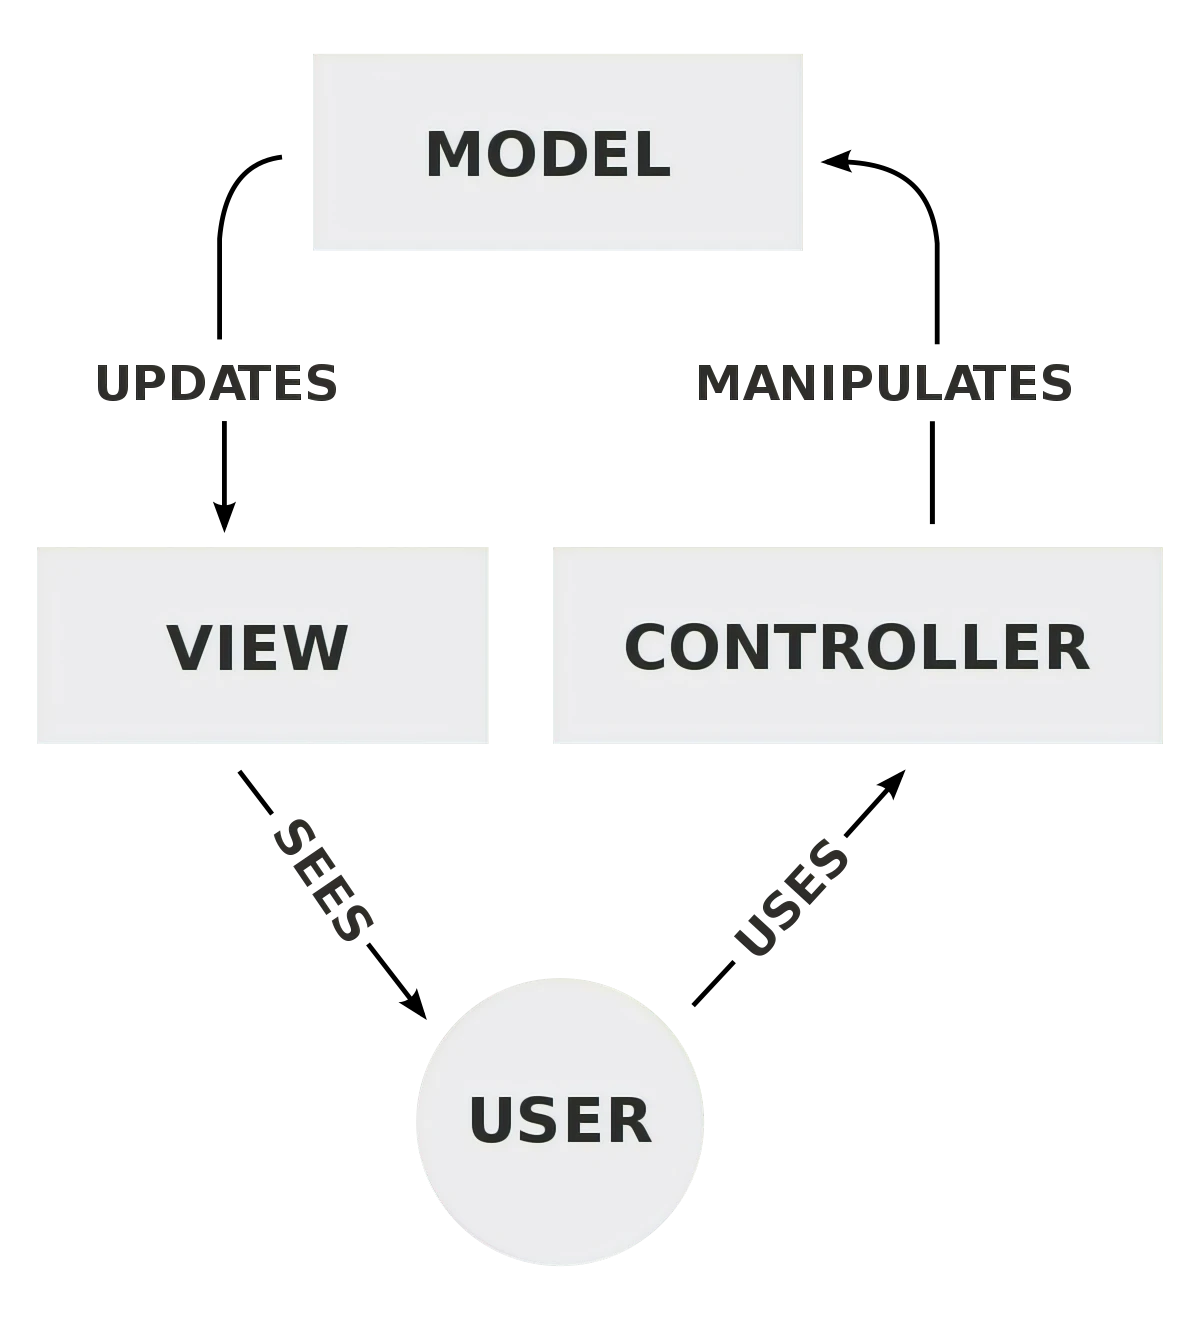
\includegraphics[width=2.5in]{./image/MVC.png}
  \end{center}
  \caption[MVC]{แผนผัง MVC หรือ Model-View-Controller~\cite{mvc}}
  \label{fig:MVC}
\end{figure}

\subsection{REST API}
REST API หรือ Representational State Transfer เป็นรูปแบบหนึ่งของ API (Application Programming Interface) ที่ทำการส่ง request และ response ผ่าน HTTP methods เช่น \textit{\texttt{Get}, \texttt{POST}, \texttt{PUT}, \texttt{DELETE}} เป็นต้น ผ่าน URL ของ API ที่ถูกออกแบบจัดสรรให้ทำหน้าที่ที่เฉพาะเจาะจงไว้เรียบร้อยแล้ว โดยเรียกได้อีกชื่อหนึ่งว่า \textbf{API Endpoints}

ซึ่งอุปกรณ์ของ client จำเป็นต้องส่ง request ไปยัง server ตาม endpoint ที่ถูกกำหนดหน้าที่การทำงานไว้แล้ว จากนั้น server จึงจะส่ง response กลับมาในรูปแบบใด ๆ ก็ได้ ซึ่งรูปแบบที่เป็นที่นิยมคือรูปแบบของ JSON

\begin{itemize}
  \item ข้อดีของ REST API มีดังนี้~\cite{rest_vs_soap}
  \begin{itemize}
    \item ทำงานอยู่บนมาตรฐานของ HTTP method
    \item รูปแบบของ response มีหลายรูปแบบเช่น JSON, XML เป็นต้น
    \item รองรับการขยายระบบได้ง่าย/มีความ independent สูง เพียงแค่ client เชื่อมต่อกับ endpoint ก็พอ
    \item รองรับการทำ caching โดยอาศัยหลักการของ API gateway
    \item เข้ากันกับรูปแบบการพัฒนาแบบ MVC เป็นอย่างดี
  \end{itemize}
  \item ข้อเสียของ REST API มีดังนี้
  \begin{itemize}
    \item ไม่มีการสนับสนุนเรื่อง security มาตั้งแต่ต้น เราจำเป็นต้อง implement เอง
    \item การทำ limitation ต่าง ๆ ของ request size, response size จำเป็นที่จะต้องออกแบบเองตั้งแต่ต้น
  \end{itemize}
\end{itemize}

\subsection{Cloud Based Development}
Cloud Based Development~\cite{cloud_dev} คือการพัฒนาโปรแกรมโดยอาศัย service ต่าง ๆ จากผู้ให้บริการ cloud (Cloud Provider) เพื่อลดค่าใช้จ่ายต่าง ๆ ที่จะเกิดจากการ host โปรแกรมของตนเอง เพราะการ host โปรแกรมหรือบริการของต้นเองนั้นใช้ต้นทุนสูงในการซื้อ hardware อีกทั้งยังตามมาด้วยค่าใช้จ่ายในการซ่อมบำรุงหรือขยาย service ของตนเอง ในปัจจุบัน Cloud Based Development จึงเป็นที่นิยมเพราะไม่ต้องจัดการปัญหาเหล่านั้นด้วยตนเองและง่ายต่อการ deploy อีกด้วย

ตัวอย่าง Cloud Provider ในปัจจุบัน เช่น Amazon Web Service (AWS), Google Cloud Platform (GCP), Google Firebase, Microsoft Azure เป็นต้น

\subsection{Component-driven Development}
Component-driven Development (CDD)~\cite{cdd} คือรูปแบบการพัฒนาโปรแกรมที่มีลักษณะพิเศษและสอดรับกับการพัฒนาด้วย React.js (ซึ่งเป็นเครื่องมือที่เราใช้ในโครงงานนี้) เป็นอย่างดี ด้วยการมองภาพส่วนของโปรแกรมต่าง ๆ เป็น component เพื่อความสะดวกและรวดเร็วในการพัฒนาและความเป็นระเบียบตาม design pattern แบบ command pattern
\begin{itemize}
  \item ประโยชน์ของ Component-driven Development
  \begin{itemize}
    \item ทำให้การทำงานกับนักออกแบบง่ายขึ้น เนื่องจากนักออกแบบจะเริ่มการออกแบบจาก design system ก่อน ซึ่งมีรูปแบบเป็น component-driven อยู่แล้ว
    \item สามารถแบ่งความรับผิดชอบภายในทีมได้ง่าย เช่น คนหนึ่งรับผิดชอบ component หนึ่งไปเลย เป็นต้น
    \item สามารถนำ component ต่าง ๆ กลับมาใช้ซ้ำ (reuse) ได้
  \end{itemize}
\end{itemize}

\section{User Interface}
\subsection{Progressive Web Application (PWA)}
Progressive web application (PWA)~\cite{pwa} คือการทําเว็บไซต์ธรรมดา ให้ใกล้เคียงกับแอปพลิเคชั่นที่ดาวน์โหลดลงเครื่องมากที่สุด ทั้งในแง่รูปลักษณ์ ความเร็ว ไปจนถึงการใช้งาน รวมถึงมีการปรับการแสดงผล
ให้เหมาะกับอุปกรณ์ที่ใช้ เช่น smartphone, tablet และ desktop

ลักษณะที่สําคัญที่สุดของ progressive web application แบ่งออกได้เป็นดังนี้ \\
\textbf{Reliable:} มีความน่าเชื่อถือ สามารถใช้งานได้ตลอดแม้ว่าการทํางานของเครือข่ายจะไม่เสถียร \\
\textbf{Fast:} ต้องเร็ว ไม่ว่าจะมีอนิเมชั่นสวยหรือสิ่งใดก็แล้วแต่ การตอบสนองต่อผู้ใช้สําคัญที่สุด \\
\textbf{Engaging:} ผู้ใช้สามารถใช้งานมันไม่ต่างกับแอปพลิเคชั่นปกติ

\begin{itemize}
  \item ข้อดีของ progressive web application มีดังนี้
  \begin{itemize}
    \item ลด learning curve ในการเรียนรู้เครื่องมือใหม่เพื่อที่จะพัฒนา mobile native application ทำให้ประหยัดเวลาในการพัฒนาและสามารถเอาเวลาที่ลดได้ไปโฟกัสในเรื่องอื่น ๆ เช่น การพิสูจน์ความต้องการของลูกค้าหรือตลาด เป็นต้น
  \end{itemize}
  \item ข้อเสียของ progressive web applications มีดังนี้~\cite{bad_pwa}
  \begin{itemize}
    \item การเข้าถึงในส่วนของ hardware เช่น กล้องถ่ายภาพ, geolocation, NFC, Bluetooth เป็นไปได้ยากและไม่มีการจดจำการอนุญาตเข้าถึง ทำให้ผู้ใช้งานจำเป็นที่จะต้องกดยินยอมในบางครั้ง
  \end{itemize}

\end{itemize}

\subsection{Responsive Web Design}
Responsive web design~\cite{responsive} เป็นเทคนิคการออกแบบเว็บไซต์ซึ่งจะมีการคํานึงถึงการปรับเปลี่ยนขนาดของเว็บไซต์ให้เหมาะสมกับการแสดงผลบนหน้าจอขนาดต่าง ๆ และความละเอียดของหน้าจอในอุปกรณ์ที่
แตกต่างกัน เช่น คอมพิวเตอร์ โน้ตบุ๊ค โทรศัพท์มือถือ แท็บเล็ต เป็นต้น เพื่อให้ประสบการณ์การใช้งานของ user ดีมากยิ่งขึ้น
\begin{itemize}
  \item ข้อดีของ responsive web design แบ่งออกได้เป็นดังนี้
  \begin{itemize}
    \item ทําให้เว็บไซต์รองรับอุปกรณ์มือถือไปในตัว (mobile-friendly) ซึ่งปั จจุบันจํานวนผู้ใช้งานเว็บไซต์จากโทรศัพท์มือถือนั้นกําลังเพิ่มมากขึ้น
    \item ผู้ใช้สามารถใช้งานเว็บไซต์ได้ง่าย (user-friendly) ไม่ว่าจะเปิดเว็บไซต์ด้วยอุปกรณ์หรือขนาดหน้าจอใด ๆ ก็ตาม
    \item สนับสนุนการทํา search engine optimization (SEO) กับ Google ทั้งเวอร์ชั่น desktop และ mobile ในเว็บไซต์เดียว
  \end{itemize}
  \item ข้อเสียของ responsive web design แบ่งออกได้เป็นดังนี้~\cite{bad_responsive}
  \begin{itemize}
    \item การใช้เขียน code รูปแบบเดียวเพื่อรองรับหลายอุปกรณ์ อาจทําให้เกิดปัญหาตามมาได้ ตัวอย่างเช่น ในโทรศัพท์มือถือที่มีหน้าจอขนาดเล็ก การซ่อนเนื้อหาที่ไม่จําเป็น เช่น โฆษณา ในบางเว็บบราวเซอร์จะยังทําการโหลดข้อมูลเหล่านี้เข้ามาแสดงอยู่
    \item Image resizing ที่ไม่ได้ลดขนาดของตัวรูปภาพ แต่ใช้วิธีการย่อขนาดขณะแสดงผลเท่านั้น ซึ่งอาจทําให้โทรศัพท์มือถือต้องโหลดรูปเดียวกับที่แสดงบน desktop จึงทําให้เราเสียเวลาโดยไม่จําเป็น
  \end{itemize}
\end{itemize}

\section{Best Practices}
\subsection{Timezone Complexity}
เมื่อมีการกระทำกับ attribute ของ record ใด ๆ ที่มี data type ในรูปแบบ \textit{\texttt{TIMESTAMP}} ทาง RDBMS จะทำการเก็บข้อมูลใน attribute นั้นใน format date-time แบบ UTC โดย default ซึ่งเมื่อเราจะใช้งานใน timezone อื่น ๆ ที่ไม่ใช่ UTC (เช่น GMT+0700 เป็นต้น) จะมีปัญหาในการ query ในแต่ละครั้งที่จะได้ผลลัพธ์ไม่ตรงกับ timezone ที่ client ใช้งานอยู่

\subsubsection{Best Practice}
TIMESTAMP ที่เก็บในฐานข้อมูลจะยังเป็น UTC format เหมือนเดิม แต่ทุกครั้งที่ query จะทำการ convert เป็น GMT ใด ๆ ก็ตามที่ client ได้ทำการ request มาทุกครั้งก่อนจะส่ง response กลับไป กล่าวคือ จากการแปลงตั้งแต่ต้นทางก่อนที่จะบันทึกเข้ามาในฐานะข้อมูล เราทำการแปลงก่อนจะส่ง response กลับไป เพื่อที่จะได้ง่ายต่อการทำงานเมื่อใช้งานจากต่างประเทศ

\subsection{Image Collection as Pool}
เมื่อเราต้องทำงานกับรูปภาพที่จะทำการบันทึกเข้ามายังฐานข้อมูล ความจริงแล้วมีวิธีการทำงานกับรูปภาพหลากหลายมาก เช่น การแปลงเป็น Base64 URL, การเก็บเป็น BLOB เป็นต้น แต่วิธีที่เป็นที่นิยมสำหรับการพัฒนาแบบ Cloud Based Development เป็นดังวิธีการดังนี้

\subsubsection{Best Practice}
เราจะทำการอัพโหลดรูปภาพหรือไฟล์ที่ต้องการขึ้นไปยัง cloud provider ที่เราเป็นสมาชิกเอาไว้ จากนั้นนำ URL ที่ได้หลังจากการอัพโหลดแล้วมาบันทึกในตาราง relation table ที่มี unique ID ของแต่ละ entity เอาไว้ เพื่อง่ายและสะดวกต่อการเรียกใช้หรือ CRUD ต่อไป

\subsection{JSX Coding Style Guide}
เป็นธรรมดาที่ว่าการเขียนโปรแกรมของแต่ละคนนั้นมีสไตล์การเขียนโค้ดหรือ convention~\cite{convention} ที่ต่างกัน ซึ่งมันจะไม่เป็นปัญหาหากเราทำงานเพียงคนเดียว แต่ในความเป็นจริงนั้นเราต้องทำงานกับทีมที่เกี่ยวข้องเราจึงต้องมี \textit{กฏหรือธรรมเนียมปฏิบัติในการเขียนโค้ด} เพื่อให้การทำงานเป็นทีมนั้นสะดวกและเป็นแบบแผนเดียวกันมากขึ้น

\subsubsection{Best Practice}
เราใช้ระเบียบแบบแผนของ Airbnb (Airbnb JSX Style Guide)~\cite{airbnb_jsx} เป็นข้อตกลงร่วมกันระหว่างคนในทีม ในการกำหนดสไตล์การเขียนโค้ดสำหรับโครงงานนี้

\section{ความรู้ตามหลักสูตรซึ่งถูกนำมาใช้หรือบูรณาการในโครงงาน}
\subsection{Usability Heuristic Evaluation}
\textit{จากวิชา 269462 Intro to Human-Computer Interaction} \\
หลักการทั้ง 10 ข้อเพื่อเป็น guideline สำหรับการออกแบบ User Interface ให้มี usability ที่ดีและเป็นเกณฑ์ตรวจสอบ UI คร่าว ๆ ว่า UI มีปัญหา usability ด้านไหน (Effectiveness/Efficiency/Satisfaction) โดยกระบวนการประเมิณผลโดยใช้หลักการนี้เรียกว่า ``Usability Heuristic Evaluation''

\subsection{Relational Database}
\textit{จากวิชา 261342 Fundamental of Database Systems และ 261343 Database Systems Laboratory} \\
ความรู้เกี่ยวกับการออกแบบฐานข้อมูล การสร้างแผนผัง Unified Modeling Language (UML) และ ER diagram

\subsection{Object-Oriented Programming}
\textit{จากวิชา 261200 Object-Oriented Programming} \\
ความรู้เกี่ยวกับการเขียนโปรแกรมเชิงวัตถุ ซึ่งเป็นแนวคิดในการพัฒนาซอฟแวร์ที่เป็นที่นิยมในปัจจุบัน โดยเฉพาะอย่างยิ่งรูปแบบการพัฒนาแบบ MVC

\subsection{Scrum}
\textit{จากวิชา 261361 Software Engineering} \\
ความรู้เกี่ยวกับการทำงานแบบ Scrum ที่มีความคล่องตัวสูงและเน้นผู้ใช้งานเป็นศูนย์กลาง (user-centric) โดยอาศัยการพัฒนาเป็นรอบ (sprint) เพื่อนำผลิตภัณฑ์ในแต่ละ sprint ออกไปทดสอบกับผู้ใช้งานหรือลูกค้าเพื่อในมาปรับแก้ให้สอดรับตามความต้องการ (requirement) ของผู้ใช้งานให้ได้มากที่สุด

\section{ความรู้นอกหลักสูตรซึ่งถูกนำมาใช้หรือบูรณาการในโครงงาน}
\subsection{Design Thinking}
เป็นกระบวนการตั้งแต่ก่อนการสร้างผลิตภัณฑ์ใด ๆ ไปจนถึงการนำผลิตภัณฑ์ไปทดสอบกับกลุ่มลูกค้าหรือผู้ที่ประสบปัญหานั้น ๆ ที่เราจะต้องการแก้ปัญหาให้ โดยผ่าน 5 ขั้นตอนสำคัญได้แก่ Empathize (การทำความเข้าอกเข้าใจปัญหา), Define (กำหนดปัญหาที่ต้องการจะแก้ไข), Ideate (ระดมไอเดียวิธีการแก้ไขปัญหา), Prototype (ทำตัวต้นแบบเพื่อนำไปทดสอบ), Test (ทดสอบเพื่อดูว่าไอเดียที่คิดสามารถแก้ไขปัญหาได้จริง)

\subsection{Problem-Solution Fit}
เป็นกระบวนการคิดแบบธุรกิจ startup ที่ต่อยอดมาจากกระบวนการ design thinking โดยก่อนที่จะดำเนินธุรกิจใด ๆ เราจำเป็นที่จะต้องให้ผลิตภัณฑ์ของเราตอบโจทย์ความต้องการของลูกค้าได้อย่างแท้จริงก่อน จึงจะสามารถดำเนินแผนธุรกิจอื่น ๆ เช่น การเก็บค่าบริการ, การขยายธุรกิจ ฯลฯ ต่อไปได้

\subsection{Business Model Canvas}
ตาราง 9 ช่องสำหรับการใส่รายละเอียดสำคัญก่อนเริ่มทำธุรกิจเพื่อเห็นภาพทั้งหมดก่อนว่าลักษณะธุรกิจของเราเป็นอะไร, ทำอะไร, เพื่อใคร รวมถึงกิจกรรมหลักทางธุรกิจต่าง ๆ, ต้นทุน, ช่องทางรายได้ที่จะได้รับด้วยเช่นกัน

amt.of timeslot = \text{places amt.entire~DB} \times ~\text{desks amt.entire~DB} \times ~\text{usable window}

\chapter{\ifproject%
\ifenglish Project Structure and Methodology\else โครงสร้างและขั้นตอนการทำงาน\fi
\else%
\ifenglish Project Structure\else โครงสร้างของโครงงาน\fi
\fi
}

\section{โครงสร้างของระบบ}
\subsection{System Architecture}
\subsubsection{Development Tools}
แพลตฟอร์ม Flowy และ Flowider พัฒนาในรูปแบบของระบบ client-server โดยในฝั่ง client พัฒนาด้วย React TS ควบคู่กับ Sass ที่เขียนผ่าน styled-component ในการทำหน้าที่สำหรับ styling ซึ่งการ initiate project เราได้ใช้งาน vite ซึ่งเป็น package provider ที่ขึ้นชื่อเรื่องความเร็วในการใช้งาน

สำหรับ server พัฒนาด้วย Express.js และ Node.js โดยมี Stripe ที่เป็น Payment Gateway Library มาช่วยในการพัฒนาส่วนของการชำระค่าบริการบนแพลตฟอร์ม ซึ่ง Stripe นั้นรองรับการชำระเงินที่หลากหลายรูปแบบและครอบคลุมหลากหลายประเทศทั่วโลก เช่น บัตรเครดิต/เดบิต, PromptPayQR เป็นต้น

และสุดท้ายสำหรับ database ได้เลือกใช้  MySQL ที่เป็นฐานข้อมูลแบบ relational database ควบคู่กับ Sequelize.js ในการ optimize แต่ละ query ให้มีประสิทธิภาพยิ่งขึ้น

\subsubsection{Deployment Tools}
ในด้านของการ deployment ทีมผู้พัฒนาได้เลือกใช้ Netlify ในการ publish ตัวของ user interface สำหรับฝั่ง server เราได้ใช้บริการของ Railway ในการทำ deploy API server และใช้ Amazon RDS, Firebase Storage ในเก็บข้อมูลที่เป็น relational database และไฟล์รูปภาพที่ใช้งานบนแพลตฟอร์ม ตามลำดับ
\begin{figure}[!ht]
    \begin{center}
    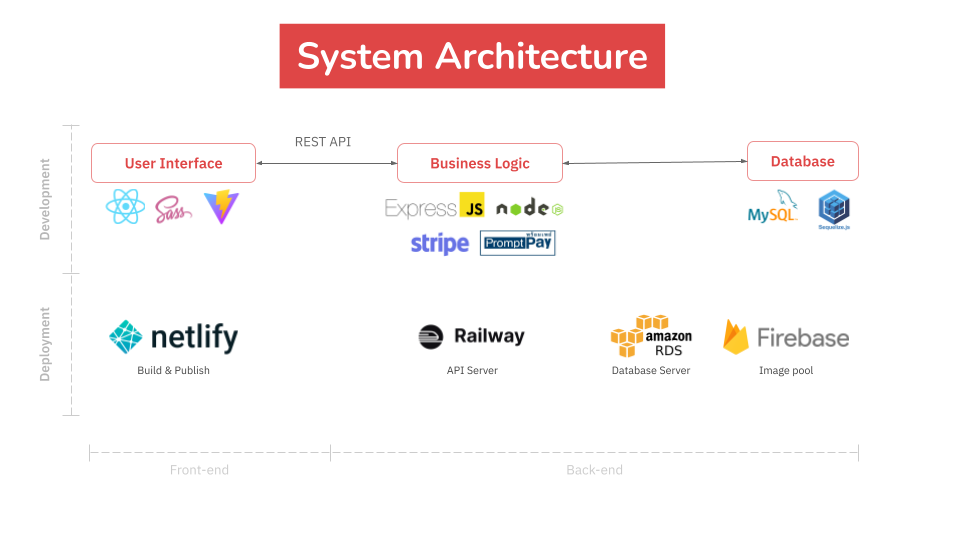
\includegraphics[width=\linewidth]{./image/System_Architecture.png}
    \end{center}
    \caption[System Architecture]{ภาพแสดงสถาปัตยกรรมระบบ}
    \label{fig:System_Architecture}
\end{figure}

\subsubsection{REST API}
แพลตฟอร์มของเราได้พัฒนาในรูปแบบของ MVC หรือ Model-View-Controller โดย Model คือ Database, Controller คือส่วนของ business logic หรือ server และสุดท้ายคือ View หรือ user interface อันเป็นส่วนที่ติดต่อกับผู้ใช้งาน

โดยการเชื่อมต่อระหว่างส่วนของ controller และส่วนของ view นั้น ได้เชื่อมต่อกันด้วย REST API กล่าวคือ หากจะต้องกระทำ business logic ใด ๆ หรือการ manipulate ใด ๆ กับ database ต้องกระทำด้วยการเรียกใช้งาน API endpoint ผ่าน HTTP methods เท่านั้น เช่น GET/POST/PUT/DELETE

ซึ่งประโยชน์ของการพัฒนาด้วย REST API คือการที่เราสามารถแยกส่วนของ user interface และ business logic ออกจากกันได้อย่างสิ้นเชิง โดยจุดนี้ได้อำนวยความสะดวกทีมผู้พัฒนาในการพัฒนาแต่ละส่วนโดยไม่จำเป็นต้องรอให้ส่วนใดส่วนหนึ่งพัฒนาเสร็จสิ้นก่อนจึงจะดำเนินการต่อได้ \\ \\
\begin{figure}[!ht]
    \begin{center}
    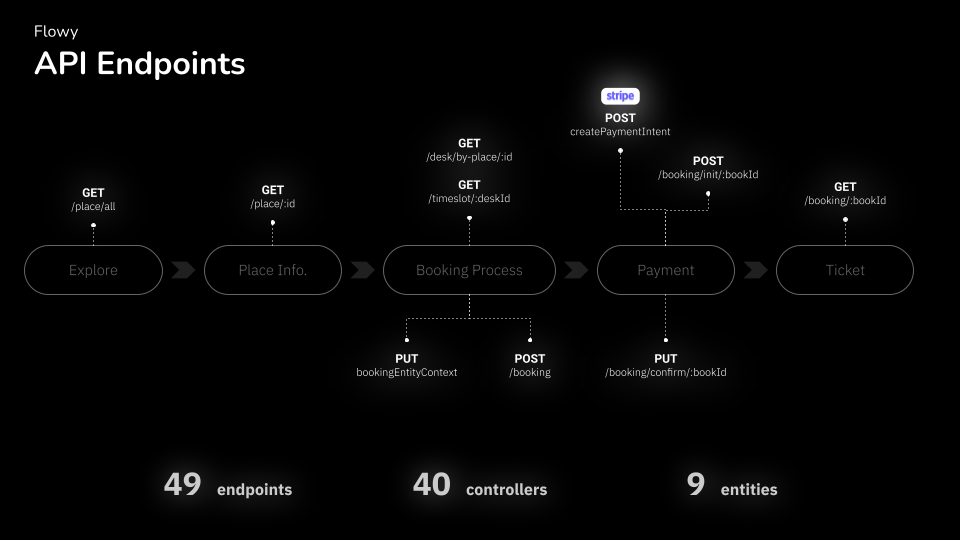
\includegraphics[width=\linewidth]{./image/API_Endpoints.png}
    \end{center}
    \caption[API Endpoints]{ภาพแสดงตัวอย่างของ API endpoint บางส่วนที่ได้ใช้งานบทแอปพลิเคชัน Flowy}
    \label{fig:API_Endpoints}
\end{figure}

\subsection{Database Design \& Schema}
ฐานข้อมูลที่เลือกใช้เป็นฐานข้อมูลประเภท SQL โดยมีองค์ประกอบดังรูปที่~\ref{fig:Database_schema_1} และมีรายละเอียดของข้อมูลดังต่อไปนี้ โดยเรียงลำดับตามแนวคิด parent entity ไปยัง children entity

\subsubsection{User}
เป็น entity ที่ใช้เก็บข้อมูลประจำตัวทั่วไปของผู้ใช้งานฝั่ง Flowy เพื่อใช้ระบุตัวตน (เมื่อทางราชการขอความร่วมมือ) และการเพื่ออำนวยความปลอดภัยให้กลับผู้ให้เช่าหรือ Flowider เมื่อเกิดเหตุการณ์ไม่พึงประสงค์ขึ้น ประกอบไปด้วย

\subsubsection{Flowider}
เป็น entity ที่ใช้เก็บข้อมูลประจำตัวทั่วไปของผู้ใช้งานฝั่ง Flowy เพื่อใช้ระบุตัวตน (เมื่อทางราชการขอความร่วมมือ), เพื่อทำการโอนเงินค่าใช้บริการจาก User และการเพื่ออำนวยความปลอดภัยให้กลับผู้เช่าหรือ Flowy เมื่อเกิดเหตุการณ์ไม่พึงประสงค์ขึ้น

\subsubsection{Place}
เป็น entity ที่ใช้เก็บข้อมูลรายละเอียดของสถานที่ที่ Flowider เป็นเจ้าของ เช่น ชื่อสถานที่, พิกัดของสถานที่, ที่อยู่เป็นลายลักษณ์อักษร, เวลาเปิด-ปิด เป็นต้น

\subsubsection{Amenity และ Specification}
เป็น 2 entities ที่ใช้เก็บรายละเอียดเพิ่มเติมของสถานที่นั้น ๆ ว่ามีลักษณะเป็นอย่างไร, เหมาะกับการใช้งานแบบไหนและมีสิ่งอำนวยความสะดวกใดให้บริการบ้าง เพื่อให้ user ใช้ประกอบการตัดสินใจได้ดียิ่งขึ้น

\subsubsection{Desk}
เป็น entity ที่ใช้เก็บข้อมูลจำเพาะของโซนโตะที่ให้บริการ โดยแนวคิดคือพื้นที่ของร้านต่าง ๆ จะถูกแบ่งออกเป็นโซนให้บริการ และเราจะเรียกแต่ละโซนเหล่านั้นว่า Desk ซึ่งแต่ละ Desk ใน entity นี้นั้นไม่จำเป็นต้องมีแค่โต๊ะเดียวตามชื่อของ entity ก็ได้

ซึ่ง attribute ในนี้จะเก็บค่าที่จำเป็นต่อการจองต่าง ๆ เช่น ที่นั่งต่ำสุดที่เข้าใช้งานได้รวมถึงจำนวนคนสูงสุดที่จะเข้าใช้งานได้, ประเภทของโต๊ะว่าเป็น Hot Desk รึเปล่า เป็นต้น (Hot Desk คือรูปแบบการจัดพื้นที่สำนักงานโต๊ะส่วนกลาง ที่เน้นตอบโจทย์เรื่องของ Open Space และความยืดหยุ่นในการทำงานและอิสระของพนักงานมากยิ่งขึ้นโดยให้พนักงานในองค์กรสามารถมาใช้โต๊ะทำงานส่วนกลางในเวลาใดก็ได้ ตำแหน่งไหนก็ได้)

\subsubsection{Timeslot}
เป็น entity ที่ใช้เก็บ time slot ทั้งหมดที่ถูก generate โดยอัตโนมัติจากเวลาที่ตั้งไว้บน server และค่าที่เปลี่ยนแปลงได้มีเพียงแค่ status และ occupied\_seat ที่บ่งบอกสถานะการใช้งานและจำนวนคนที่เข้าใช้งานตามลำดับ

\subsubsection{Booking}
เป็น entity ที่ใช้เก็บรายละเอียดสำคัญที่เกี่ยวข้องการจองทั้งหมดรวมถึงรายละเอียดและสถานะของการชำระค่าบริการด้วยเช่นกัน

\begin{landscape}
    \begin{figure}[ht]
        \begin{center}
            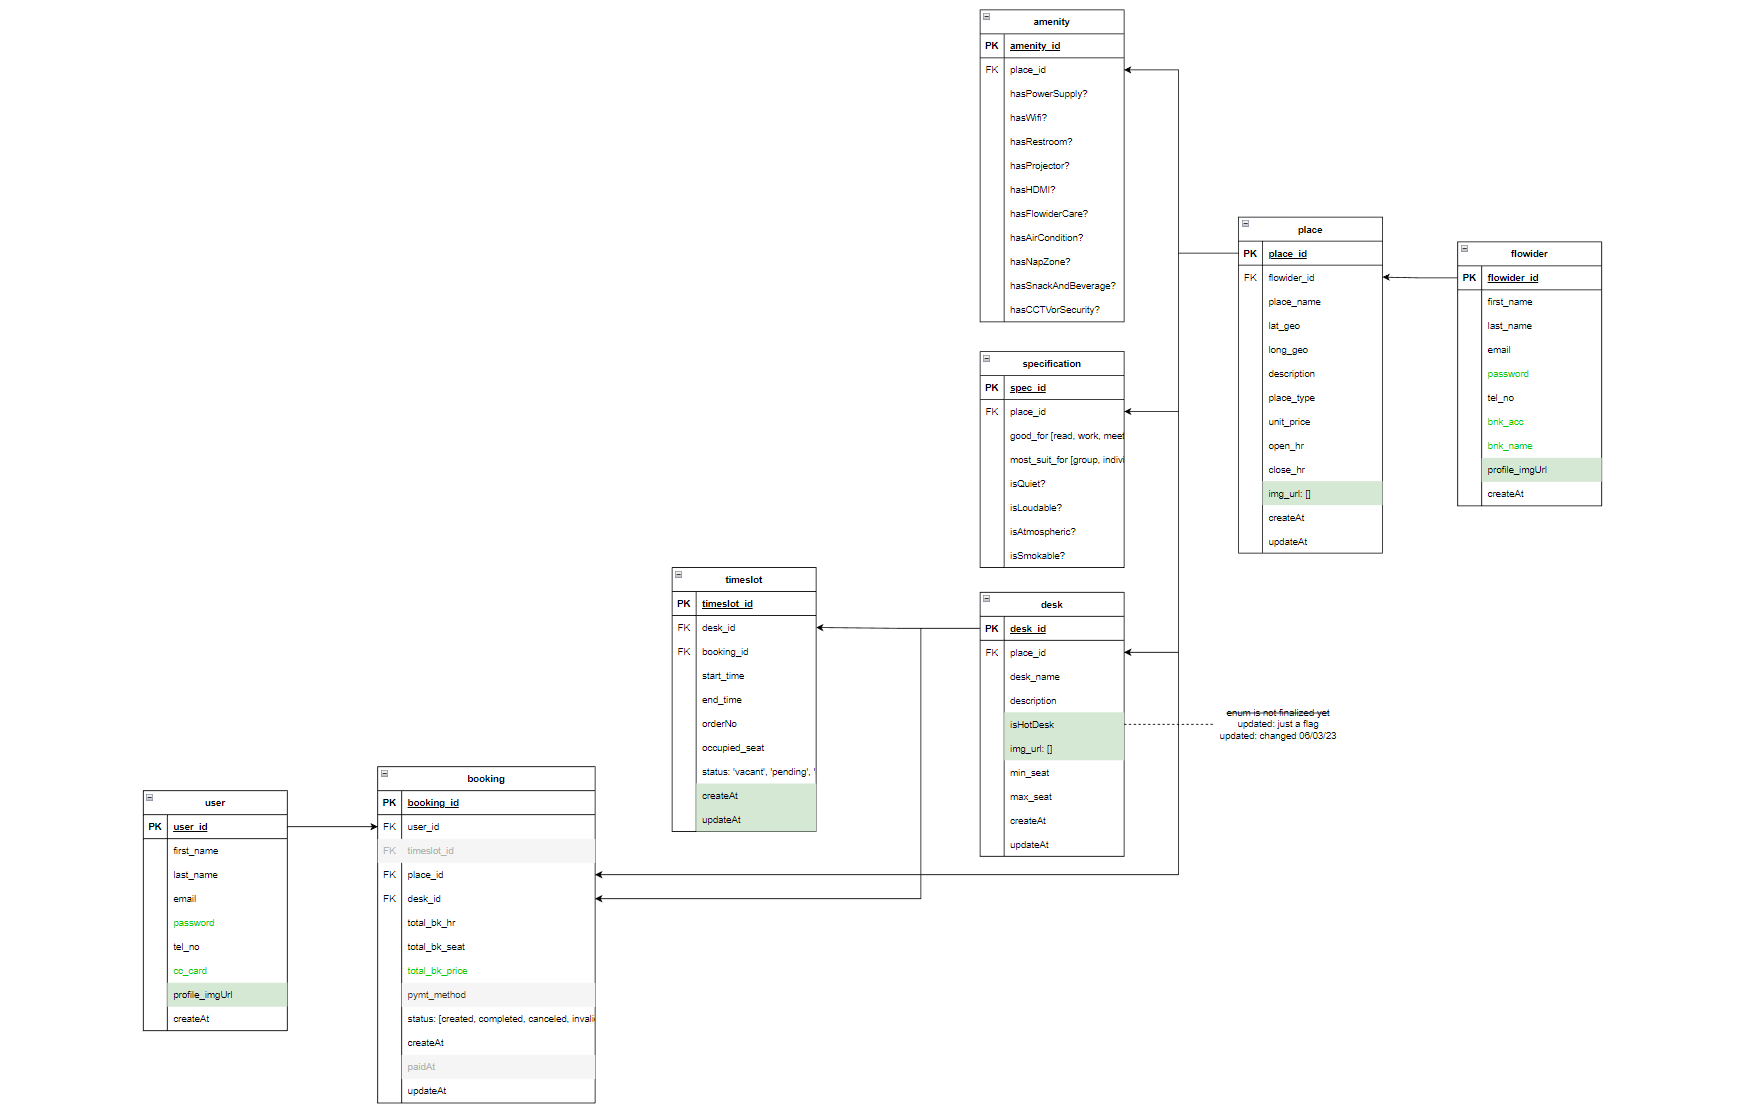
\includegraphics[width=8.1in]{./image/Database_schema_1.png}
        \end{center}
        \caption[Database Schema]{แผนภาพแสดงโครงสร้างของฐานข้อมูล}
        \label{fig:Database_schema_1}
    \end{figure}
\end{landscape}

\subsection{Time Slot Design}
\subsubsection{Generation Logic}
การออกแบบการทำงานของการเลือกช่วงเวลาใช้บริการที่แยกตามแต่ละ Desk นั้นถือเป็นหนึ่งในความท้าทายของโครงงานนี้ เนื่องจากมีแนวคิดหลากหลายรูปแบบที่เราสามารถนำมาปรับใช้ได้ โดยเบื้องต้นเราได้นึกถึงการจองตั๋วเพื่อเข้าชมภาพยนตร์ แต่แนวคิดนี้ก็ตกไปเนื่องจากติดปัญหาในส่วนของผังที่นั่งที่จัดวางไม่เหมือนกันในแต่ละร้าน ซึ่งแตกต่างกับโรงภาพยนตร์ที่มีผังที่นั่งชัดเจนอย่างสิ้นเชิง

ในแนวความคิดต่อมาคือเพิ่มความ abstract มากขึ้นด้วยการเปลี่ยนเป็นแสดงผลแค่ช่วงเวลาอย่างเดียว แล้วให้ผู้ใช้งานกดเลือกช่วงเวลาที่ต้องการใช้งานเท่านั้น แต่เริ่มต้นเราต้องการให้ฝั่งของ user interface เป็นฝ่าย generate time slot ทั้งหมดตามเงื่อนไขเวลาเปิด-ปิดทำการของสถานที่นั้น เมื่อผู้ใช้งานเลือกก็ส่งรายละเอียดต่าง ๆ เข้ามายัง entity Timeslot ก็เป็นอันเสร็จสิ้น แต่แนวคิดนี้ก็ตกไปเช่นกันเนื่องจากการทำงานที่หนักเกินไปของฝั่ง user interface และติดปัญหาเรื่อง reference เวลาทำ payment process

สุดท้ายเราจึงเลือกวิธีการ generate time slot ทั้งหมดโดยอัตโนมัติผ่านการทำงานของ business logic โดยมีหลักการคิดคือคำนวณหาผลต่างของเวลาเปิด-ปิด (usable window) ของแต่ละสถานที่ แล้วนำไปสร้าง time slot ใหม่ให้แต่ละโต๊ะ ในทุก ๆ โต๊ะ, ทุก ๆ ร้าน และทุก ๆ วัน

\begin{equation}
    amt.\;of\;timeslot = places\;amt.\;entire\;DB\times desks\;amt.\;entire\;DB \times usable\;window
\end{equation}

ตัวอย่างเช่น หากแพลตฟอร์มของเรามีทั้งหมด 10 สถานที่ แต่ละที่มี usable window จากการคำนวณเวลาเปิด-ปิด 10 ชั่วโมงเหมือนกันทุกร้าน และแต่ละสถานที่มีทั้งหมด 10 โต๊ะเหมือนกันหมด ก็จะคำนวณได้ว่า

\begin{equation}
    amt.\;of\;timeslot = 10 \times 10 \times 10
\end{equation}

ในวันต่อ ๆ ไปหากไม่มีจำนวนร้านหรือโต๊ะเพิ่มขึ้นเลย แต่ละวันจะมี time slot ถูก generate ขึ้นวันละ 1000 time slots ซึ่งเราได้ทำการเขียนคำสั่งที่คอยลบ time slot ที่มีสถานะ *vacant* ไว้แล้วในทุก ๆ สัปดาห์ เพื่อลดปัญหาการใช้พื้นที่ฐานข้อมูลเกินจำเป็น

ซึ่งจากวิธีการนี้ทำให้เราลดภาระการทำงานของ user interface ได้ รวมถึงลดความยุ่งยากของทีมผู้พัฒนาด้วยเช่นกัน

\subsubsection{Component Design}
เมื่อเราได้วิธีการในการสร้าง time slot แล้ว ในส่วนต่อไปคือการออกแบบการทำงานของ user interface ที่จะทำให้การปรับเปลี่ยนรายละเอียดของ time slot มีประสิทธิภาพที่สุด เราจะได้ใช้หลักแนวคิดแบบ immutable component กล่าวคือเราจะไม่ทำการปรับเปลี่ยนค่าใด ๆ ของ time slot ทั้งสิ้น และยกหน้าที่การเปลี่ยนแปลงค่าต่าง ๆ ให้กับ business logic เท่านั้น

เพราะฉะนั้นสิ่งที่เราทำคือการสร้าง array ออกมา 1 arrays คือ chosenTimeSlot ที่เป็น array ของ time slot ที่ถูกกดเลือกเอาไว้ เพื่อเก็บ object ของ time slot เอาไว้ เตรียมส่งกลับไปให้ business logic ดำเนินการต่อ

เมื่อผู้ใช้งานทำการกดเลือก เราจะทำการ push object ของ time slot นั้น เข้าสู่ chosenTimeSlot และทำการ pop ออกจาก chosenTimeSlot เมื่อมีการกดอีกครั้งหนึ่ง (เป็นการยกเลิกการเลือก) ในขณะเดียวกันกับที่เกิด action เหล่านี้ ก็ต้องทำการเปลี่ยน styling ที่แสดงผล time slot ที่ถูกเลือกด้วยการใช้งาน state ของ React TS ด้วยเช่นกัน เมื่อสิ้นสุดการเลือกแล้ว ค่าใน chosenTimeSlot คือสิ่งที่เราจะใช้ต่อไปในส่วนของ business logic

\subsection{Payment Process}
ระบบชำระค่าบริการเป็นส่วนที่ท้าทายที่สุดในโครงงานนี้ เนื่องจากเป็นส่วนที่ละเอียดอ่อนและต้องทำงานกับ credential ของผู้ใช้งาน หากเกิดปัญหาจากการใช้งานอาจทำให้เกิดการฟ้องร้องเอาผิดขึ้นมาได้ ทางทีมผู้พัฒนาจึงใช้บริการของ Stripe ซึ่งเป็น payment gateway provider ที่ผู้ประกอบการหรือนักพัฒนาซอฟต์แวร์ทั่วโลกเลือกใช้งาน ตัวอย่างประโยชน์ของการใช้งาน Stripe เช่น
\begin{itemize}
    \item มีตัวเลือกการชำระเงินครอบครัวเกือบทุกรูปแบบในทุกประเทศทั่วโลก
    \item มี documentation ที่ดี ปฏิบัติตามได้อย่างไม่สับสน
    \item มี developer community ที่กว้างขวาง พร้อมช่วยเหลือเมื่อเกิดปัญหา เนื่องจาก Stripe ถูกใช้งานกว่า 1,000,000 เว็บไซต์ทั่วโลก
    \item implementation ง่าย ขั้นตอนไม่ยุ่งยาก
\end{itemize}
เนื่องจากทีมผู้พัฒนาไม่มีประสบการณ์การทำระบบชำระค่าบริการมาก่อน จึงต้องการทำความเข้าใจโดยละเอียดทั้งหมดถึงกระบวนการจองไปจนถึงการชำระค่าบริการ ว่าเราจะต้องทำการส่งผ่าน/เปลี่ยนค่าของรายละเอียดการจองอย่างไร และจะติดต่อกับ Stripe API, Flowy API ได้อย่างไร

เราจึงทำการวาด service blueprint ดังรูปที่~\ref{fig:service_blueprint} เพื่อทำให้ทีมผู้พัฒนาเห็นภาพร่วมกันว่า ลักษณะโครงสร้างการทำงานจะมีลักษณะเช่นไร และทำให้ผู้พัฒนาสามารถปรับปรุงการส่งผ่านรายละเอียดการจองเป็นไปได้อย่างมีประสิทธิภาพมากยิ่งขึ้น

\subsection{UX/UI Design}
\subsubsection{Flowy}
\begin{itemize}
    \item Login: หน้าเข้าสู่ระบบสําหรับผู้ใช้งาน (รูปที่~\ref{fig:Flowy_login})
    \item Register: หน้าสมัครสมาชิกสําหรับผู้ใช้งาน (รูปที่~\ref{fig:Flowy_register})
    \item Explore: หน้าแสดงสเปซที่ให้บริการบนแพลตฟอร์ม Flowy (รูปที่~\ref{fig:Flowy_explore})
    \item Place information: หน้าแสดงรายระเอียดของสเปซ (รูปที่~\ref{fig:Flowy_info_1} และ~\ref{fig:Flowy_info_2})
    \item Booking
    \begin{itemize}
        \item Booking customer amount: หน้าระบุจํานวนผู้เข้าใช้บริการ (รูปที่~\ref{fig:Flowy_book_ctm_amt})
        \item Booking desk: หน้าเลือกโต๊ะสําหรับทํากิจกรรมต่าง ๆ (รูปที่~\ref{fig:Flowy_book_desk})
        \item Booking time slot: หน้าระบุเวลาเข้าใช้บริการ (รูปที่~\ref{fig:Flowy_book_time_slot})
    \end{itemize}
    \item Payment: หน้าชําระค่าบริการ (รูปที่~\ref{fig:Flowy_payment})
    \item Ticket: หน้าแสดงรายระเอียดตั๋ว (รูปที่~\ref{fig:Flowy_ticket_1} และ~\ref{fig:Flowy_ticket_2})
    \item Account: หน้าแสดงบัญชีผู้ใช้ (รูปที่~\ref{fig:Flowy_account})
    \item Booking history: หน้าแสดงประวิติการจองสเปซ (รูปที่~\ref{fig:Flowy_book_history})
\end{itemize}

\subsubsection{Flowider}
\begin{itemize}
    \item Login: หน้าเข้าสู่ระบบสําหรับผู้ใช้งาน (รูปที่~\ref{fig:Flowider_login})
    \item Register: หน้าสมัครสมาชิกสําหรับผู้ใช้งาน (รูปที่~\ref{fig:Flowider_register})
    \item Booking management: หน้าจัดการรายการจอง (รูปที่~\ref{fig:Flowider_booking_mgmt})
    \item Schedule: หน้าแสดงรายระเอียดการจองของแต่ละสเปซ (รูปที่~\ref{fig:Flowider_schedule})
    \item Account: หน้าแสดงบัญชีผู้ใช้ของผู้ใช้บริการ (รูปที่~\ref{fig:Flowider_account})
    \item Edit account: หน้าแก้ไขข้อมูลส่วนตัวของผู้ให้บริการ (รูปที่~\ref{fig:Flowider_edit_account})
    \item Space management: หน้าจัดการสเปซ (รูปที่~\ref{fig:Flowider_space_mgmt})
    \item Edit Space: หน้าแก้ไขข้อมูลของสเปซ (รูปที่~\ref{fig:Flowider_space_edit_1} และ~\ref{fig:Flowider_space_edit_2})
    \item Create place
    \begin{itemize}
        \item Onboarding: หน้าเตรียมข้อมูลของสเปซก่อนทําการลงทะเบียน (รูปที่~\ref{fig:Flowider_onboarding_1}) และหน้าเตรียมข้อมูลของโต๊ะก่อนทําการลงทะเบียน (รูปที่~\ref{fig:Flowider_onboarding_2})
        \item Place category: หน้าระบุประเภทของสเปซ (รูปที่~\ref{fig:Flowider_place_category})
        \item Place information: หน้าระบุรายละเอียดของสเปซ (รูปที่~\ref{fig:Flowider_place_info_1} และ~\ref{fig:Flowider_place_info_2})
        \item Specification: หน้าระบุความเฉาะเจาะจง (รูปที่~\ref{fig:Flowider_place_Specification})
        \item Amenity: หน้าระบุสิ่งอํานวยความสะดวก (รูปที่~\ref{fig:Flowider_place_amenity})
        \item Place image upload: หน้าเพิ่มรูปภาพของสเปซ (รูปที่~\ref{fig:Flowider_place_img})
        \item Place location: หน้าระบุตําแหน่งของสเปซ (รูปที่~\ref{fig:Flowider_place_location})
        \item Desk: หน้าระบุรายระเอียดของโต๊ะ (รูปที่~\ref{fig:Flowider_desk_1} และ~\ref{fig:Flowider_desk_2})
    \end{itemize}
\end{itemize}

\section{ขั้นตอนการดำเนินงาน}
\subsection{ทำความเข้าใจปัญหา}
เนื่องจากพวกเราเป็นนักศึกษามหาวิทยาลัย ทุกช่วงที่การสอบกลางภาคหรือปลายภาคใกล้เข้ามา เรามันจะปัญหาในเรื่องของการไม่มีพื้นที่ที่เพียงพอสำหรับทำกิจกรรมต่าง ๆ เช่น การอ่านหนังสือ, ทำงานกลุ่มหรือประชุม เป็นต้น ทำให้เราเริ่มมีความคิดว่า ``ปัญหานี้มักจะเกิดมาจากปริมาณการใช้งานในเวลาที่ใกล้เคียงกันโดยอุปทานหรือพื้นที่ที่ให้ใช้สอยมีไม่เพียงพอต่อความต้องการ''

เมื่อเราพบเจอกับปัญหาเช่นนี้แล้ว เราจึงคิดต่อไปว่าอยากที่จะแก้ไขปัญหานี้ แต่ก่อนที่จะเริ่มขั้นตอนการพัฒนาผลิตภัณฑ์หรือ solution ใดที่จะเข้ามาแก้ปัญหา เราต้องการแน่ใจก่อนว่าปัญหาที่เราเจอไม่ได้มีเพียงเราเจอแค่กลุ่มเดียวหรือแค่กลุ่มเล็ก ๆ เท่านั้น เราจึงทำการออกแบบสำรวจเพื่อทำการสำรวจปัญหาและทำความเข้าใจปัญหาเพิ่มเติมในเชิงลึกขึ้นถึงความต้องการที่แท้จริงของผู้ประสบปัญหาที่คล้ายคลึงกับเรา

โดยทั้งหมดที่กล่าวมานี้ คือขั้นตอนแรกของกระบวนการ Design Thinking นั่นคือ ``การทำความเข้าอกเข้าใจ (Empathize)''

\subsection{กำหนดปัญหาและทำแบบสำรวจ}
ในการทำแบบสำรวจได้ถูกแบ่งออกเป็น 3 ส่วนด้วยกัน ดังนี้
\begin{enumerate}
    \item คำถามทั่วไป (General Question)
    \begin{itemize}
        \item เพศ
        \item อายุ
        \item อาชีพ
        \item รับดับการศึกษาสูงสุด
        \item ชื่อสถานศึกษา
        \item คณะที่กำลังศึกษา
        \item รายได้เฉลี่ยในแต่ละเดือน
    \end{itemize}
    \item คำถามเชิงพฤติกรรม (Behavioral Question)
    \begin{itemize}
        \item โดยลักษณะนิสัยของท่านแล้ว ท่านชอบอ่านหนังสือ / ทำงานคนเดียวหรือเป็นกลุ่ม
        \item โดยปกติแล้วคุณอ่านหนังสือเพื่อเตรียมตัวสอบที่ใด
        \item โดยปกติแล้วคุณทำงานกลุ่ม / ทำงานบริษัทที่ใด
        \item ความสะดวกจากการใช้งานสถานที่เหล่านั้น
        \item ท่านมักเจอปัญหาอะไรจากสถานที่ที่คุณใช้บริการอ่านหนังสือ / ทำงานบ้าง
        \item โดยปกติแล้วท่านแก้ไขปัญหาเหล่านั้นอย่างไร
    \end{itemize}
    \item คำถามเพื่อหาวิธีการแก้ไขปัญหา (Solution Finding)
    \begin{itemize}
        \item หากมีตัวช่วยที่สามารถแก้ไขปัญหาการหาที่อ่านหนังสือ / ทำงานดังที่ท่านได้ระบุก่อนหน้านี้ได้ ท่านมีความสนใจมาก-น้อยเท่าใด
        \item ตัวช่วยดังกล่าวจะมีลักษณะคล้ายคลึงกับ Airbnb สำหรับการหาที่อ่านหนังสือ / ทำงาน (คือมีลักษณะเป็นการเช่าพื้นที่ของเจ้าของที่พักเป็นรายชั่วโมง แทนที่จะเป็นการเช่าที่พักรายคืนเหมือน Airbnb) ท่านมีความสนใจที่จะใช้งานมากเพียงใด
        \item ความเร่งด่วนที่ต้องการตัวช่วยนี้เข้ามาทำให้ชีวิตคุณสะดวกมากขึ้น มีมาก-น้อยเพียงใด
        \item คุณต้องการใช้งานตัวช่วยนี้ผ่านอุปกรณ์ประเภทใดมากที่สุด
        \item คุณต้องการให้สถานที่อ่านหนังสือ / ทำงานนั้นๆ ต้องมีสิ่งอำนวยความสะดวกอะไรบ้าง
        \item ราคาในใจสูงสุดที่จะยอมจ่ายเพื่อเช่าสถานที่นั้น จะมีราคาเท่าใดต่อ 1 ชั่วโมง
        \item ท่านมีแนวโน้มจะใช้ตัวช่วยนี้กับเพื่อนของคุณมากน้อยเพียงใด
        \item ท่านคาดหวังที่จะได้ประสบการณ์การใช้งาน (user experience) จากตัวช่วยนี้อย่างไรบ้าง
        \item คำแนะนำเพิ่มเติมถึงผู้พัฒนา
    \end{itemize}
\end{enumerate}

\subsection{ออกแบบ Proof of Concept}
เมื่อได้ผลสำรวจมาแล้ว เราจึงเริ่มออกแบบตัวต้นแบบของเราด้วยการวิเคราะห์ปัญหาและความต้องการของผู้ทำแบบสำรวจ เพื่อให้การใช้งานและประสบการณ์ใช้งานราบรื่นที่สุด
\begin{itemize}
    \item ออกแบบตัวต้นแบบ UX/UI ด้วย \href{https://www.figma.com/file/y0b4Wo3axU0TD5uoZHBhZM/Flowy?node-id=0-1&t=JYeTFmvNhNrmnj4b-0}{Figma}
    \item ออกแบบโครงสร้างแพลคฟอร์มและฐานข้อมูลด้วย \href{https://app.diagrams.net/#G1SVEf5xnuNXJhE77jdD0Rvaj5KxYkY-5y}{Draw.io}
\end{itemize}

\subsection{พัฒนาระบบ}
\begin{itemize}
    \item พัฒนาในส่วนของ user interface ตามที่ได้ทำการออกแบบ UX/UI
    \item พัฒนาในส่วนของ server ตามกระบวนการพื้นฐาน CRUD โดยใช้โปรแกรม Postman ในการทดสอบ API endpoint ต่าง ๆ
    \item พัฒนาโครงสร้างของ database ตาม schema ที่ได้ทำการออกแบบ โดยทดสอบหรือ query ตรวจสอบความถูกต้องของข้อมูลโดยไม่ผ่าน API endpoint ด้วย MySQL Workbench 8.0 CE ที่เชื่อมต่อโดยตรงกับ AWS RDS
\end{itemize}

\subsection{การทดสอบใช้งาน}
\begin{itemize}
    \item ทำการทดสอบระบบในแต่ละ function ในแต่ละหน้าทั้งแพลตฟอร์ม Flowy และ Flowider ว่าสามารถทำงานได้ถูกต้อง
    \item ทำการทดสอบการใช้งานในแต่ละ feature ของทั้งแพลตฟอร์ม Flowy และ Flowider ว่าการใช้งานราบรื่น ไม่มีส่วนใดผิดปกติ
    \item วางแผนการทดสอบการใช้งานแบบสาธารณะในเดือนมีนาคม 2566
\end{itemize}

% \begin{landscape}
%     \begin{figure}[ht]
%         \begin{center}
%             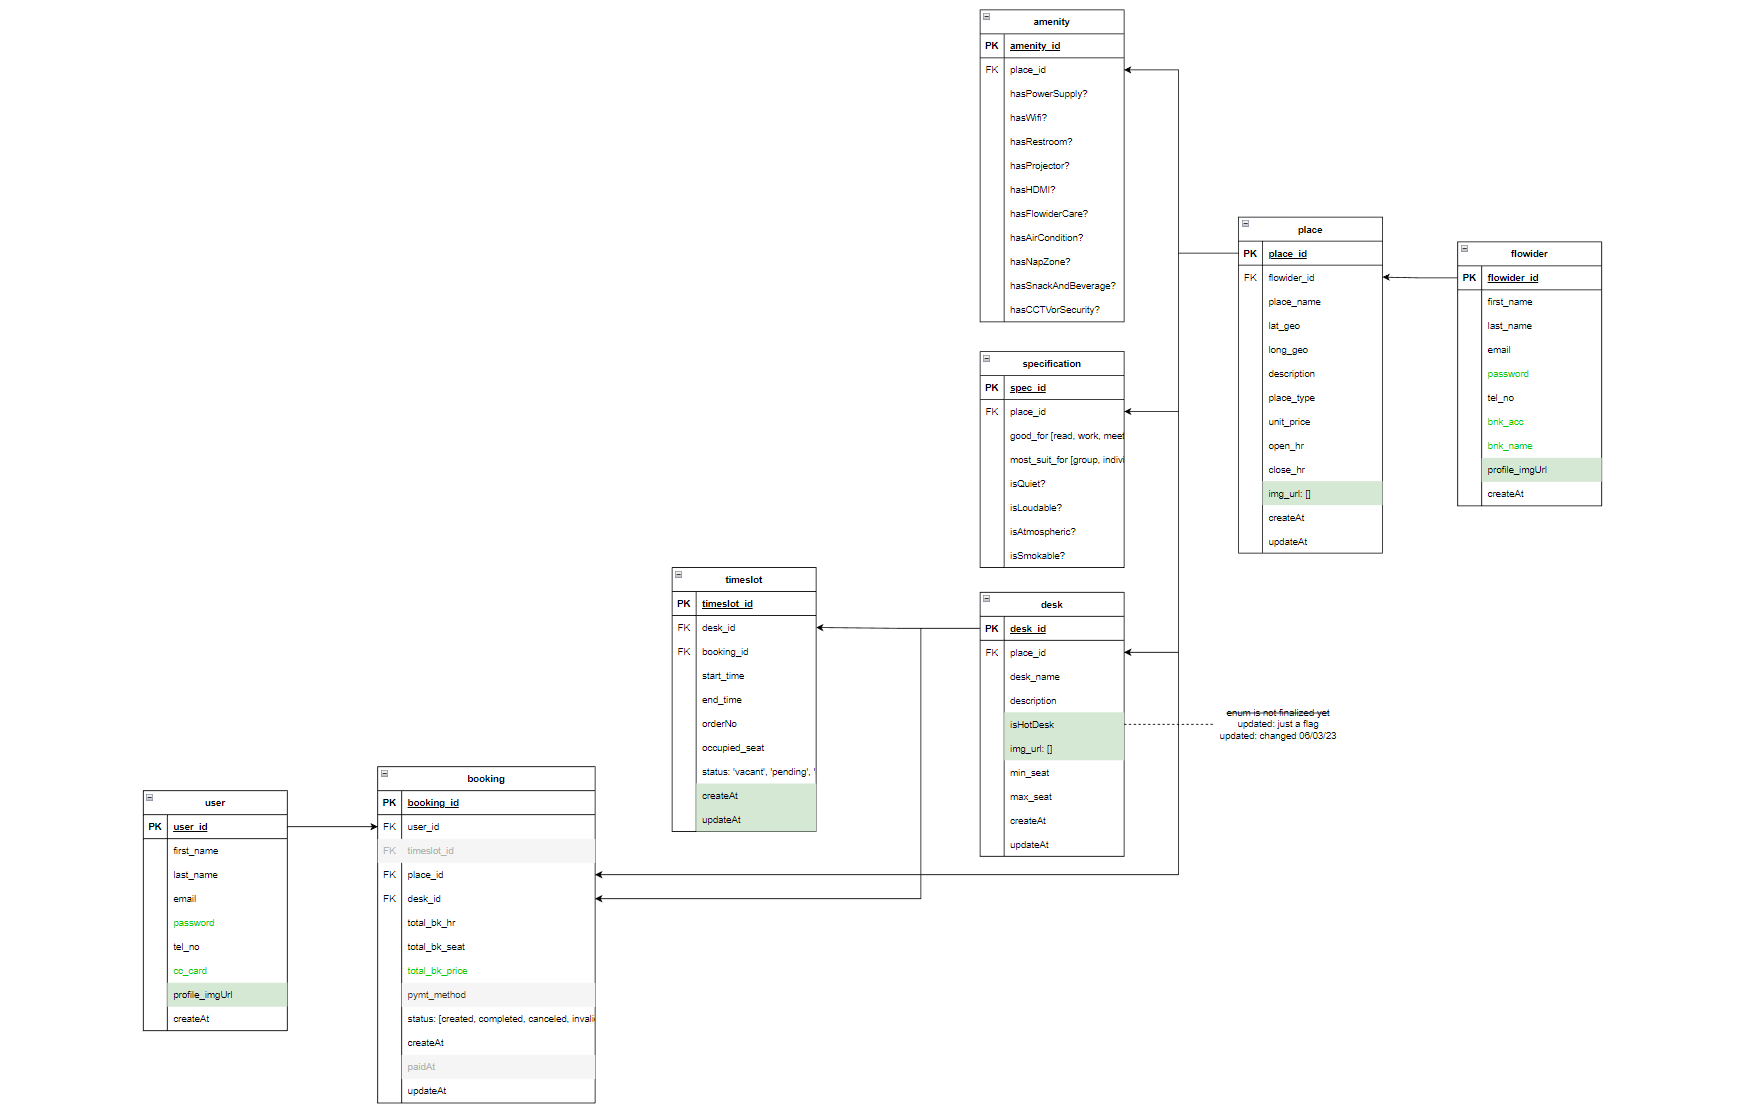
\includegraphics[width=8.1in]{./image/Database_schema_1.png}
%         \end{center}
%         \caption[Database Schema]{แผนภาพแสดงโครงสร้างของฐานข้อมูล}
%         \label{fig:Database_schema_1}
%     \end{figure}
% \end{landscape}
\begin{landscape}
    \begin{figure}[ht]
        \begin{center}
        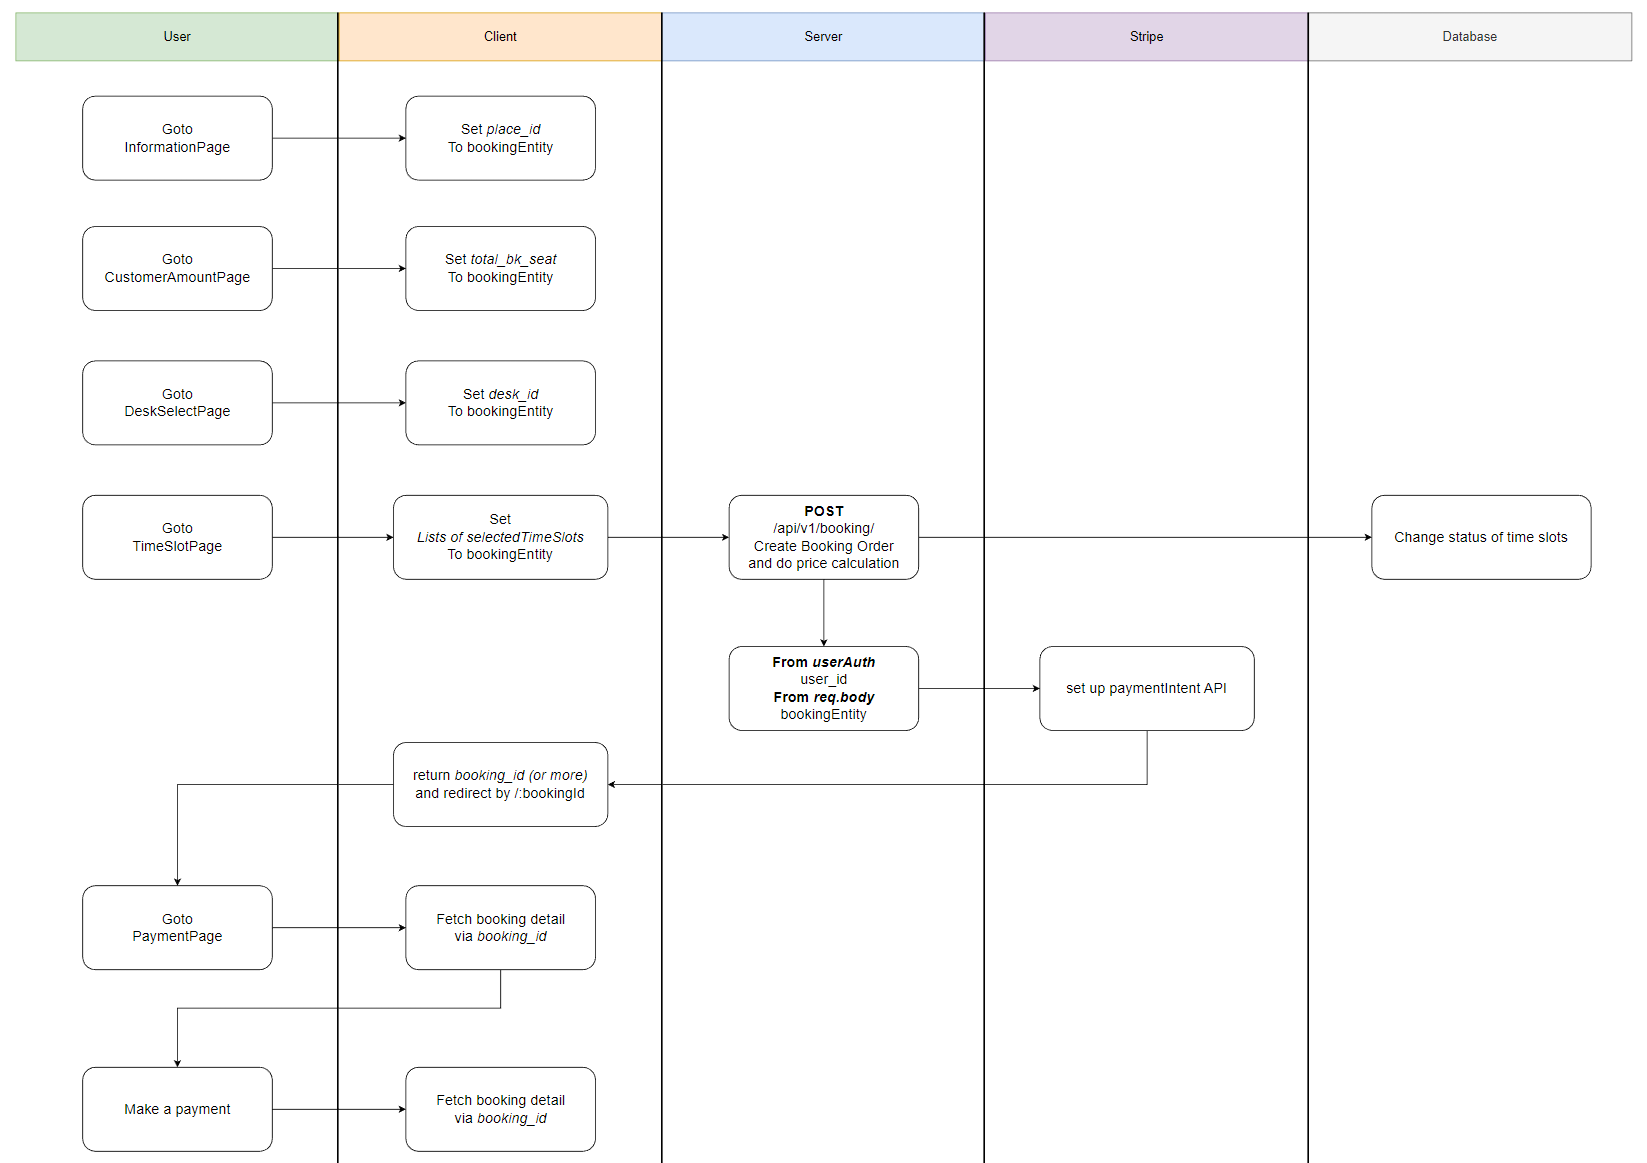
\includegraphics[width=7in]{./image/service_blueprint.png}
        \end{center}
        \caption[Payment service blueprint]{แผนผัง service blueprint การทำงานทั้งหมดของกระบวนการจองตั้งแต่เริ่มต้นจนถึงชำระค่าบริการ}
        \label{fig:service_blueprint}
    \end{figure}
\end{landscape}
\begin{figure}[t]
    \begin{center}
    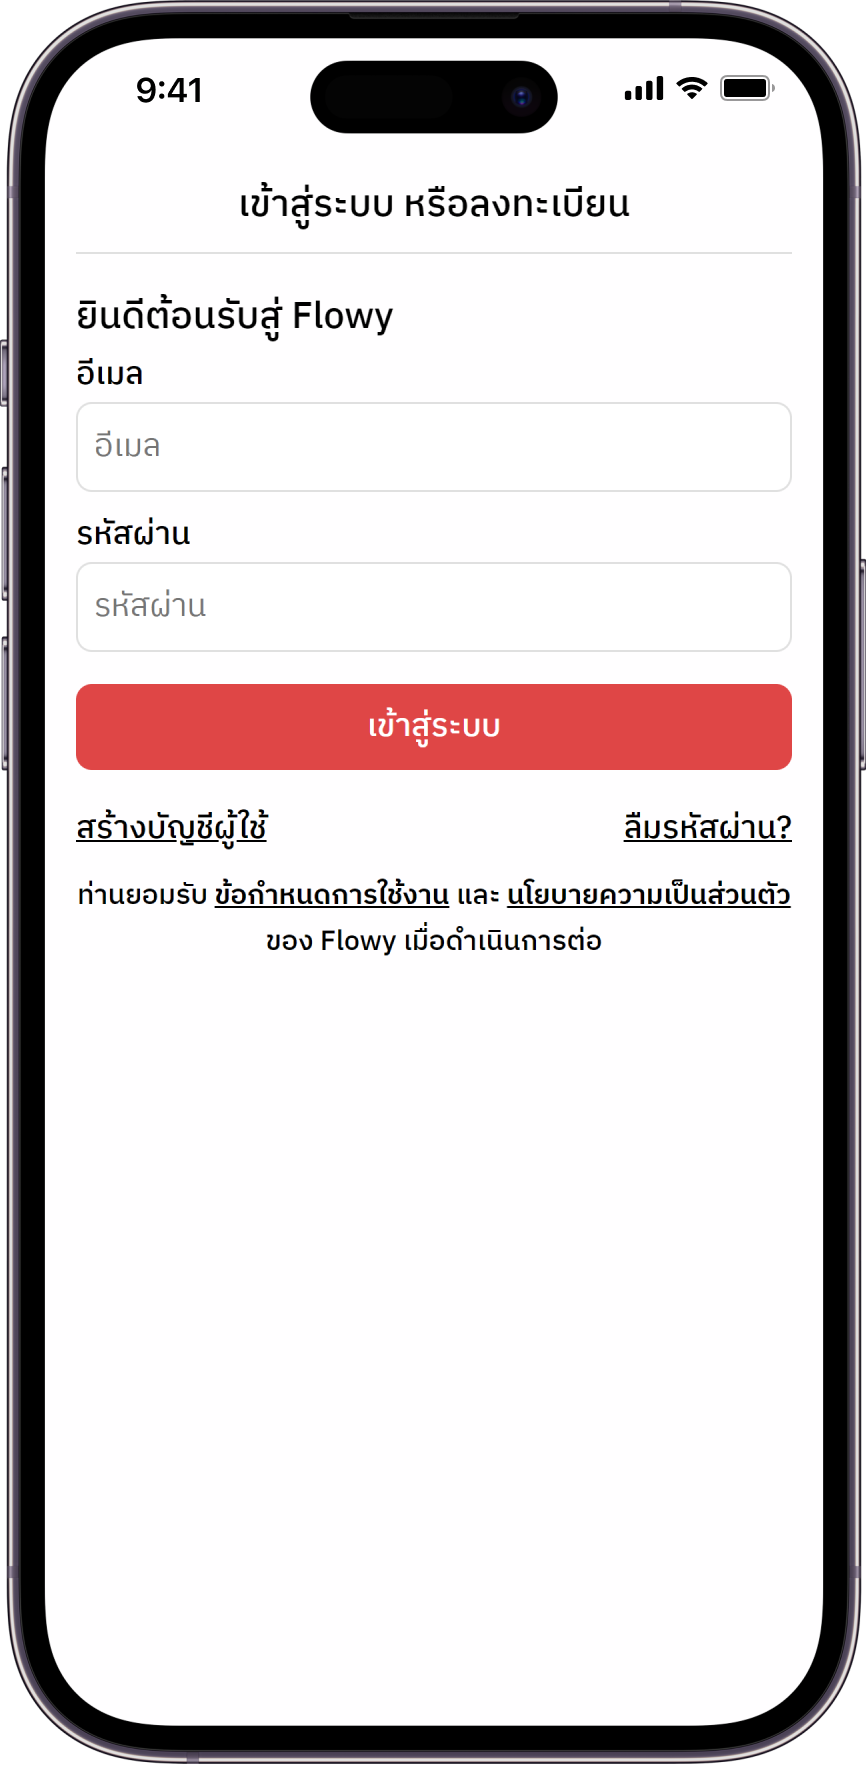
\includegraphics[width=1.9in]{./image/Flowy_login.png}
    \end{center}
    \caption[Flowy login]{หน้าเข้าสู่ระบบสำหรับผู้ใช้งาน (Flowy)}
    \label{fig:Flowy_login}
\end{figure}
\begin{figure}[ht]
    \begin{center}
    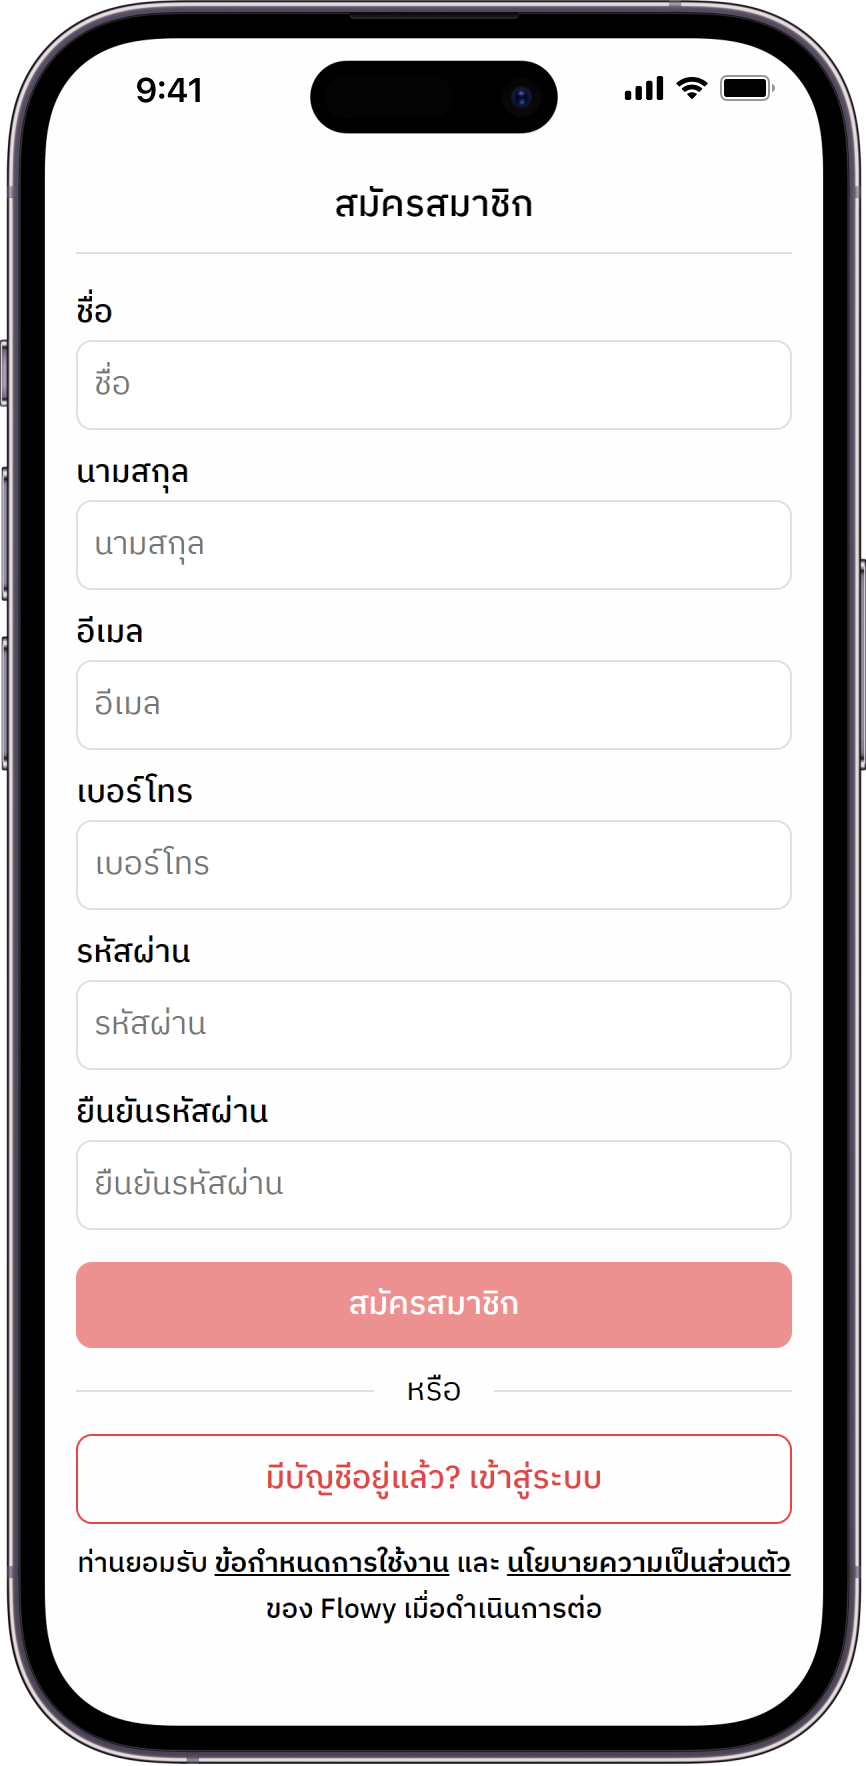
\includegraphics[width=1.9in]{./image/Flowy_register.png}
    \end{center}
    \caption[Flowy register]{หน้าสมัครสมาชิกสำหรับผู้ใช้งาน (Flowy)}
    \label{fig:Flowy_register}
\end{figure}
\begin{figure}[ht]
    \begin{center}
    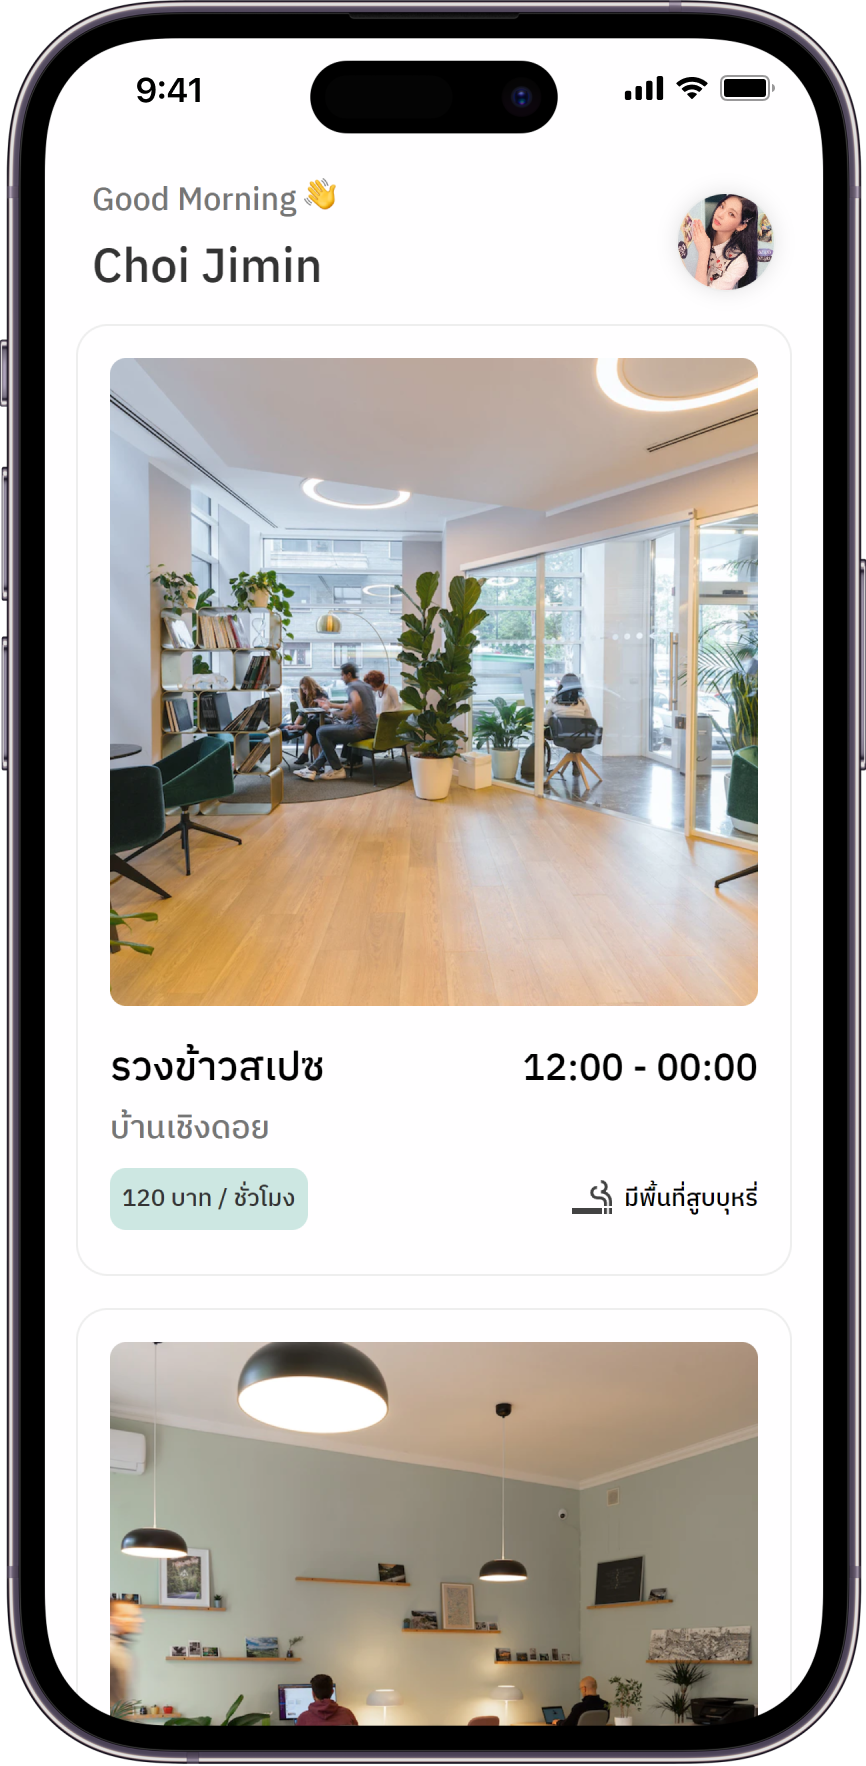
\includegraphics[width=1.9in]{./image/Flowy_explore.png}
    \end{center}
    \caption[Flowy explore]{หน้าแสดงสเปซที่ให้บริการบนแพลตฟอร์ม Flowy}
    \label{fig:Flowy_explore}
\end{figure}
\begin{figure}[ht]
    \begin{center}
    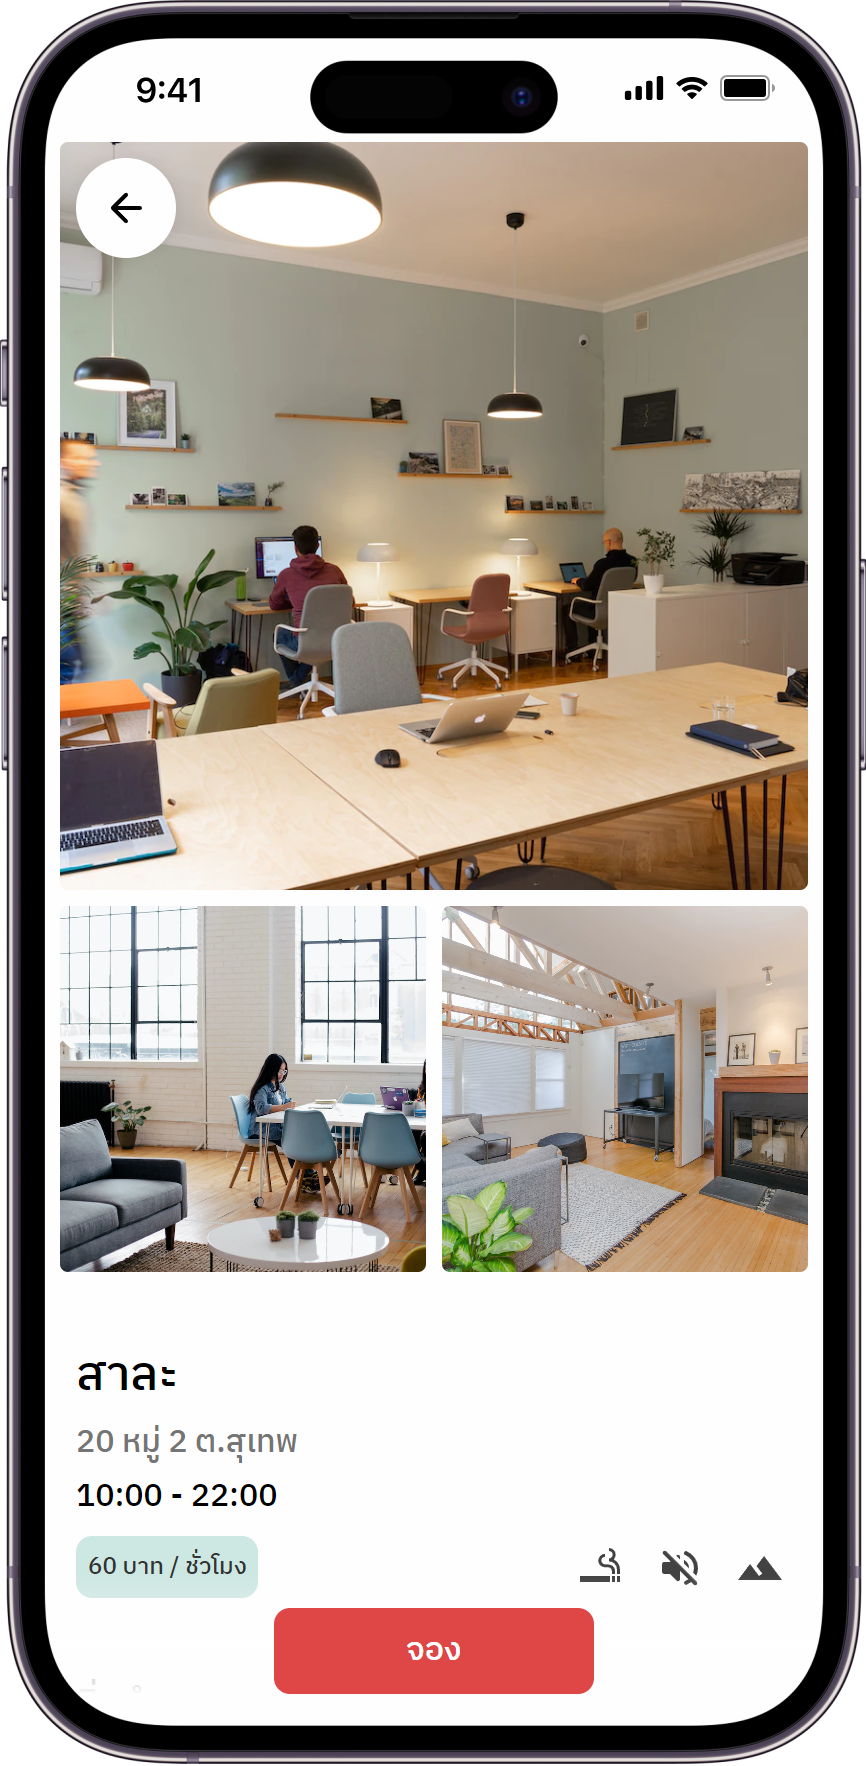
\includegraphics[width=1.9in]{./image/Flowy_info_1.png}
    \end{center}
    \caption[Flowy info 1]{หน้าแสดงรายระเอียดของสเปซ}
    \label{fig:Flowy_info_1}
\end{figure}
\begin{figure}[ht]
    \begin{center}
    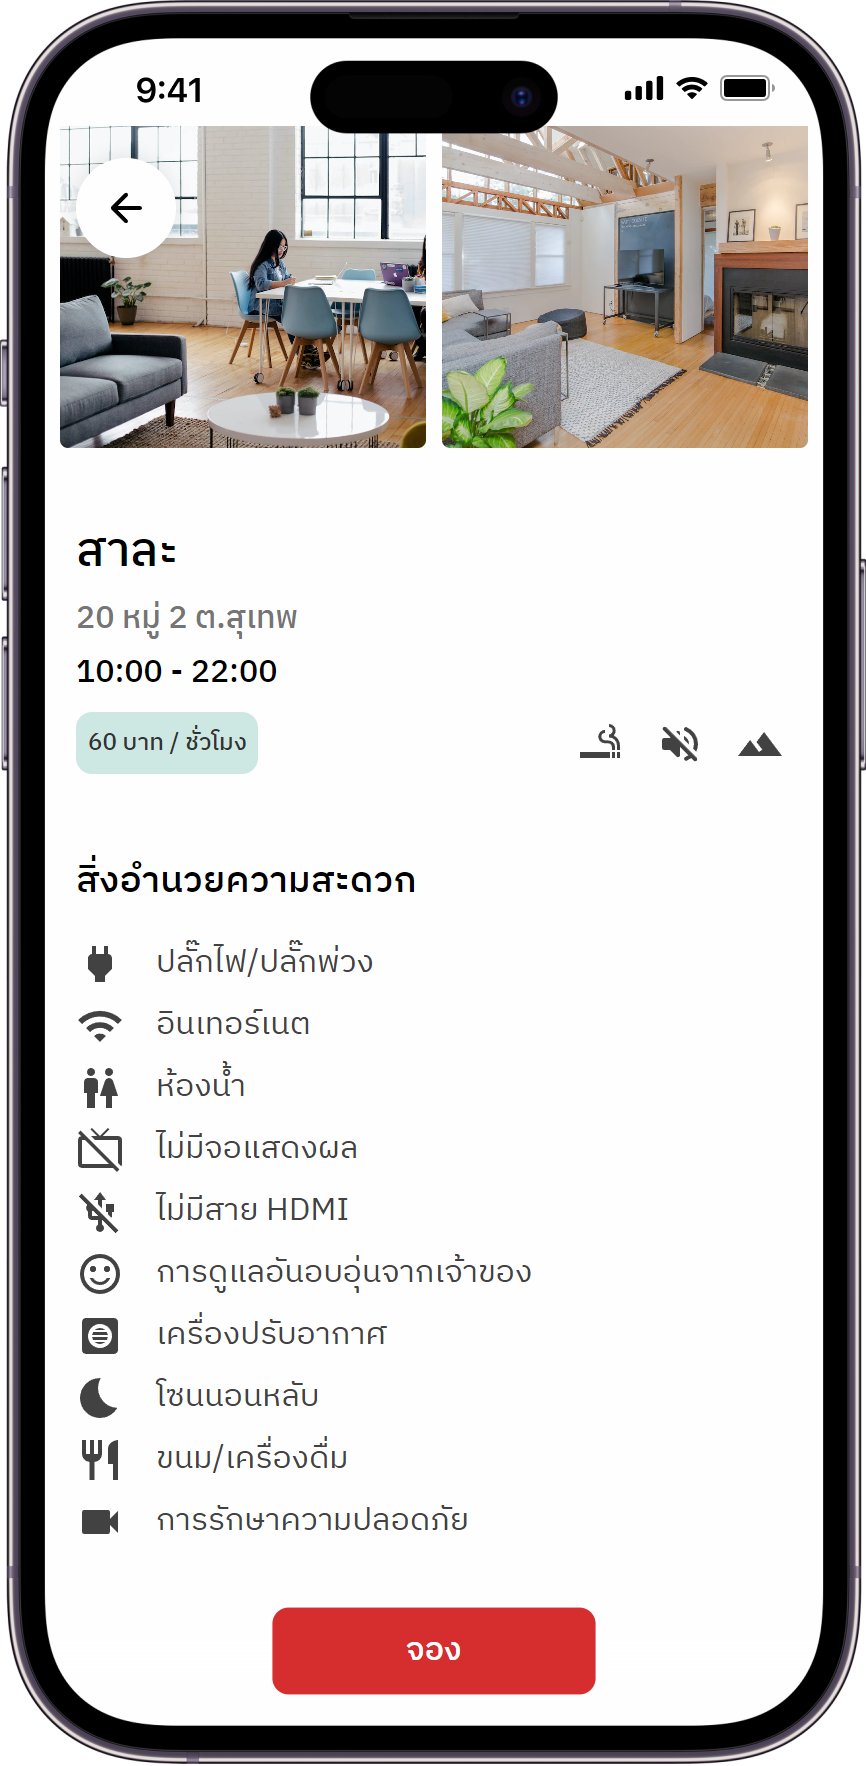
\includegraphics[width=1.9in]{./image/Flowy_info_2.png}
    \end{center}
    \caption[Flowy info 2]{หน้าแสดงรายระเอียดของสเปซ (ต่อ)}
    \label{fig:Flowy_info_2}
\end{figure}
\begin{figure}[ht]
    \begin{center}
    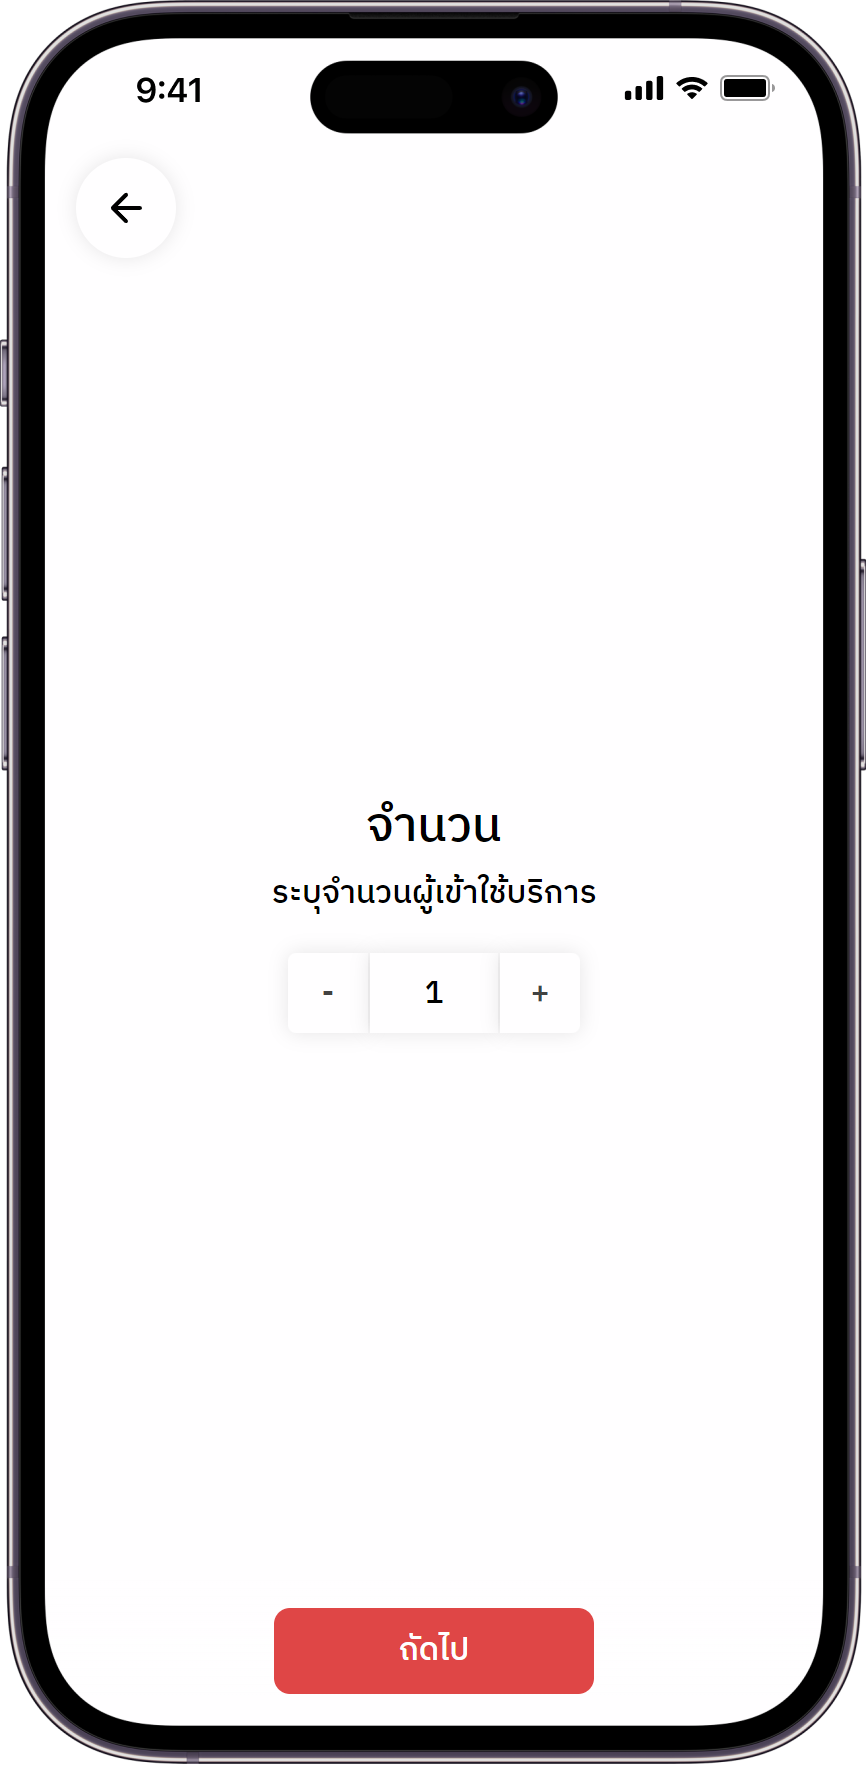
\includegraphics[width=1.9in]{./image/Flowy_book_ctm_amt.png}
    \end{center}
    \caption[Flowy booking customer amount]{หน้าระบุจำนวนผู้เข้าใช้บริการ}
    \label{fig:Flowy_book_ctm_amt}
\end{figure}
\begin{figure}[ht]
    \begin{center}
    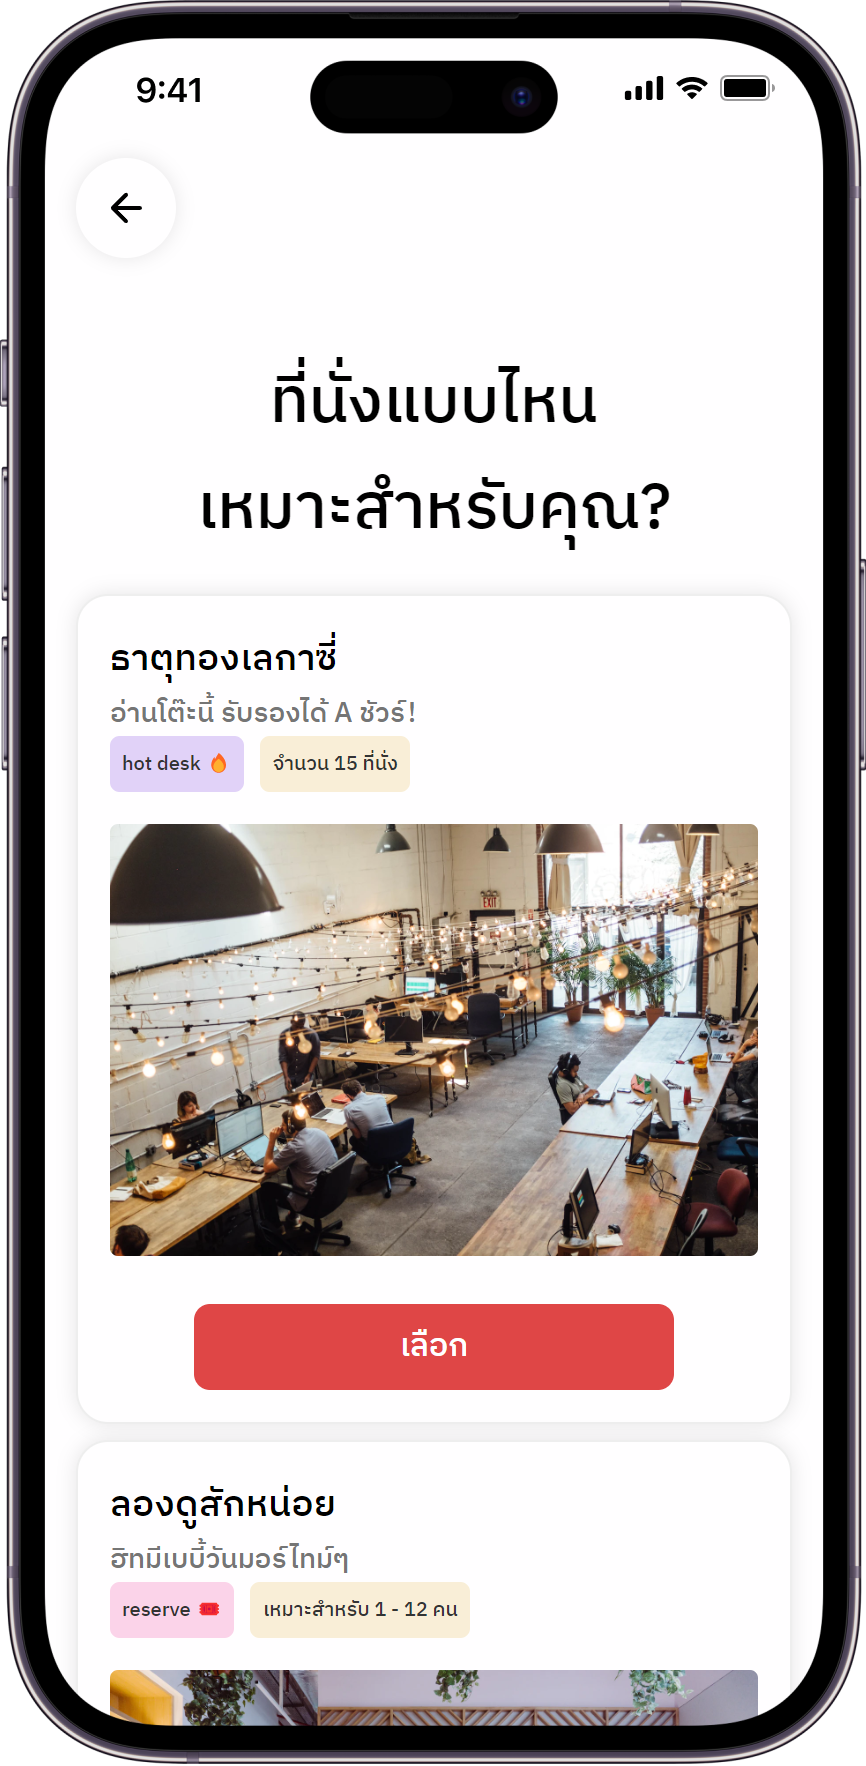
\includegraphics[width=1.9in]{./image/Flowy_book_desk.png}
    \end{center}
    \caption[Flowy booking desk]{หน้าเลือกโต๊ะสำหรับทำกิจกรรมต่าง ๆ}
    \label{fig:Flowy_book_desk}
\end{figure}
\begin{figure}[ht]
    \begin{center}
    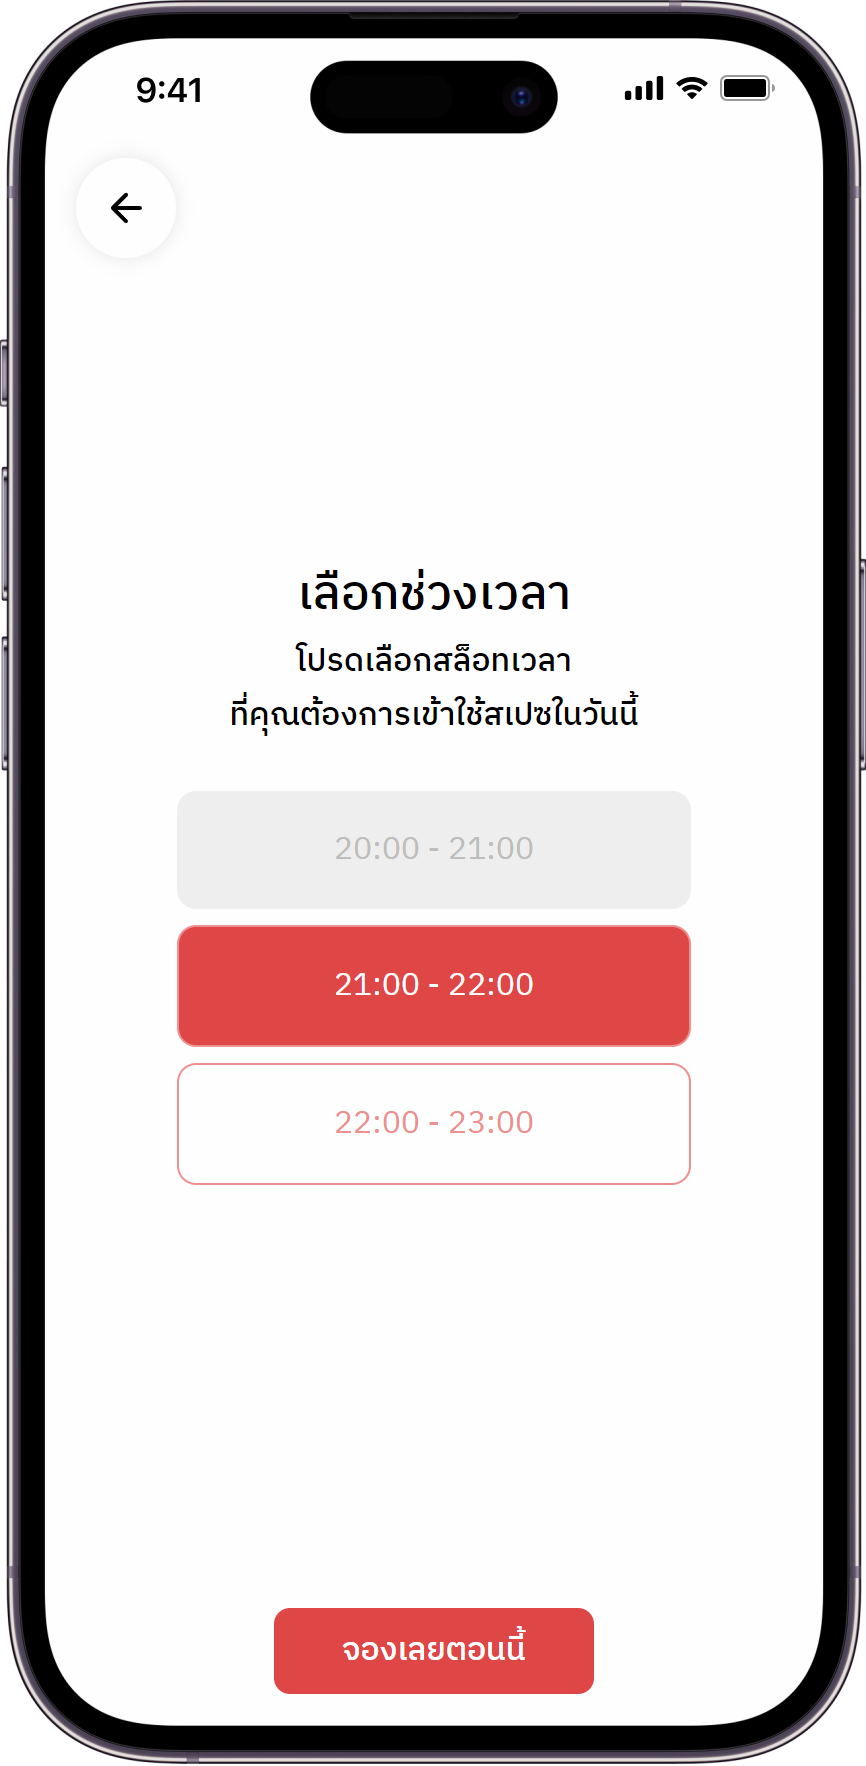
\includegraphics[width=1.9in]{./image/Flowy_book_time_slot.png}
    \end{center}
    \caption[Flowy book time slot]{หน้าระบุเวลาเข้าใช้บริการ}
    \label{fig:Flowy_book_time_slot}
\end{figure}
\begin{figure}[ht]
    \begin{center}
    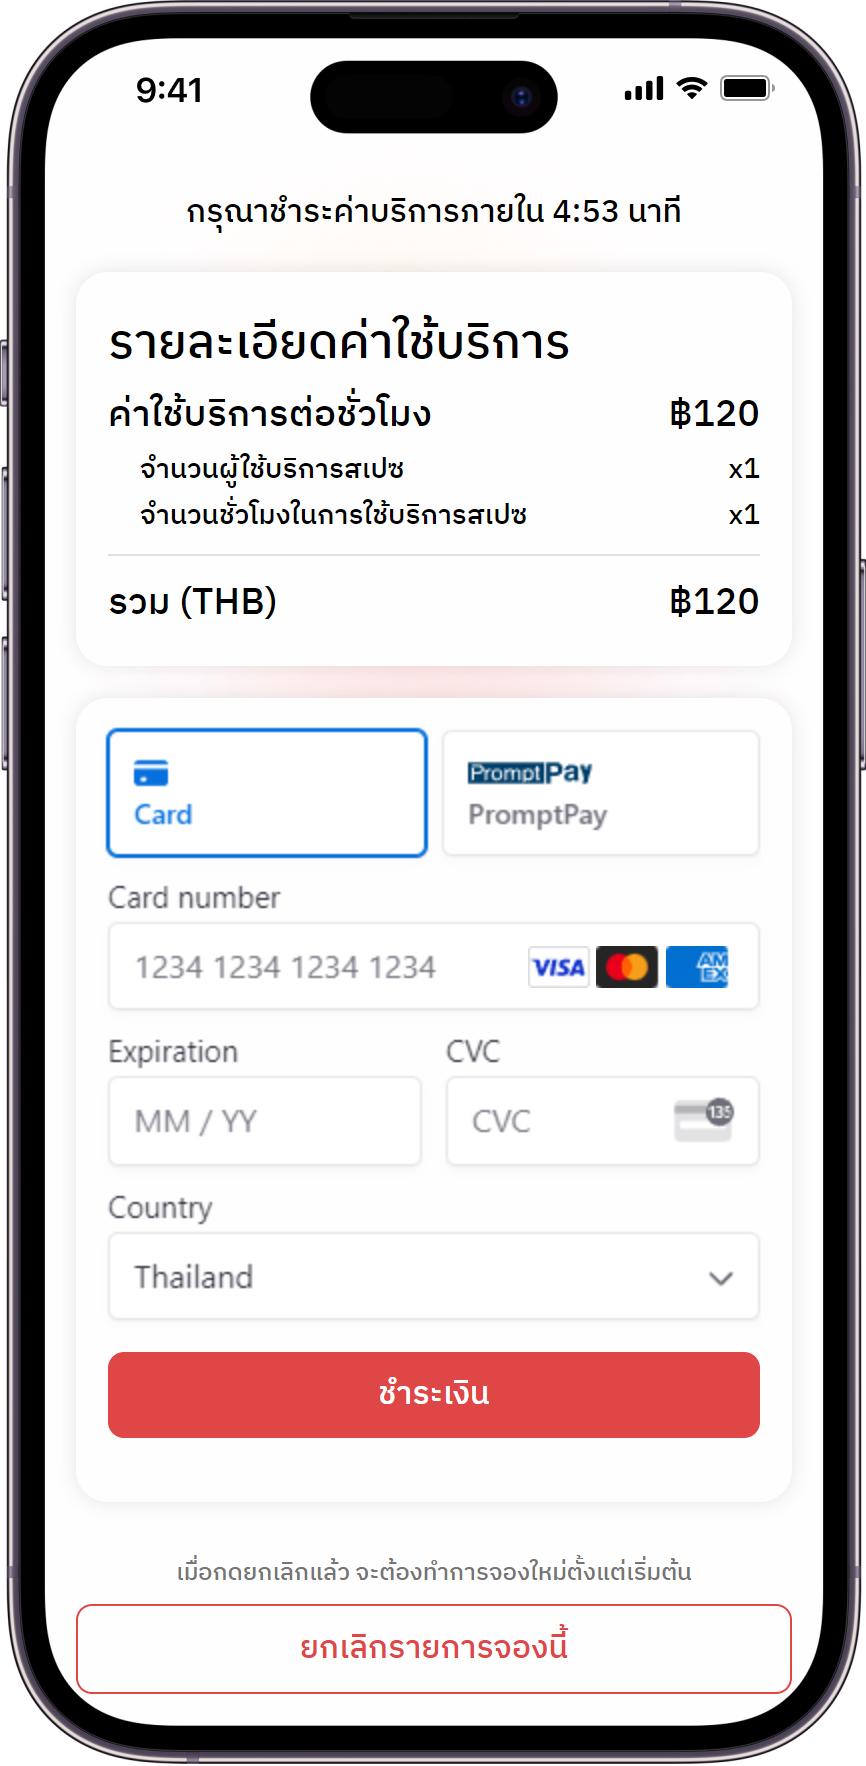
\includegraphics[width=1.9in]{./image/Flowy_payment.png}
    \end{center}
    \caption[Flowy payment]{หน้าชำระค่าบริการ}
    \label{fig:Flowy_payment}
\end{figure}
\begin{figure}[ht]
    \begin{center}
    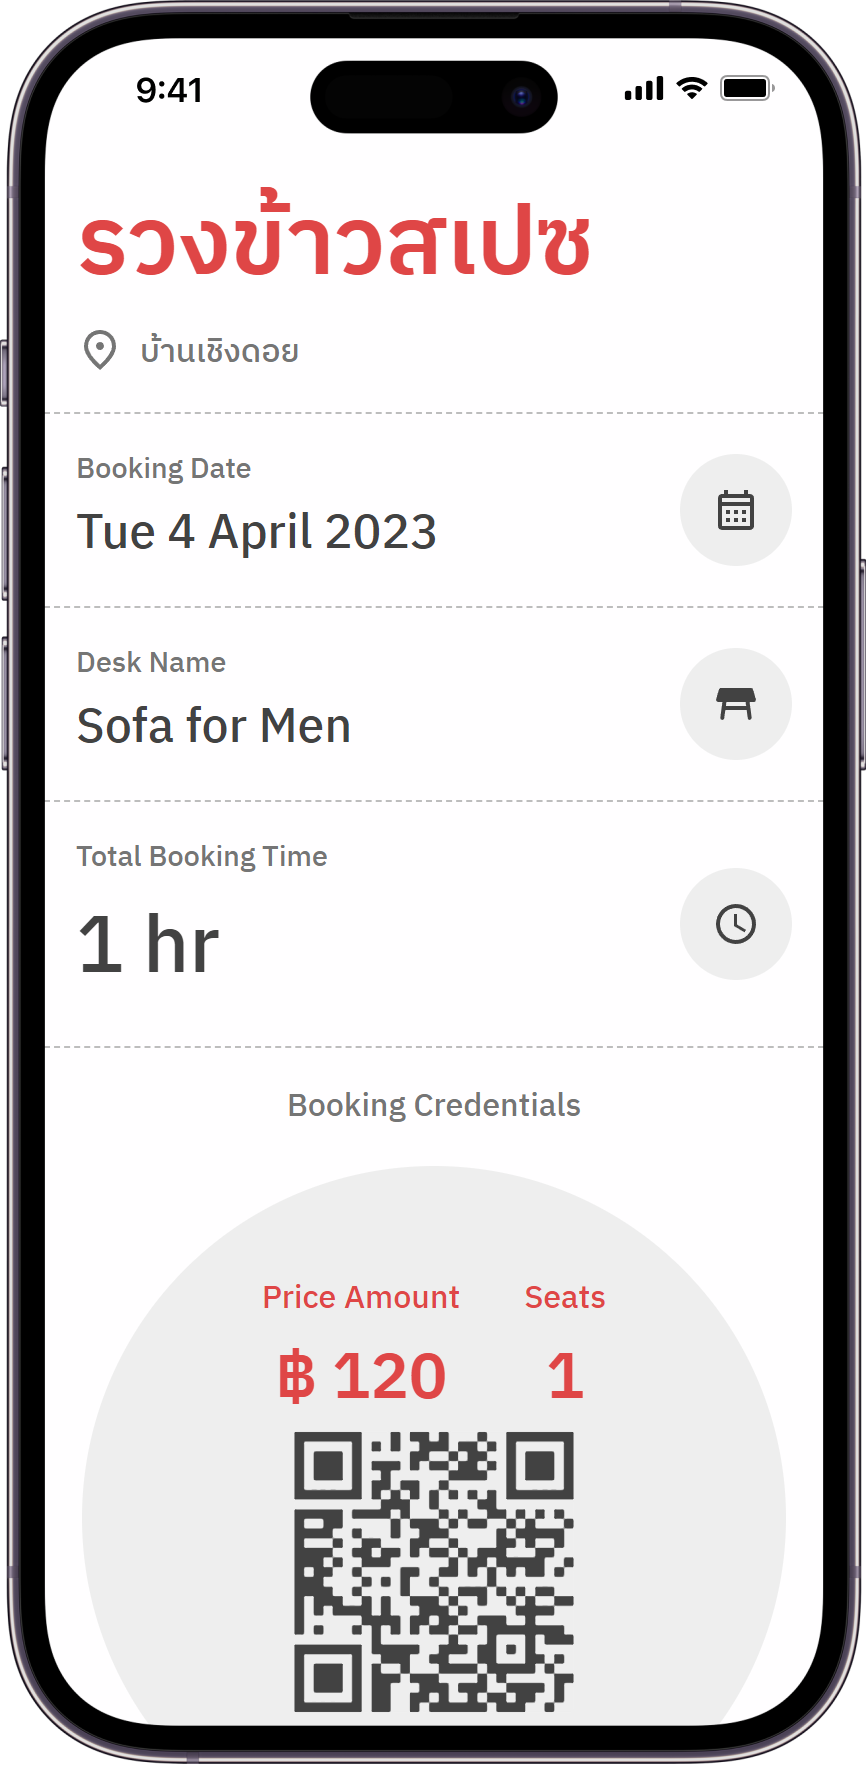
\includegraphics[width=1.9in]{./image/Flowy_ticket_1.png}
    \end{center}
    \caption[Flowy ticket 1]{หน้าแสดงรายระเอียดตั๋ว}
    \label{fig:Flowy_ticket_1}
\end{figure}
\begin{figure}[ht]
    \begin{center}
    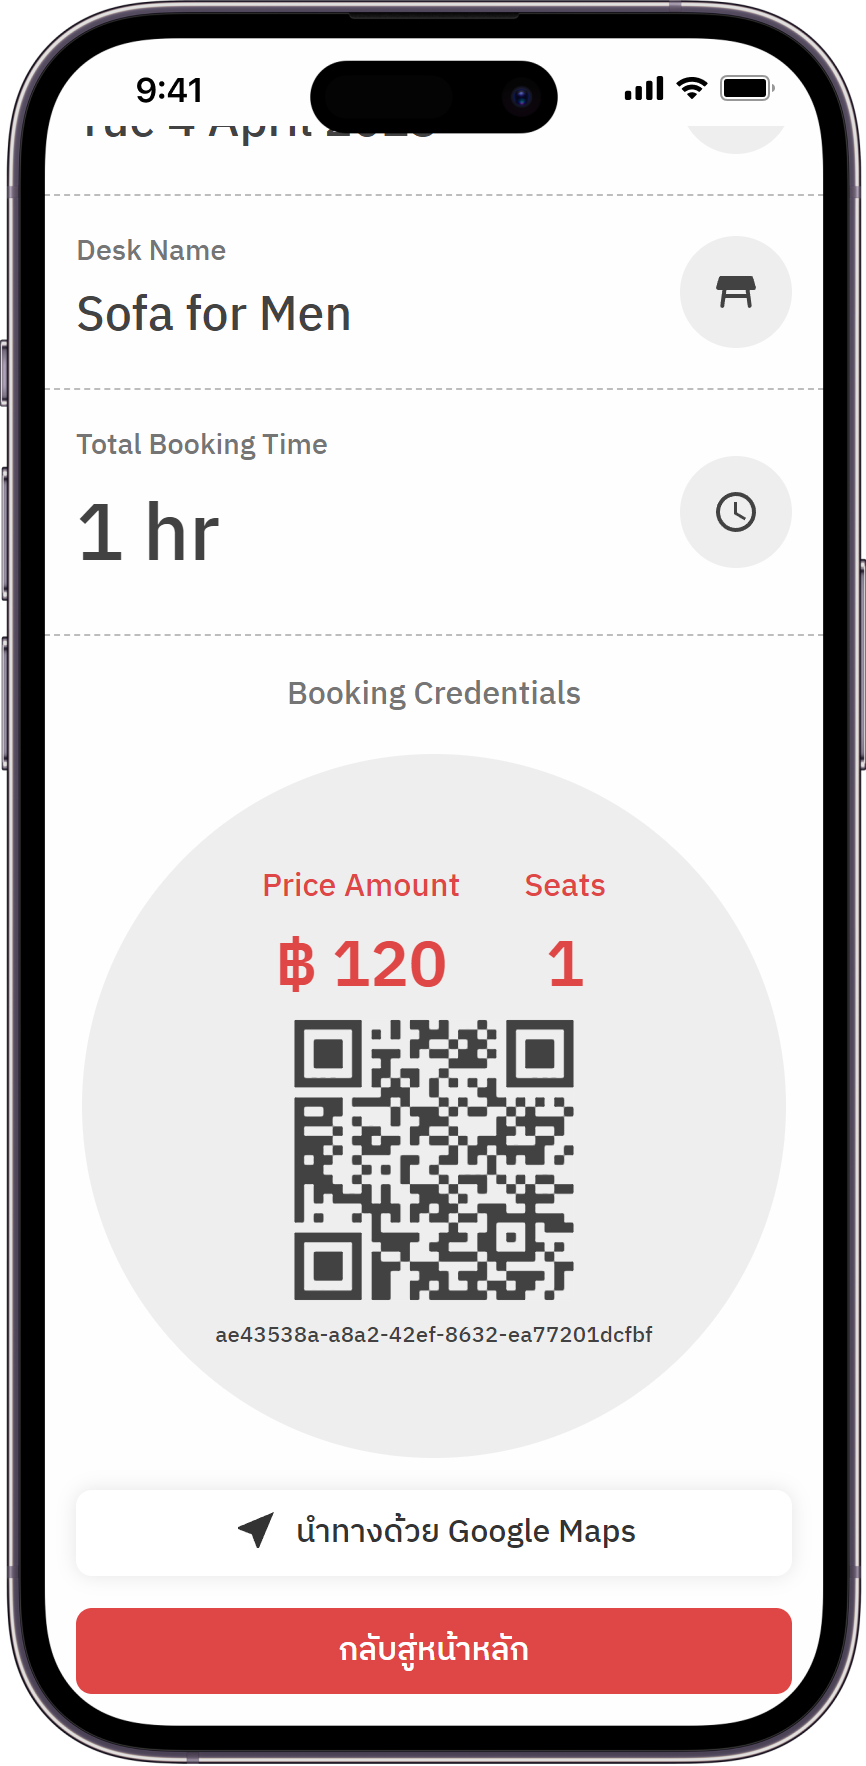
\includegraphics[width=1.9in]{./image/Flowy_ticket_2.png}
    \end{center}
    \caption[Flowy ticket 2]{หน้าแสดงรายระเอียดตั๋ว (ต่อ)}
    \label{fig:Flowy_ticket_2}
\end{figure}
\begin{figure}[ht]
    \begin{center}
    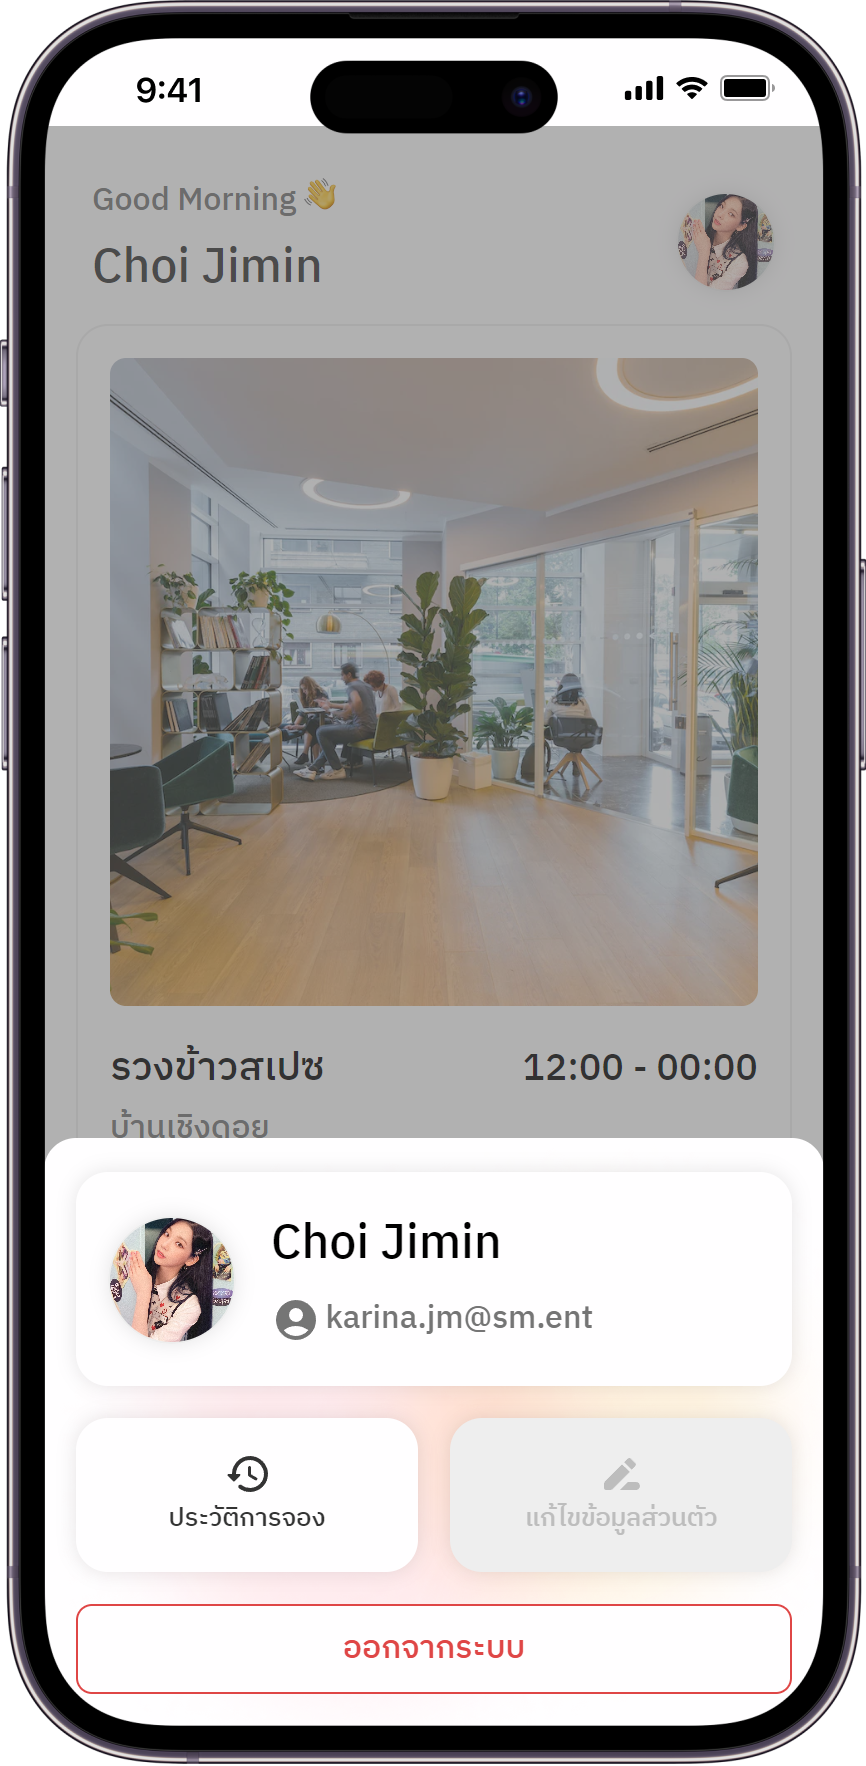
\includegraphics[width=1.9in]{./image/Flowy_account.png}
    \end{center}
    \caption[Flowy account]{หน้าแสดงบัญชีผู้ใช้ (Flowy)}
    \label{fig:Flowy_account}
\end{figure}
\begin{figure}[ht]
    \begin{center}
    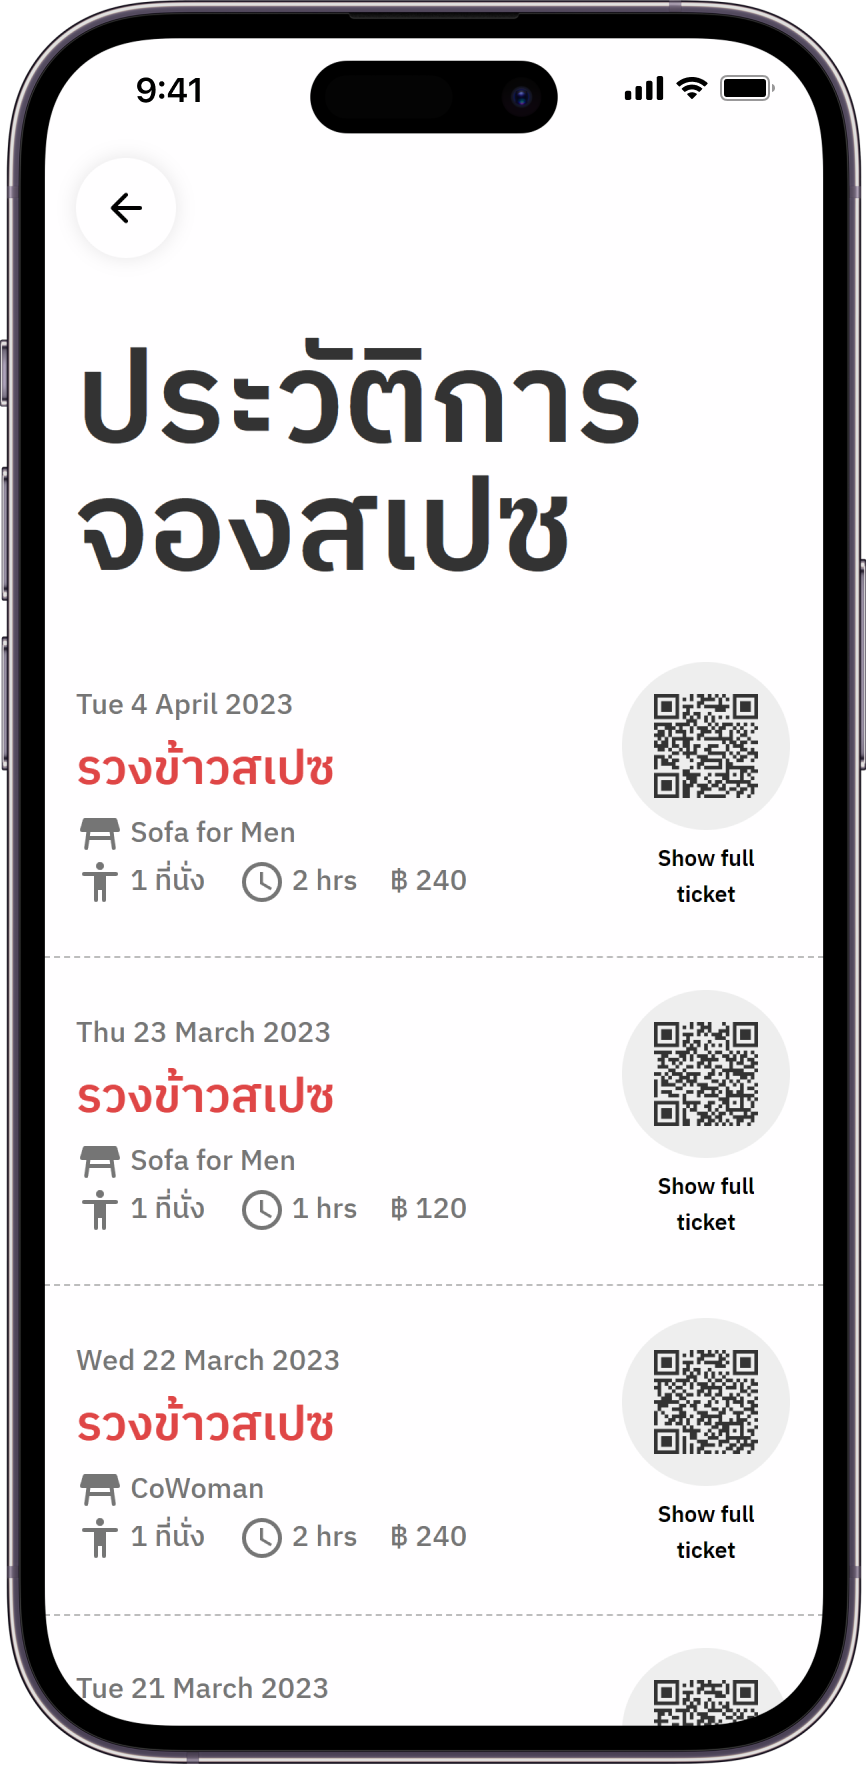
\includegraphics[width=1.9in]{./image/Flowy_book_history.png}
    \end{center}
    \caption[Flowy book history]{หน้าแสดงประวิติการจองสเปซ}
    \label{fig:Flowy_book_history}
\end{figure}
\begin{figure}[ht]
    \begin{center}
    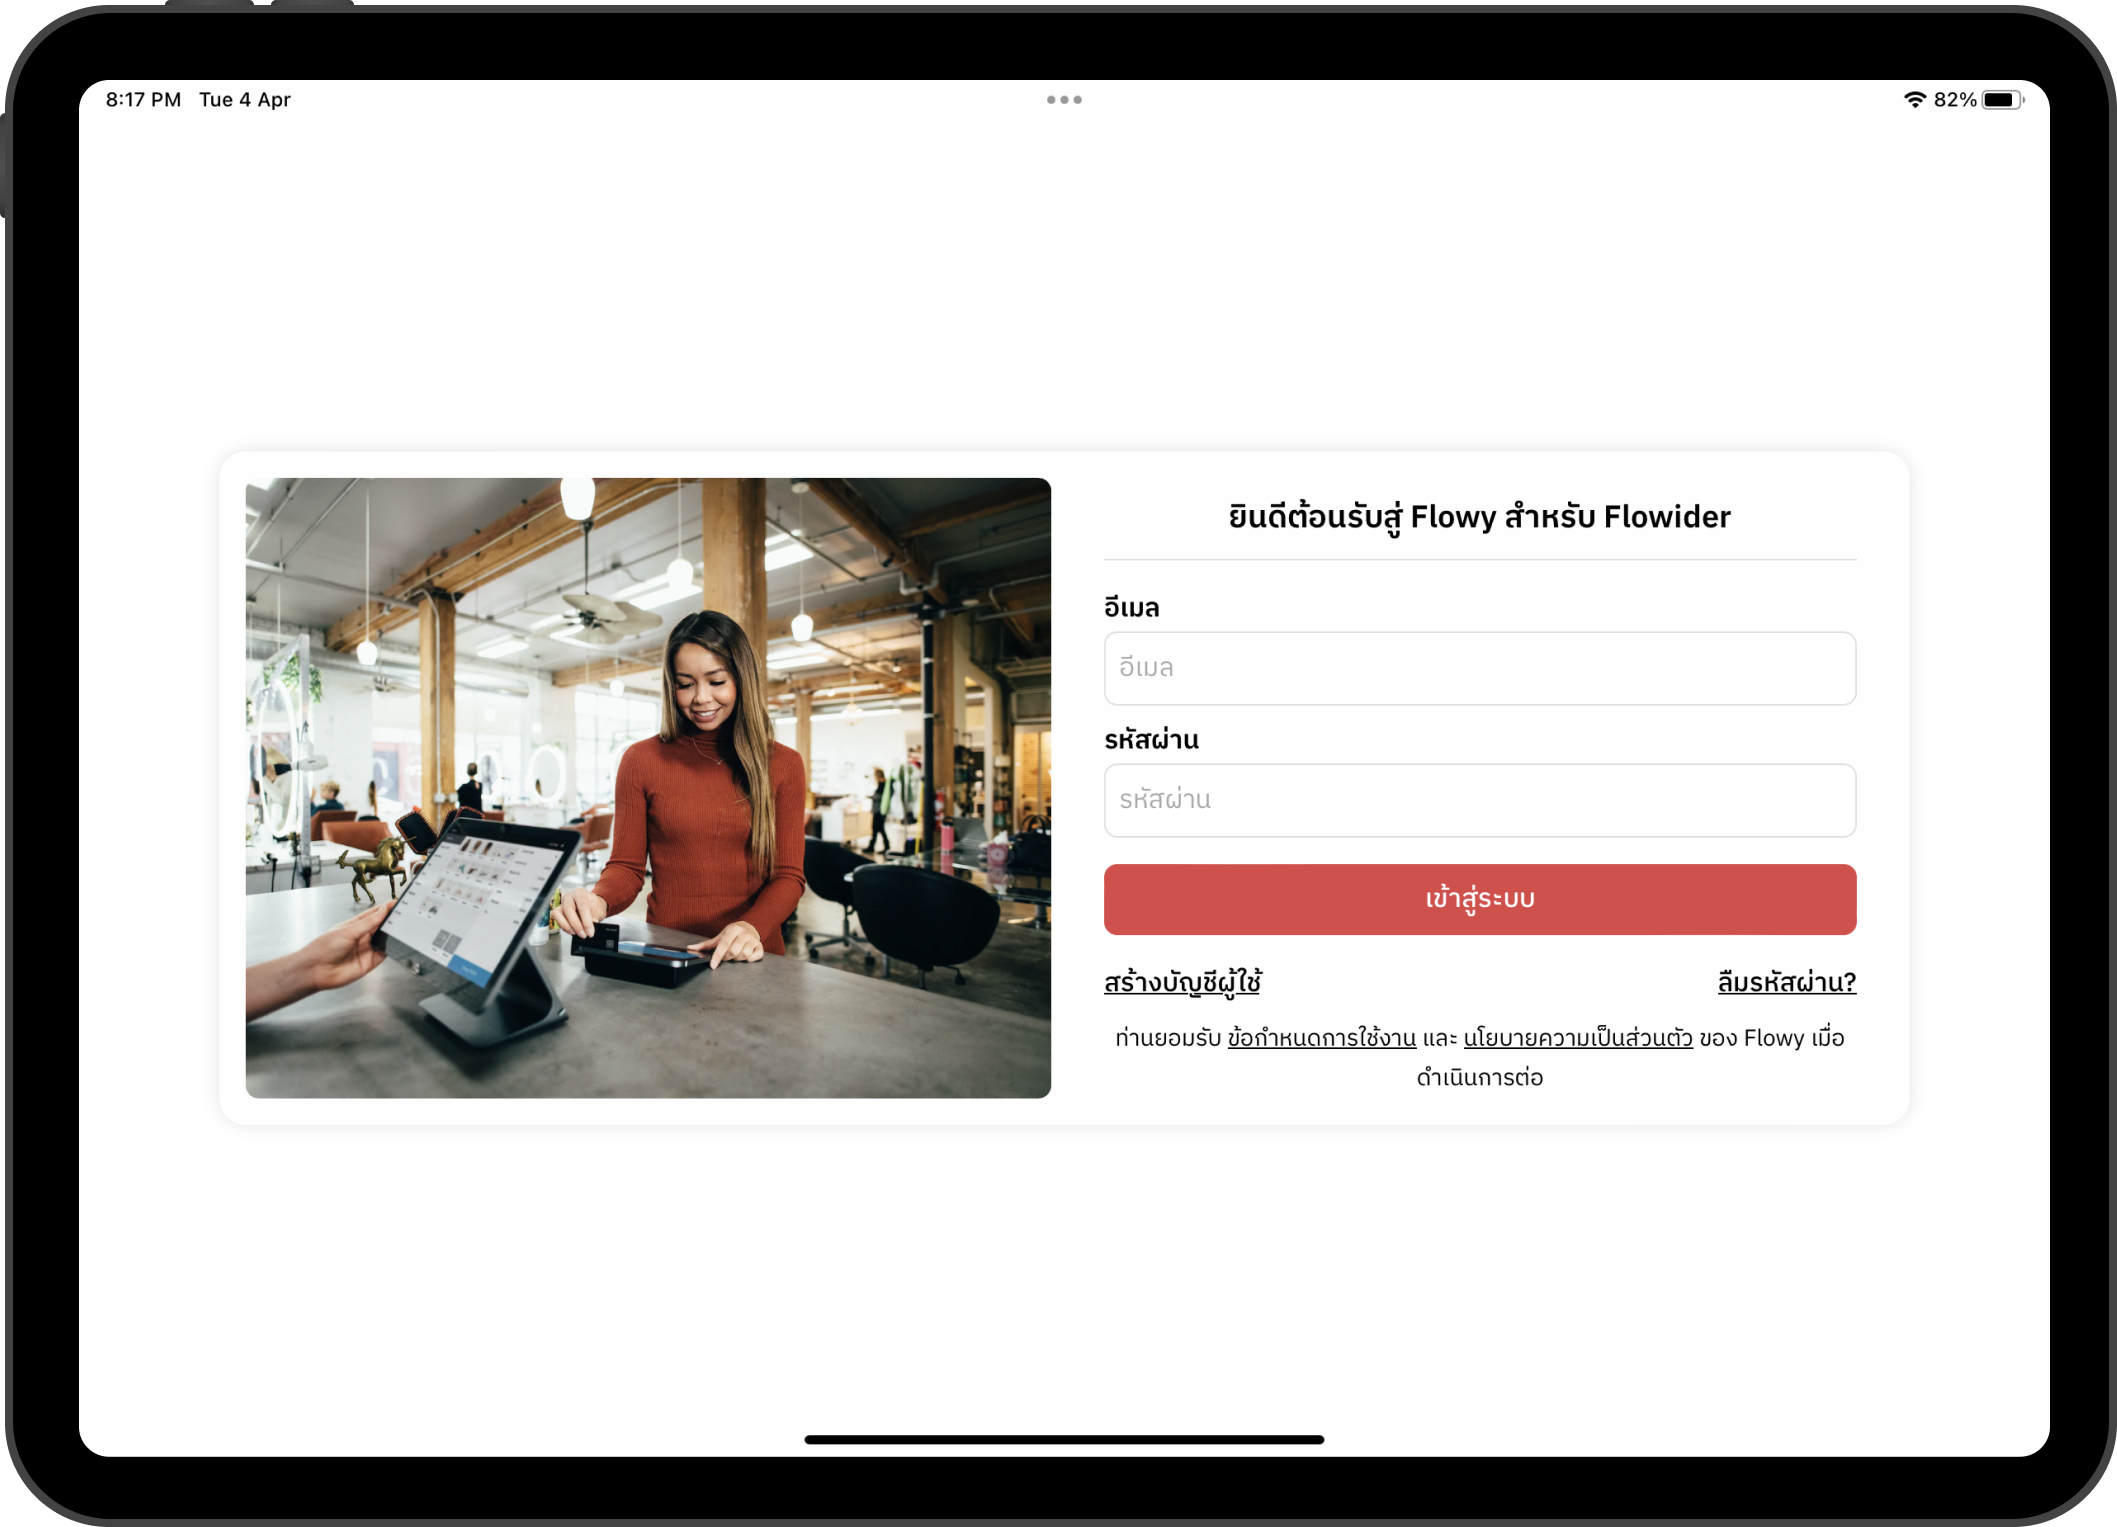
\includegraphics[width=5.5in]{./image/Flowider_login.png}
    \end{center}
    \caption[Flowider login]{หน้าเข้าสู่ระบบสำหรับผู้ใช้งาน (Flowider)}
    \label{fig:Flowider_login}
\end{figure}
\begin{figure}[ht]
    \begin{center}
    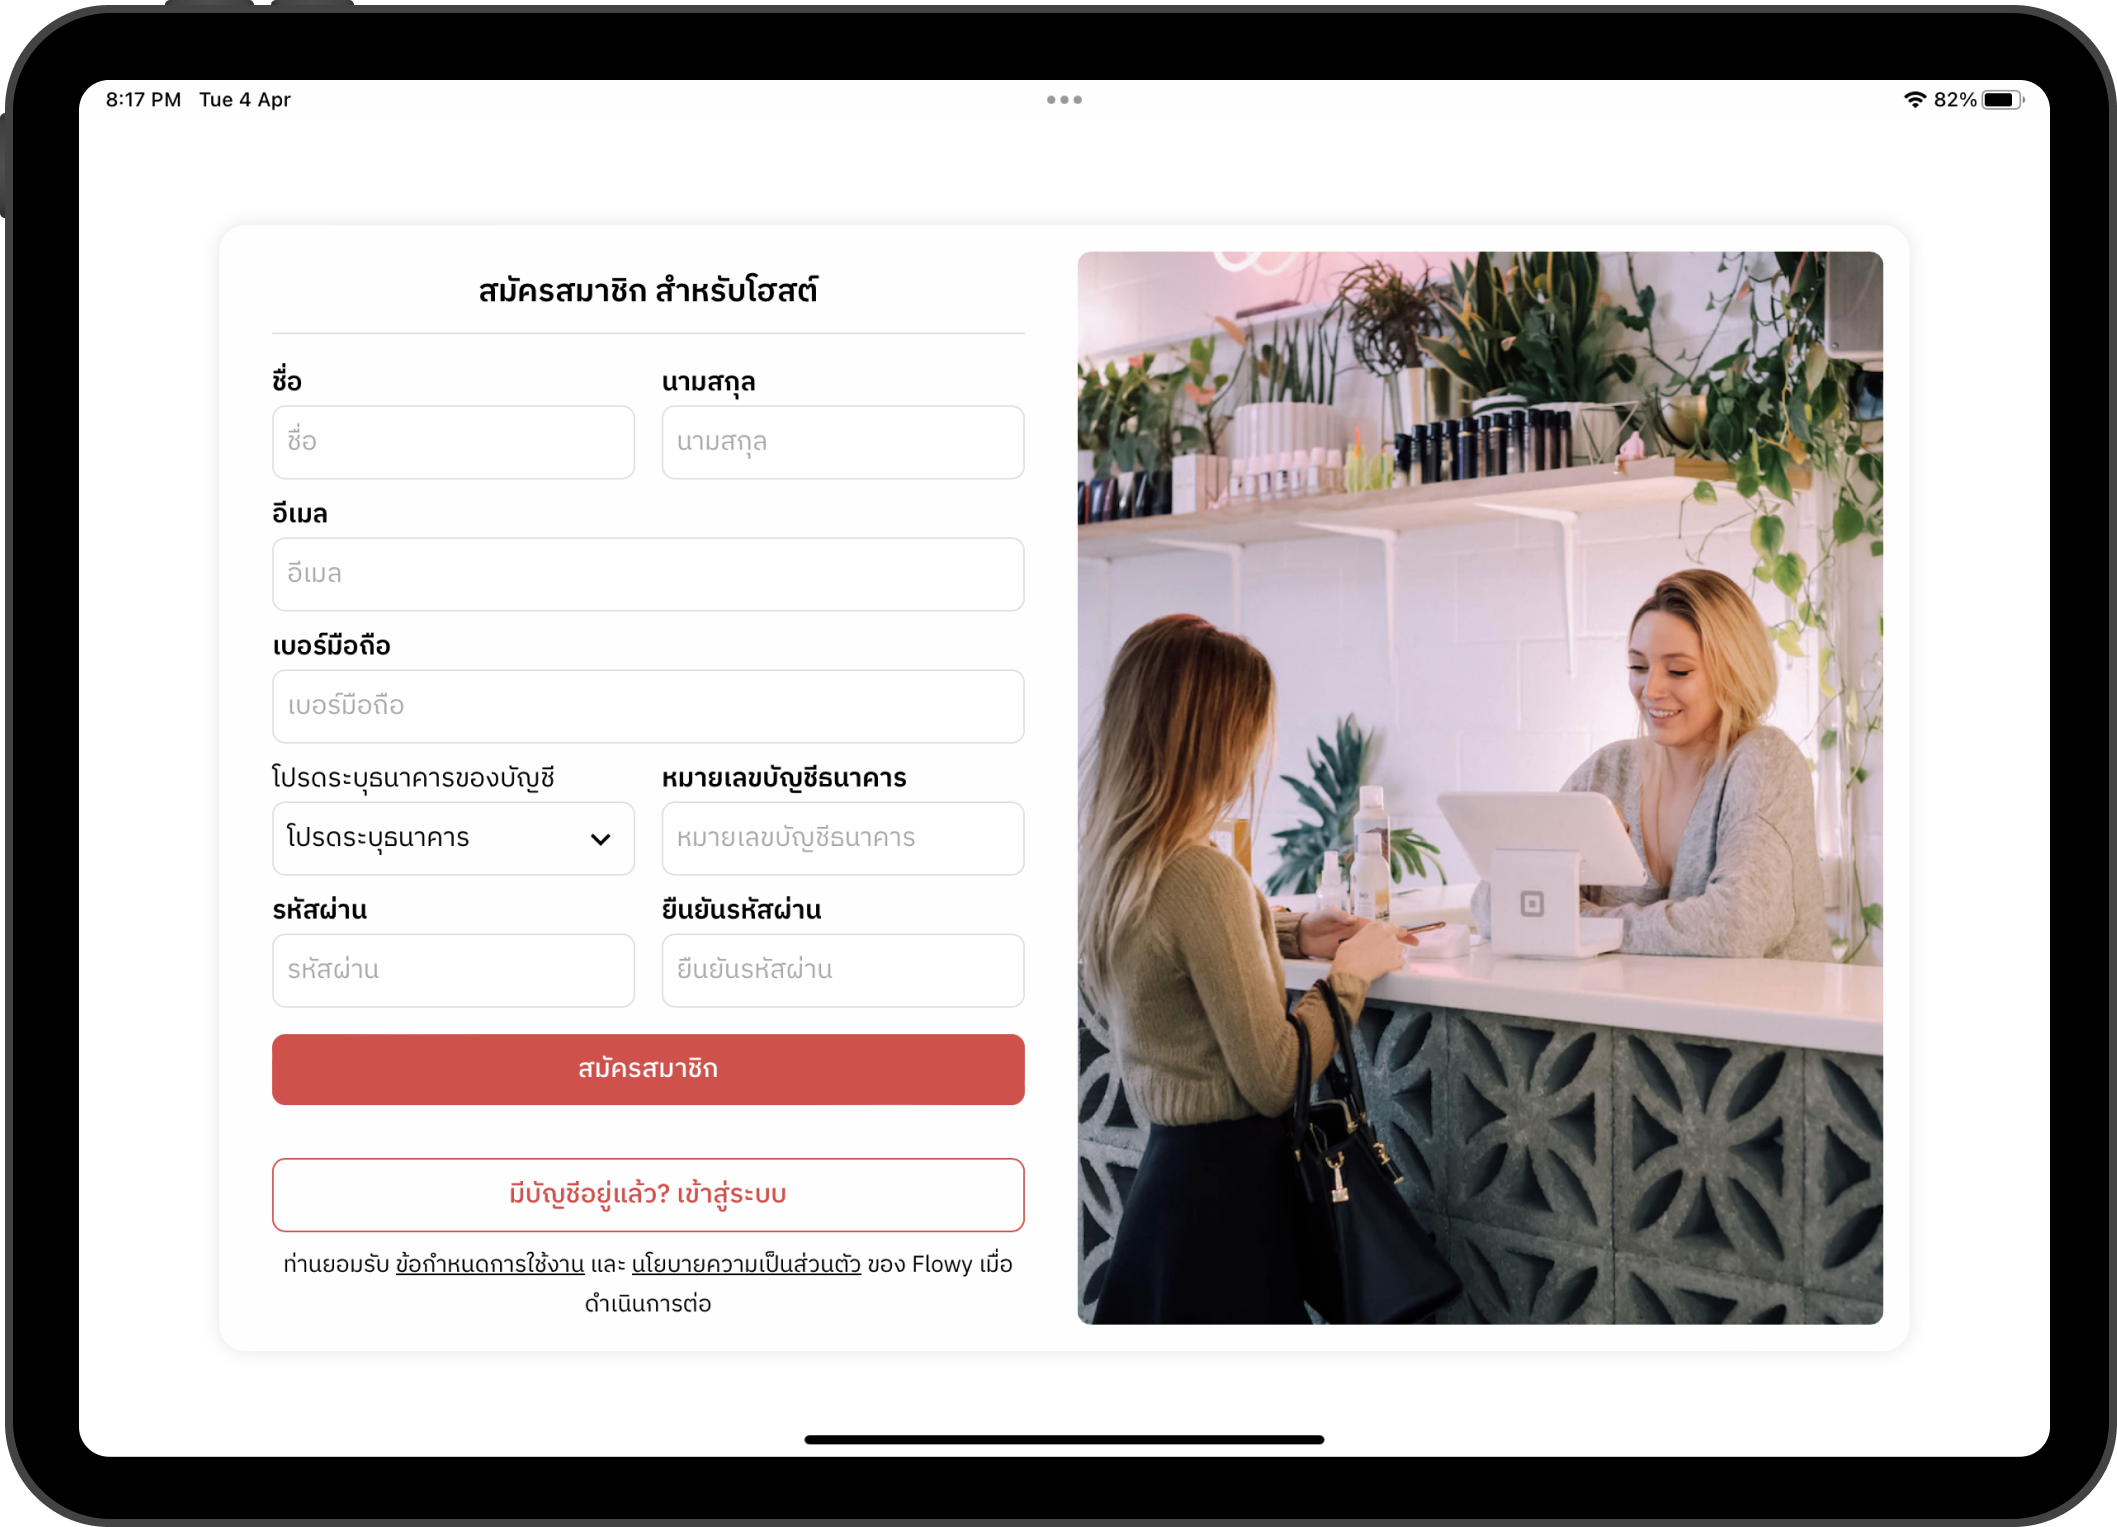
\includegraphics[width=5.5in]{./image/Flowider_register.png}
    \end{center}
    \caption[Flowider register]{หน้าสมัครสมาชิกสำหรับผู้ใช้งาน (Flowider)}
    \label{fig:Flowider_register}
\end{figure}
\begin{figure}[ht]
    \begin{center}
    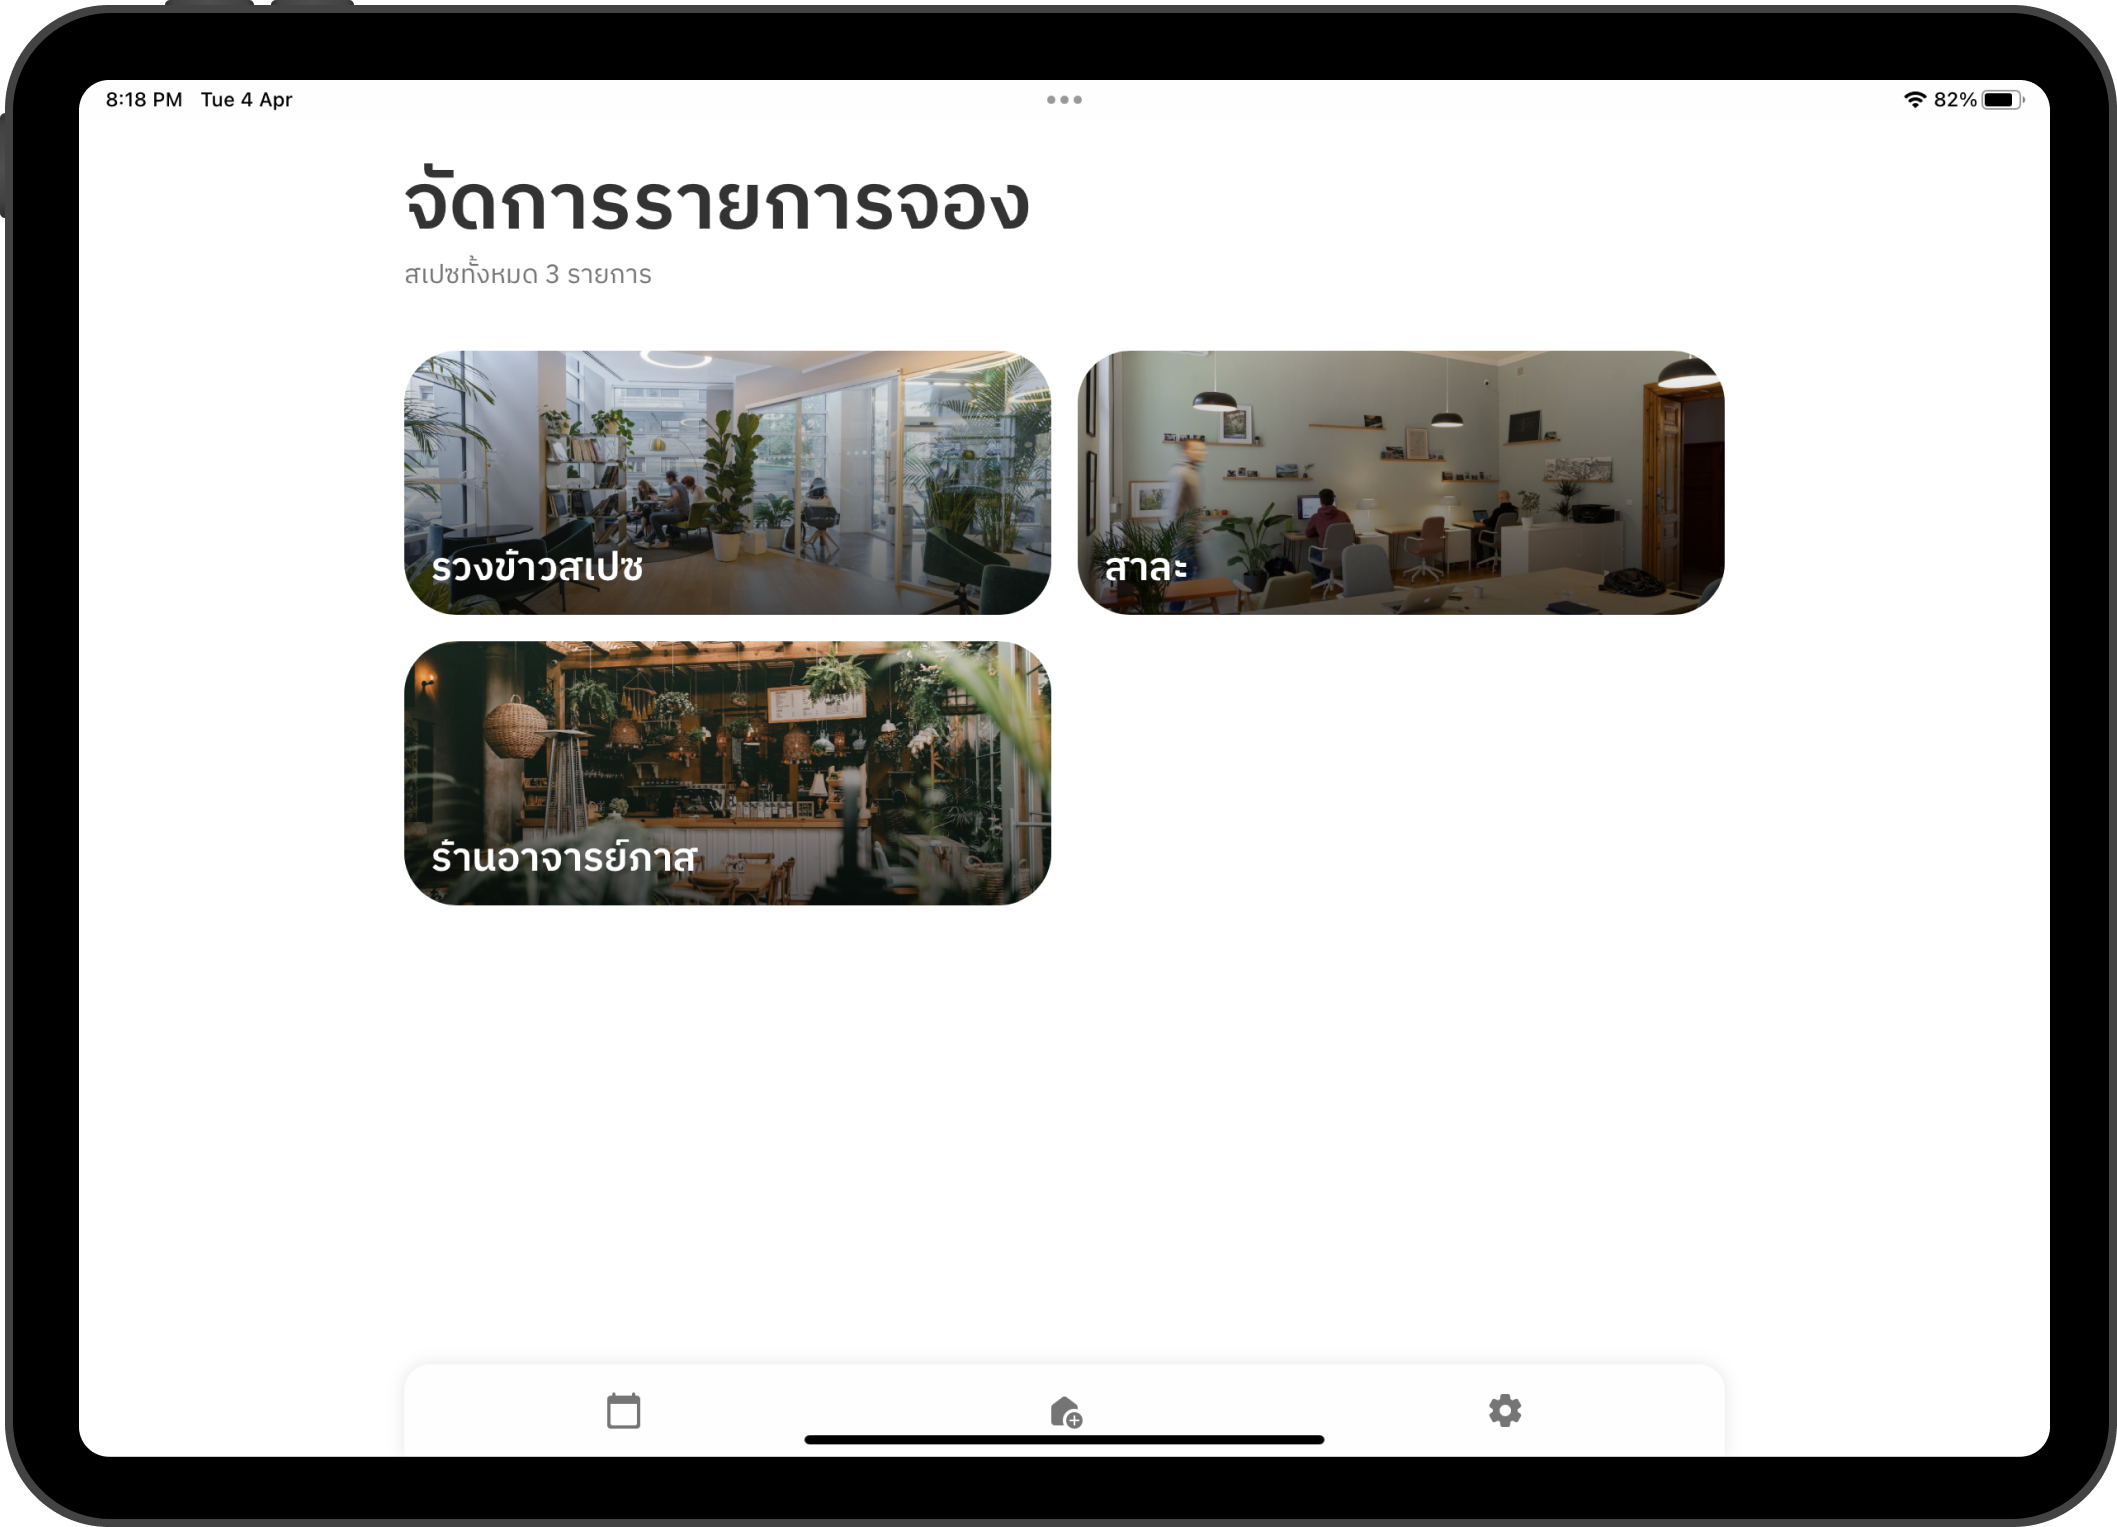
\includegraphics[width=5.5in]{./image/Flowider_booking_mgmt.png}
    \end{center}
    \caption[Flowider booking management]{หน้าจัดการรายการจอง}
    \label{fig:Flowider_booking_mgmt}
\end{figure}
\begin{figure}[ht]
    \begin{center}
    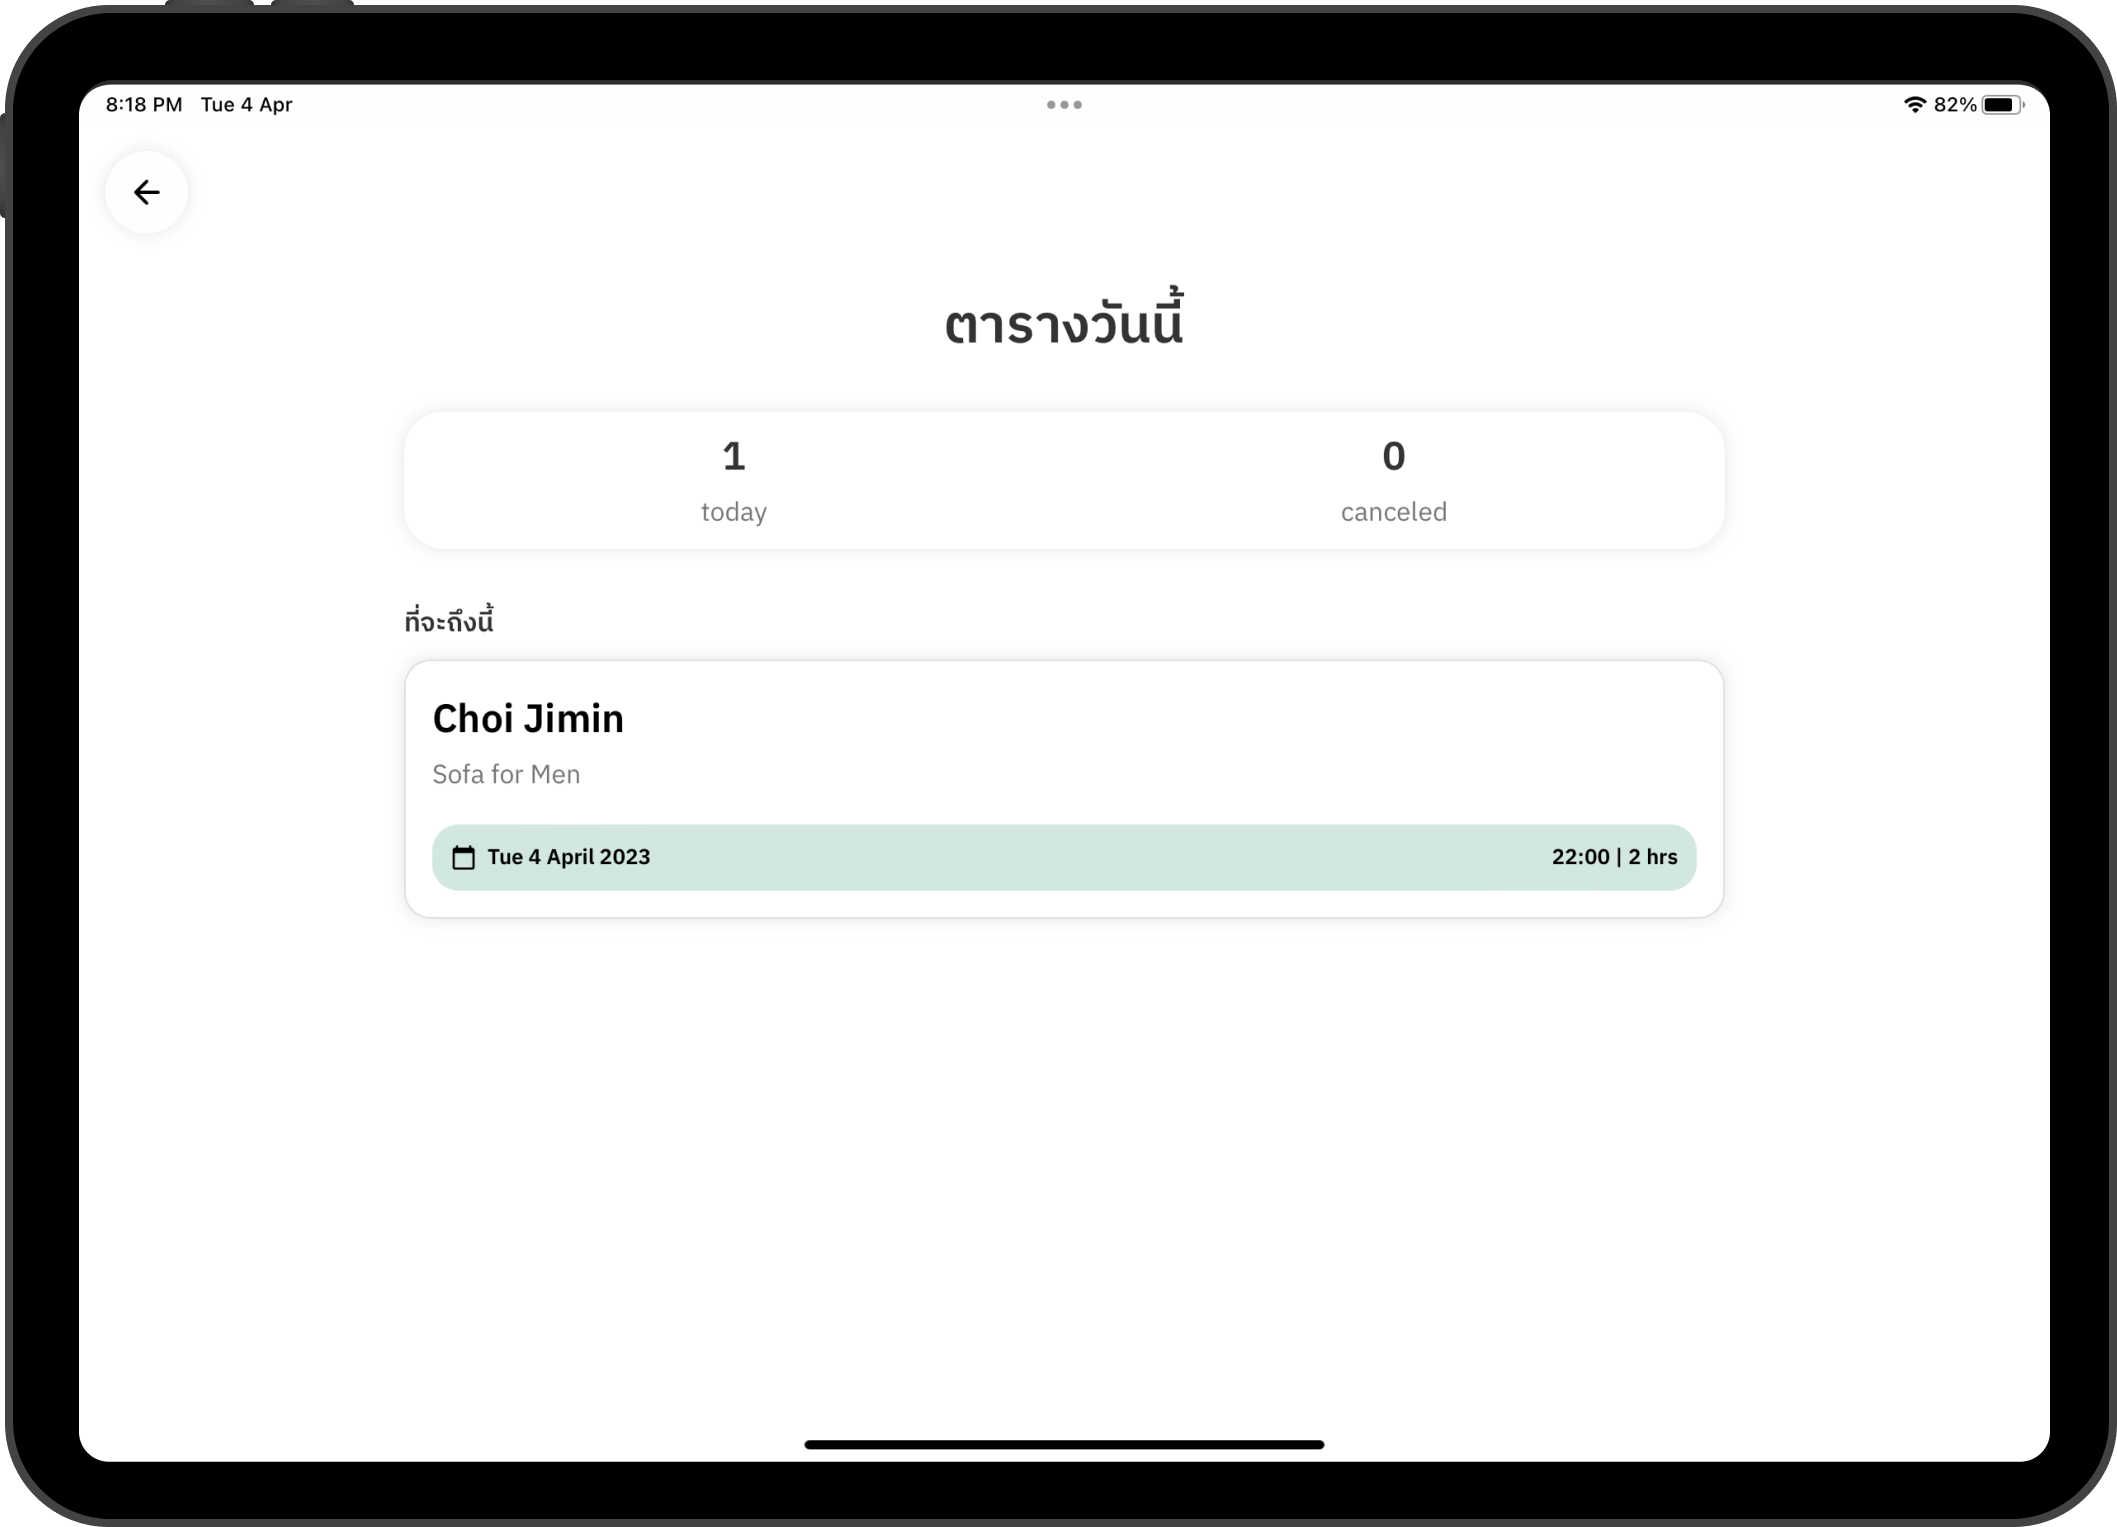
\includegraphics[width=5.5in]{./image/Flowider_schedule.png}
    \end{center}
    \caption[Flowide schedule]{หน้าแสดงรายระเอียดการจองของแต่ละสเปซ}
    \label{fig:Flowider_schedule}
\end{figure}
\begin{figure}[ht]
    \begin{center}
    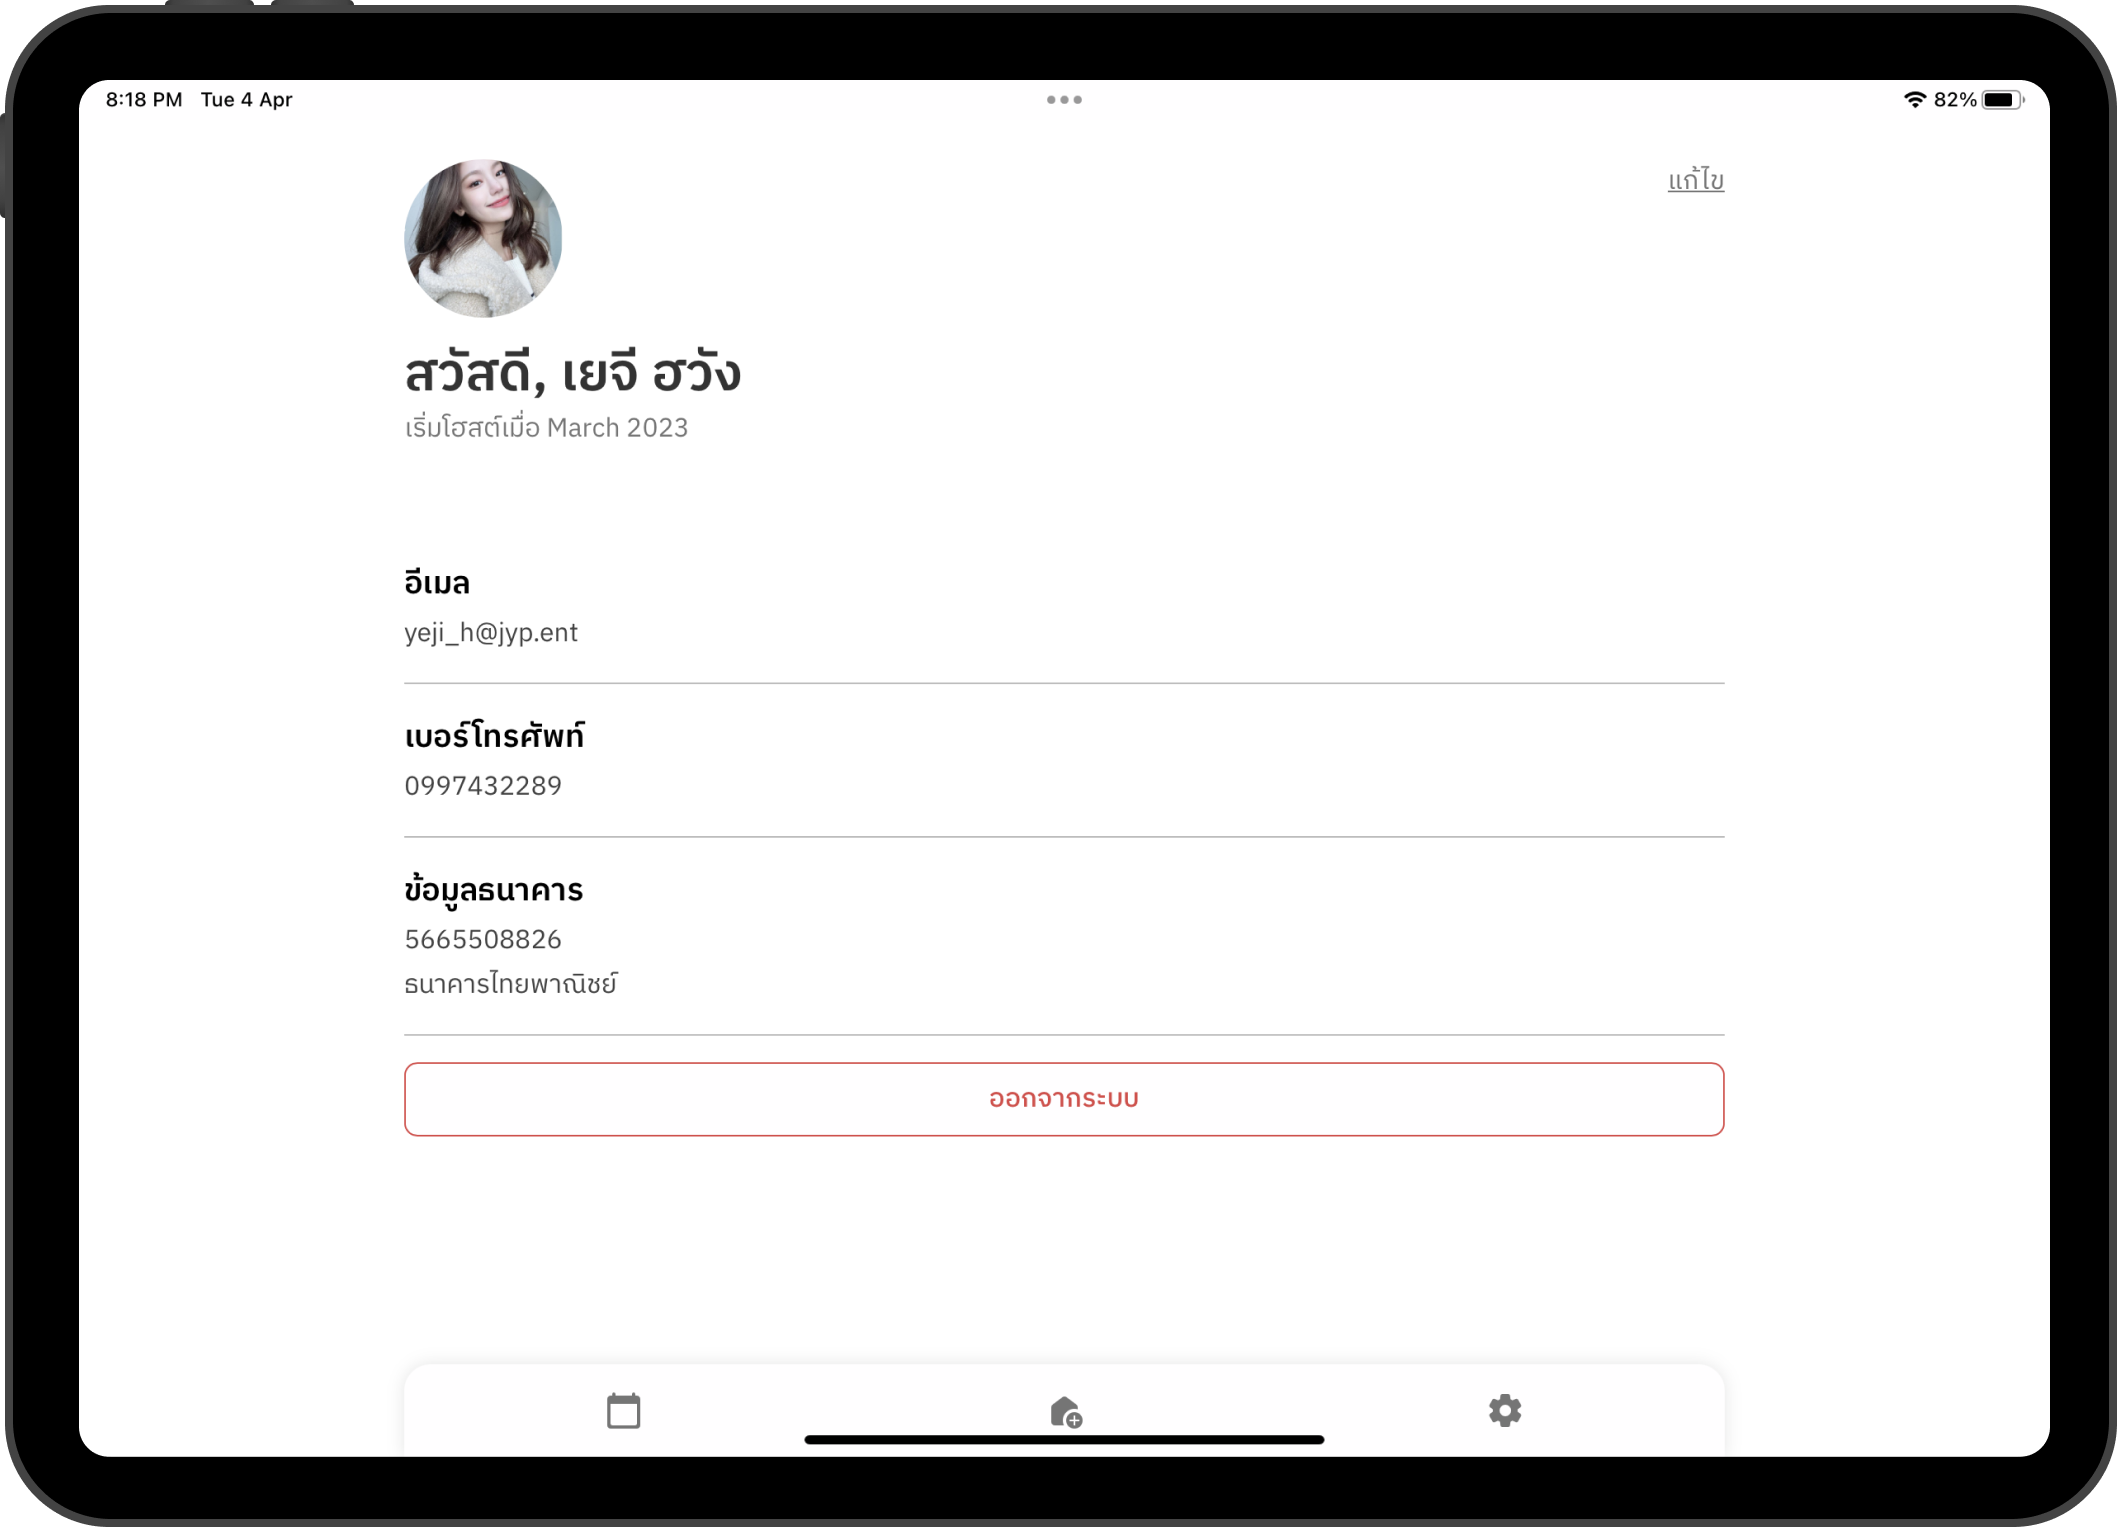
\includegraphics[width=5.5in]{./image/Flowider_account.png}
    \end{center}
    \caption[Flowider account]{หน้าแสดงบัญชีผู้ใช้ของผู้ใช้บริการ (Flowider)}
    \label{fig:Flowider_account}
\end{figure}
\begin{figure}[ht]
    \begin{center}
    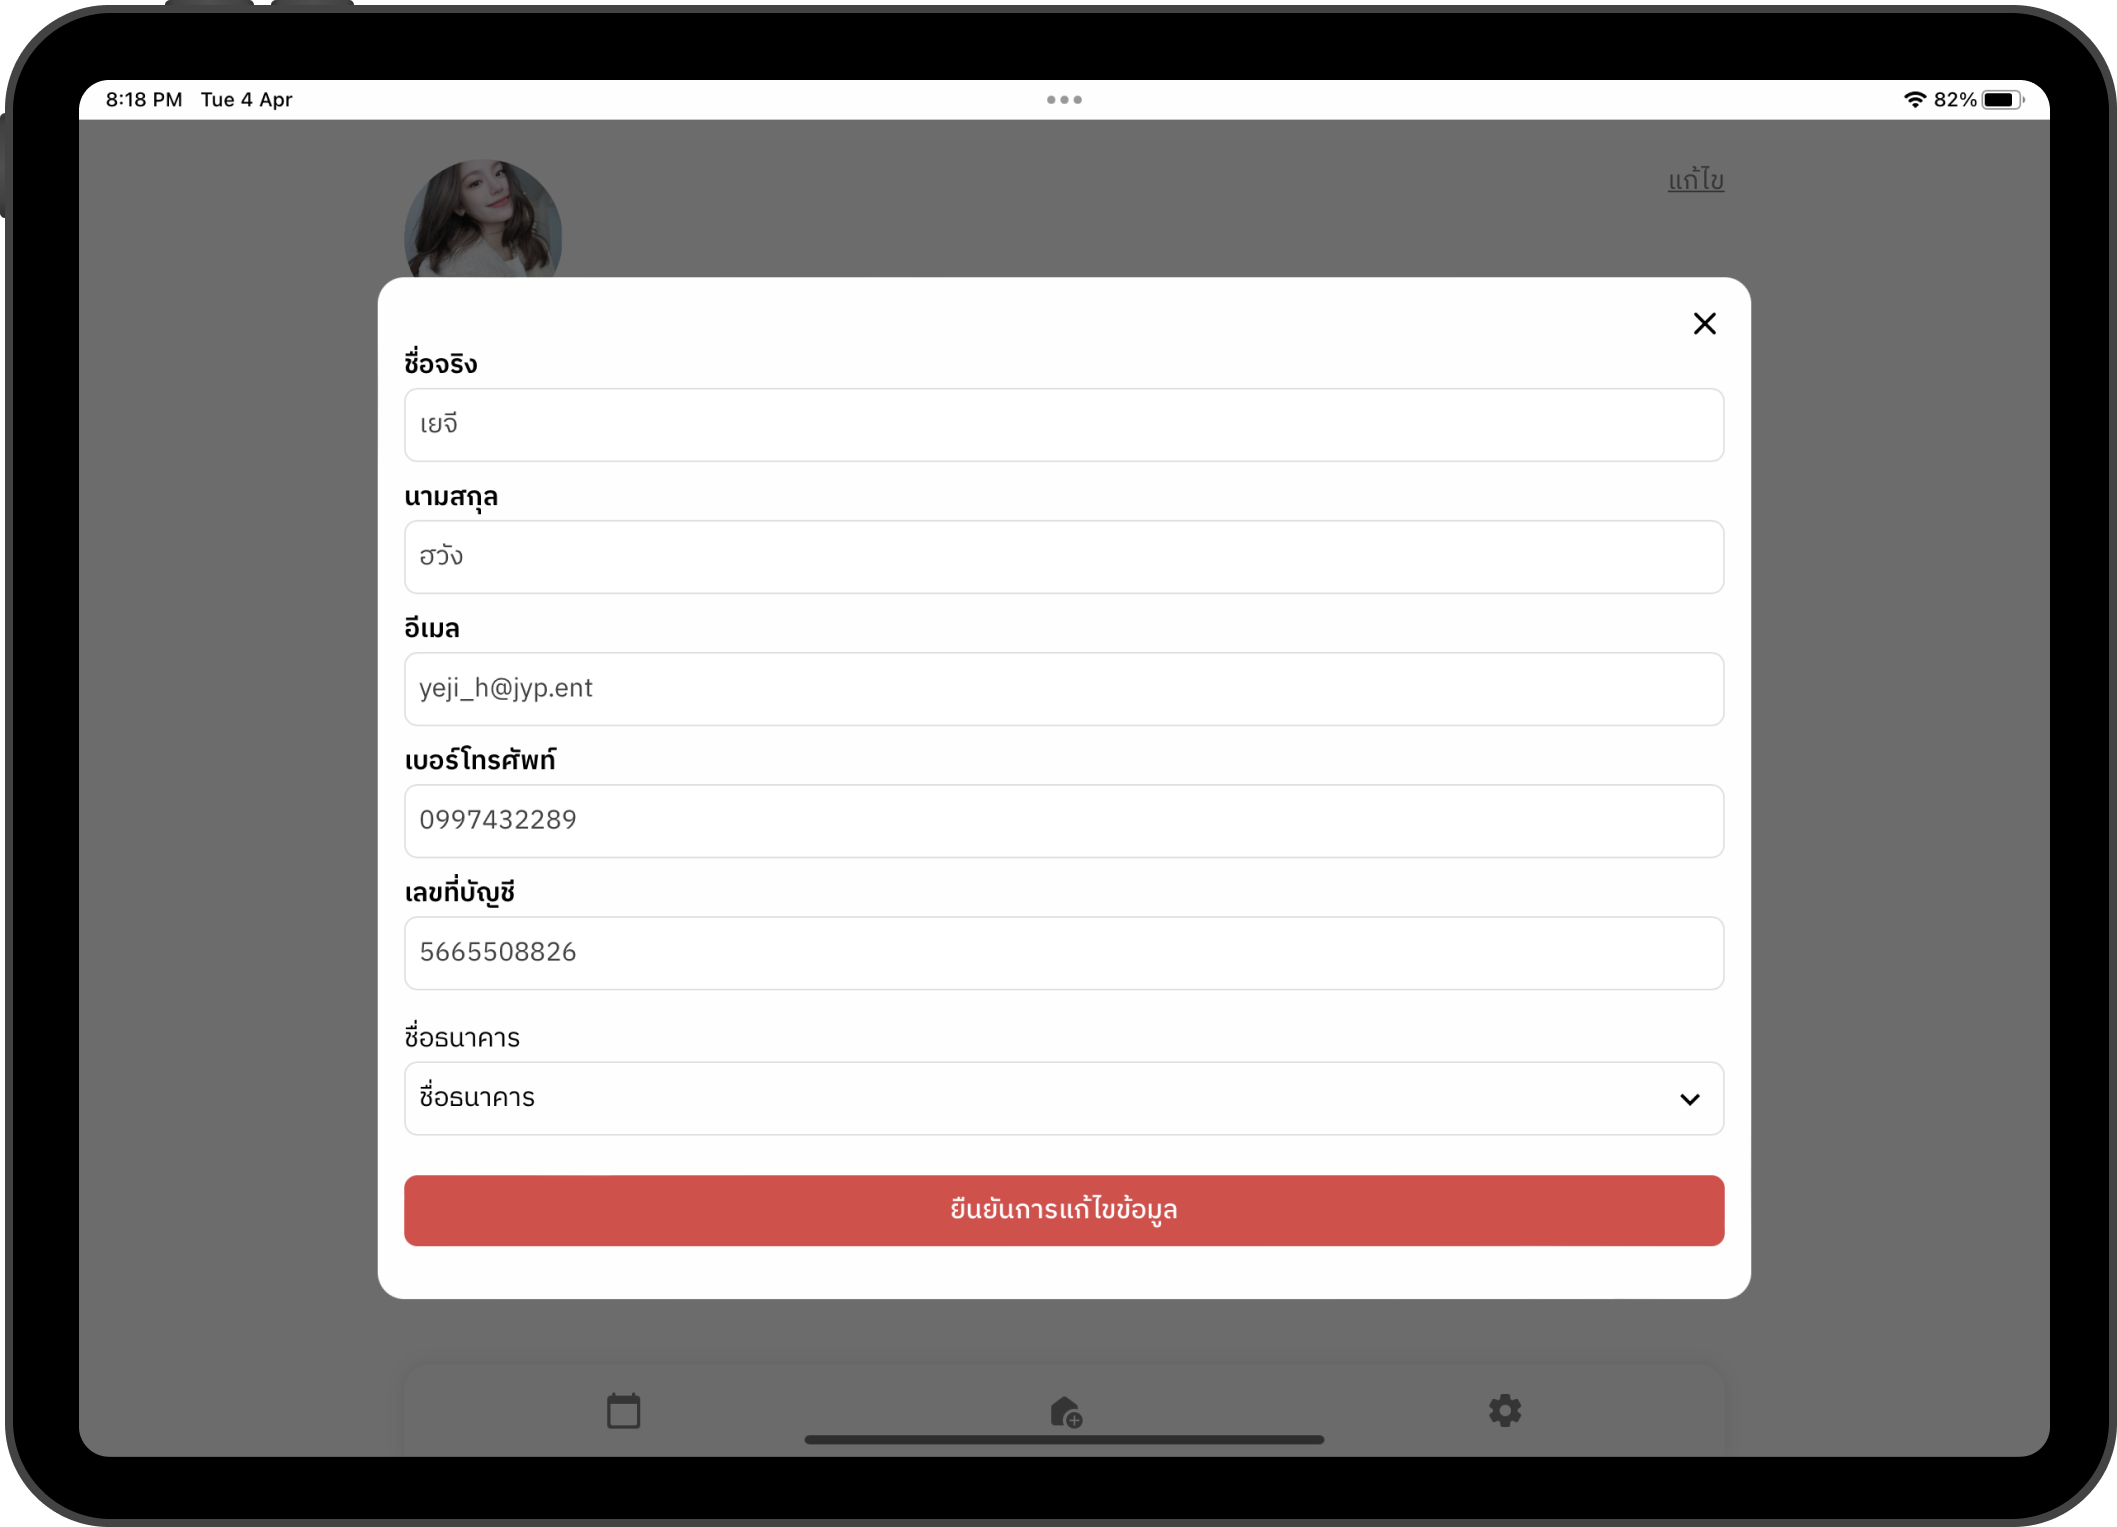
\includegraphics[width=5.5in]{./image/Flowider_edit_account.png}
    \end{center}
    \caption[Flowider edit account]{หน้าแก้ไขข้อมูลส่วนตัวของผู้ให้บริการ}
    \label{fig:Flowider_edit_account}
\end{figure}
\begin{figure}[ht]
    \begin{center}
    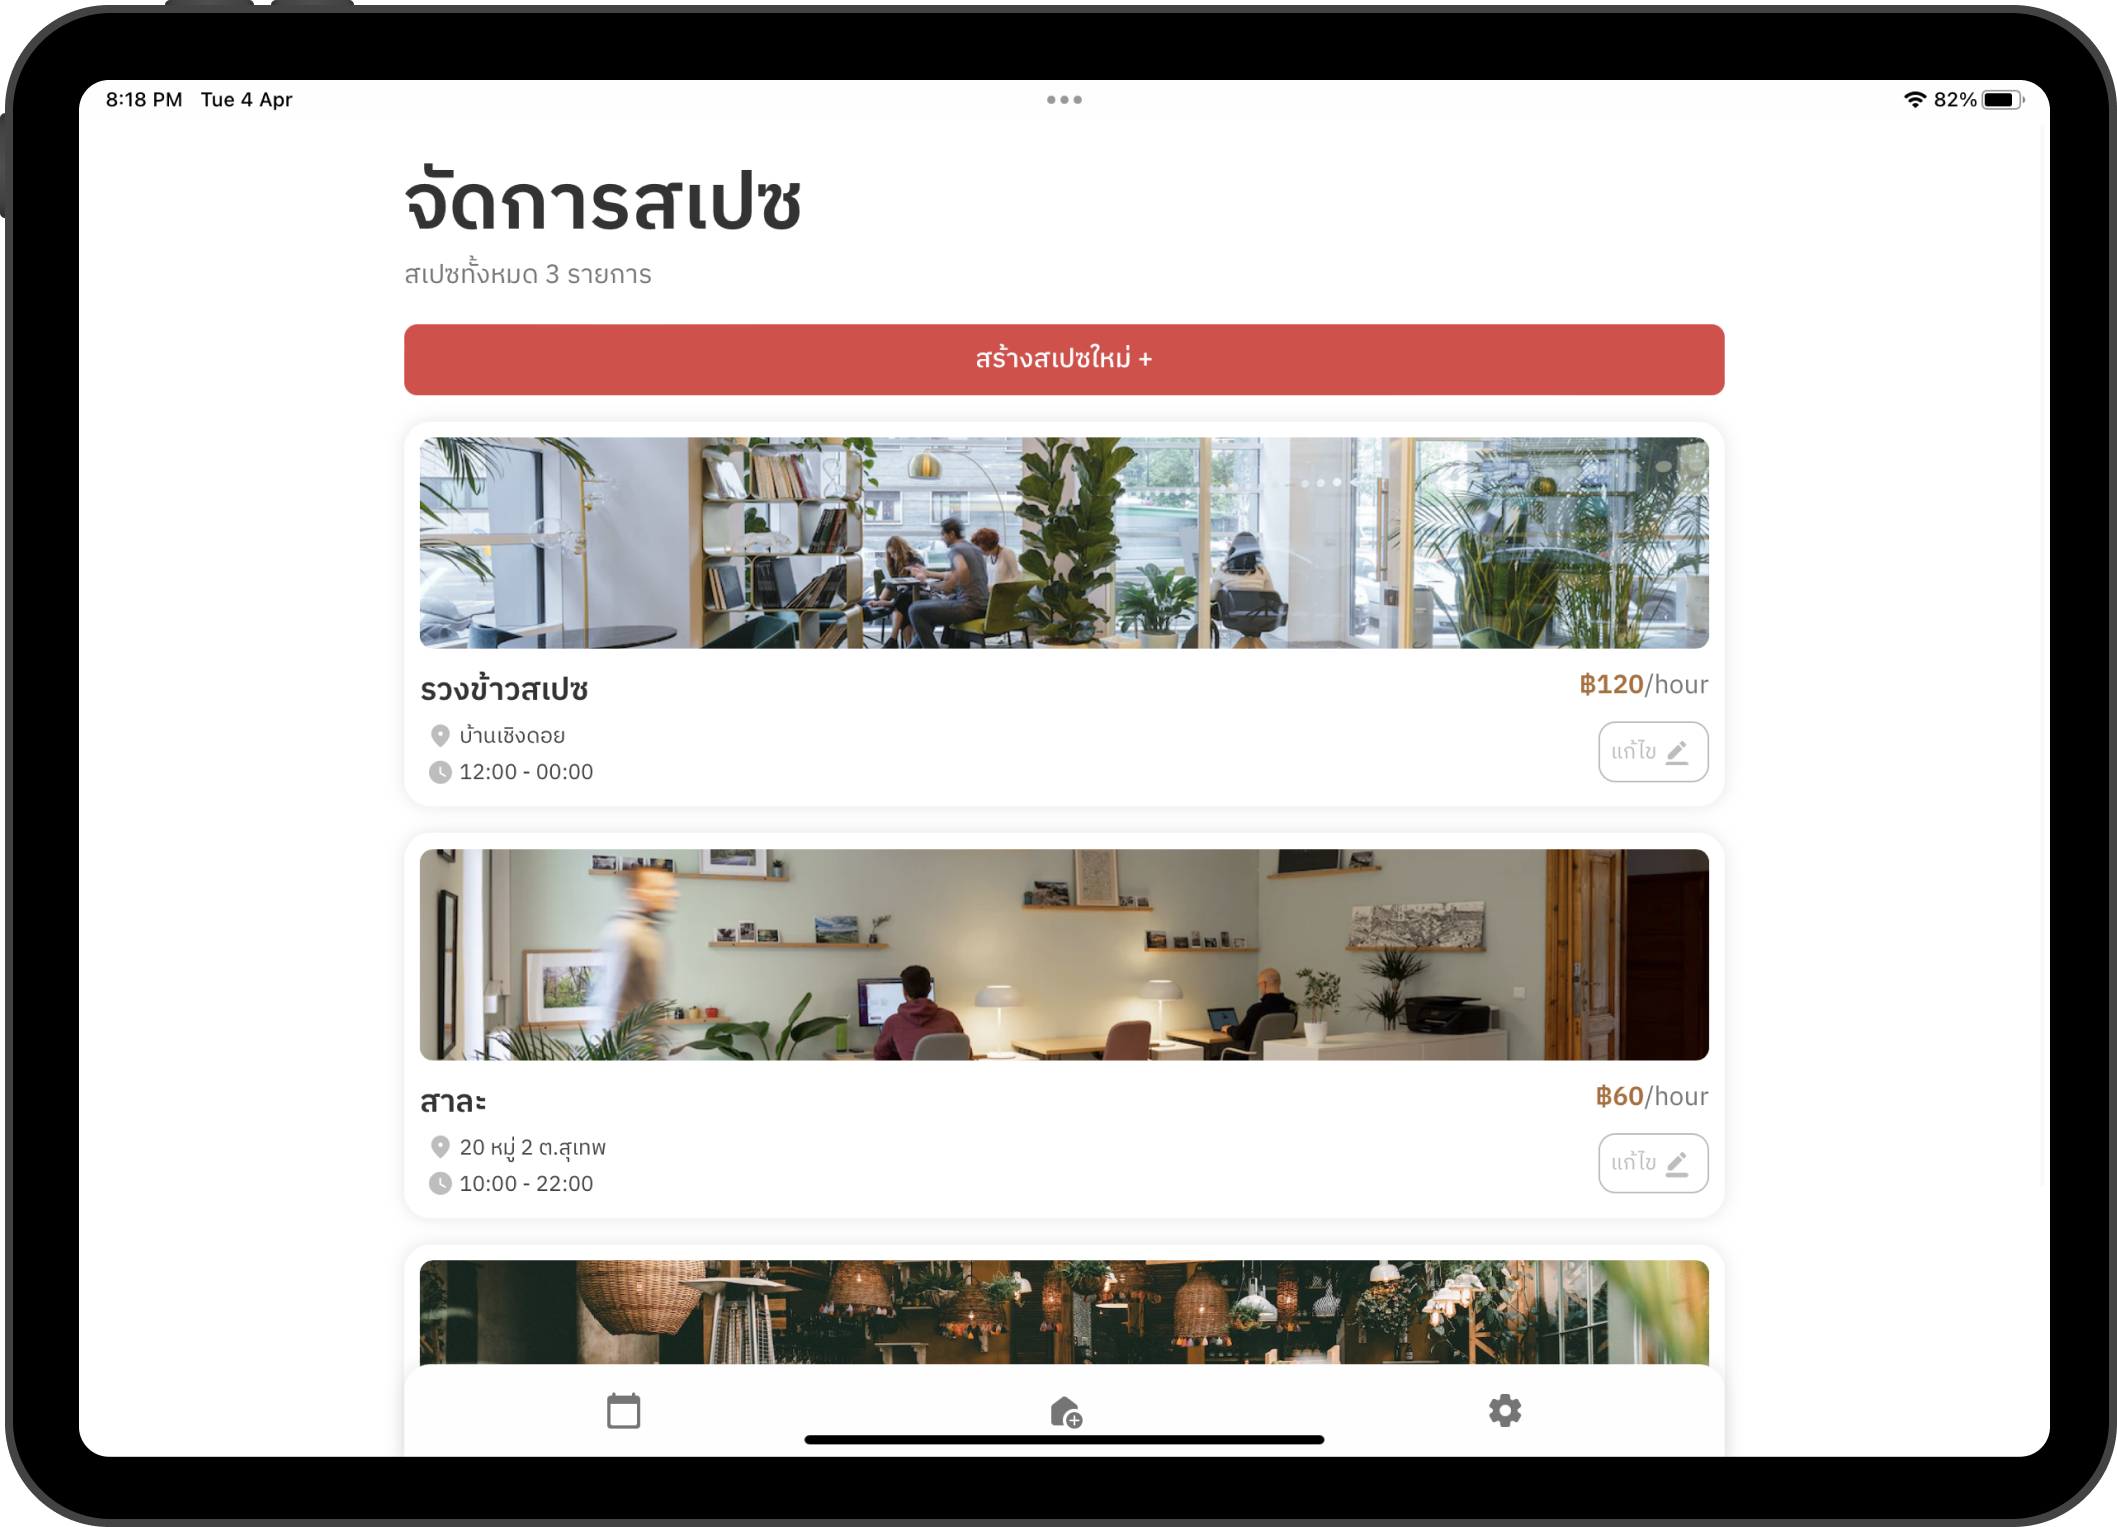
\includegraphics[width=5.5in]{./image/Flowider_space_mgmt.png}
    \end{center}
    \caption[Flowider space management]{หน้าจัดการสเปซ}
    \label{fig:Flowider_space_mgmt}
\end{figure}
\begin{figure}[ht]
    \begin{center}
    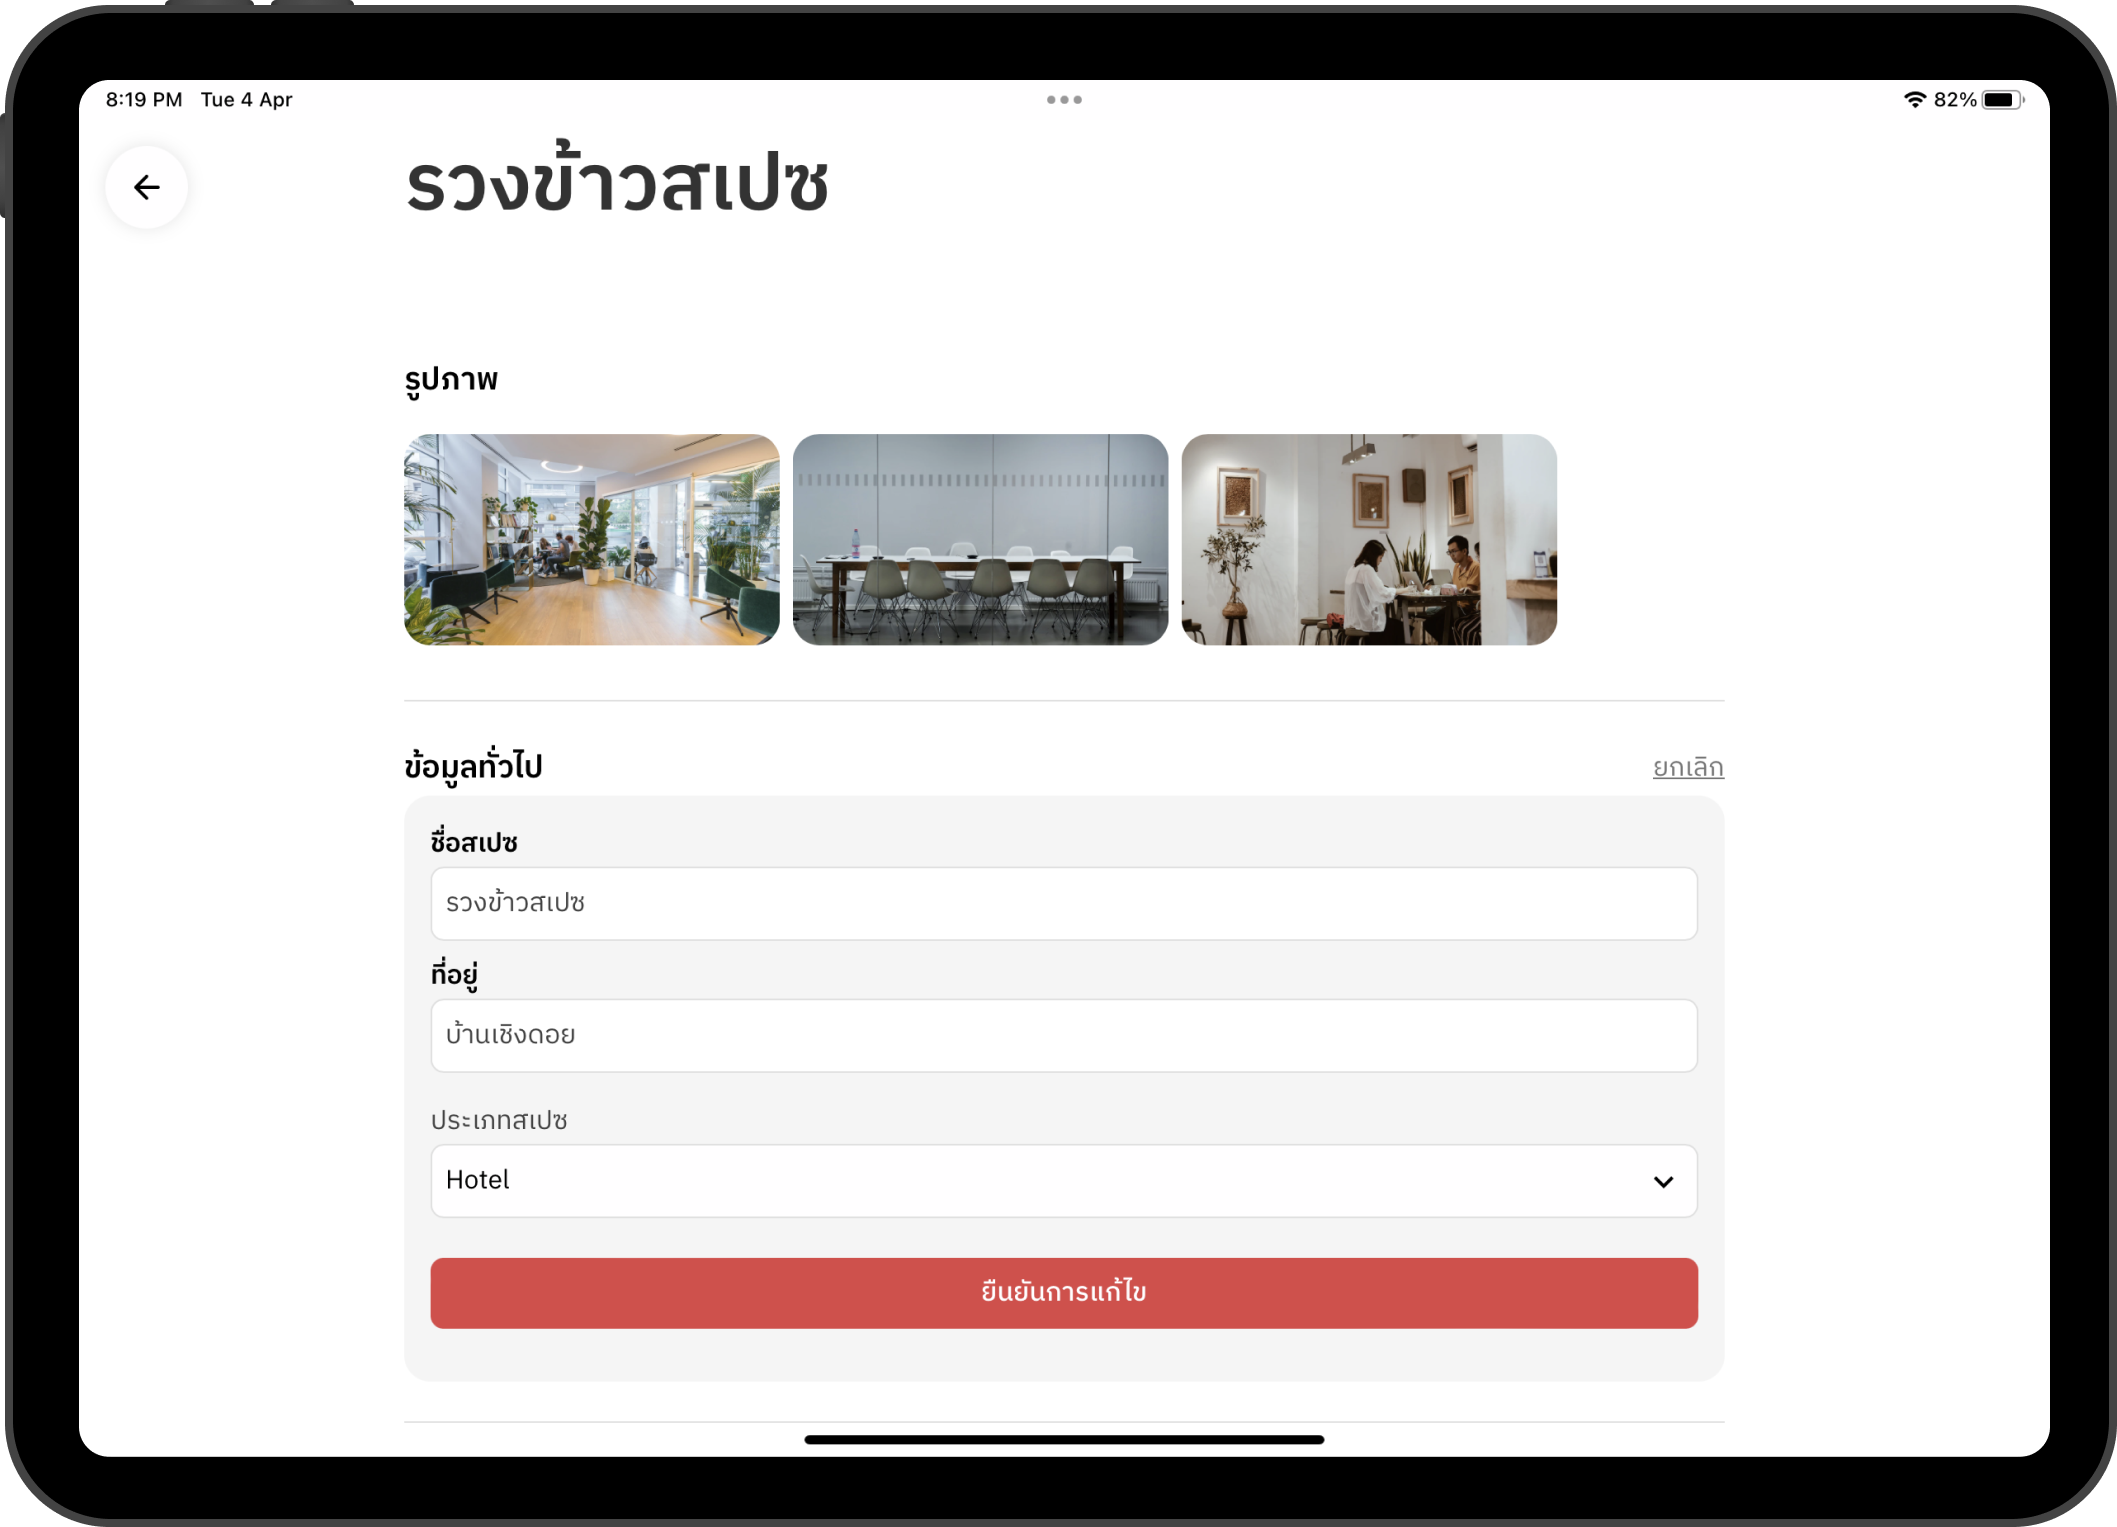
\includegraphics[width=5.5in]{./image/Flowider_space_edit_1.png}
    \end{center}
    \caption[Flowider space edit 1]{หน้าแก้ไขข้อมูลของสเปซ}
    \label{fig:Flowider_space_edit_1}
\end{figure}
\begin{figure}[ht]
    \begin{center}
    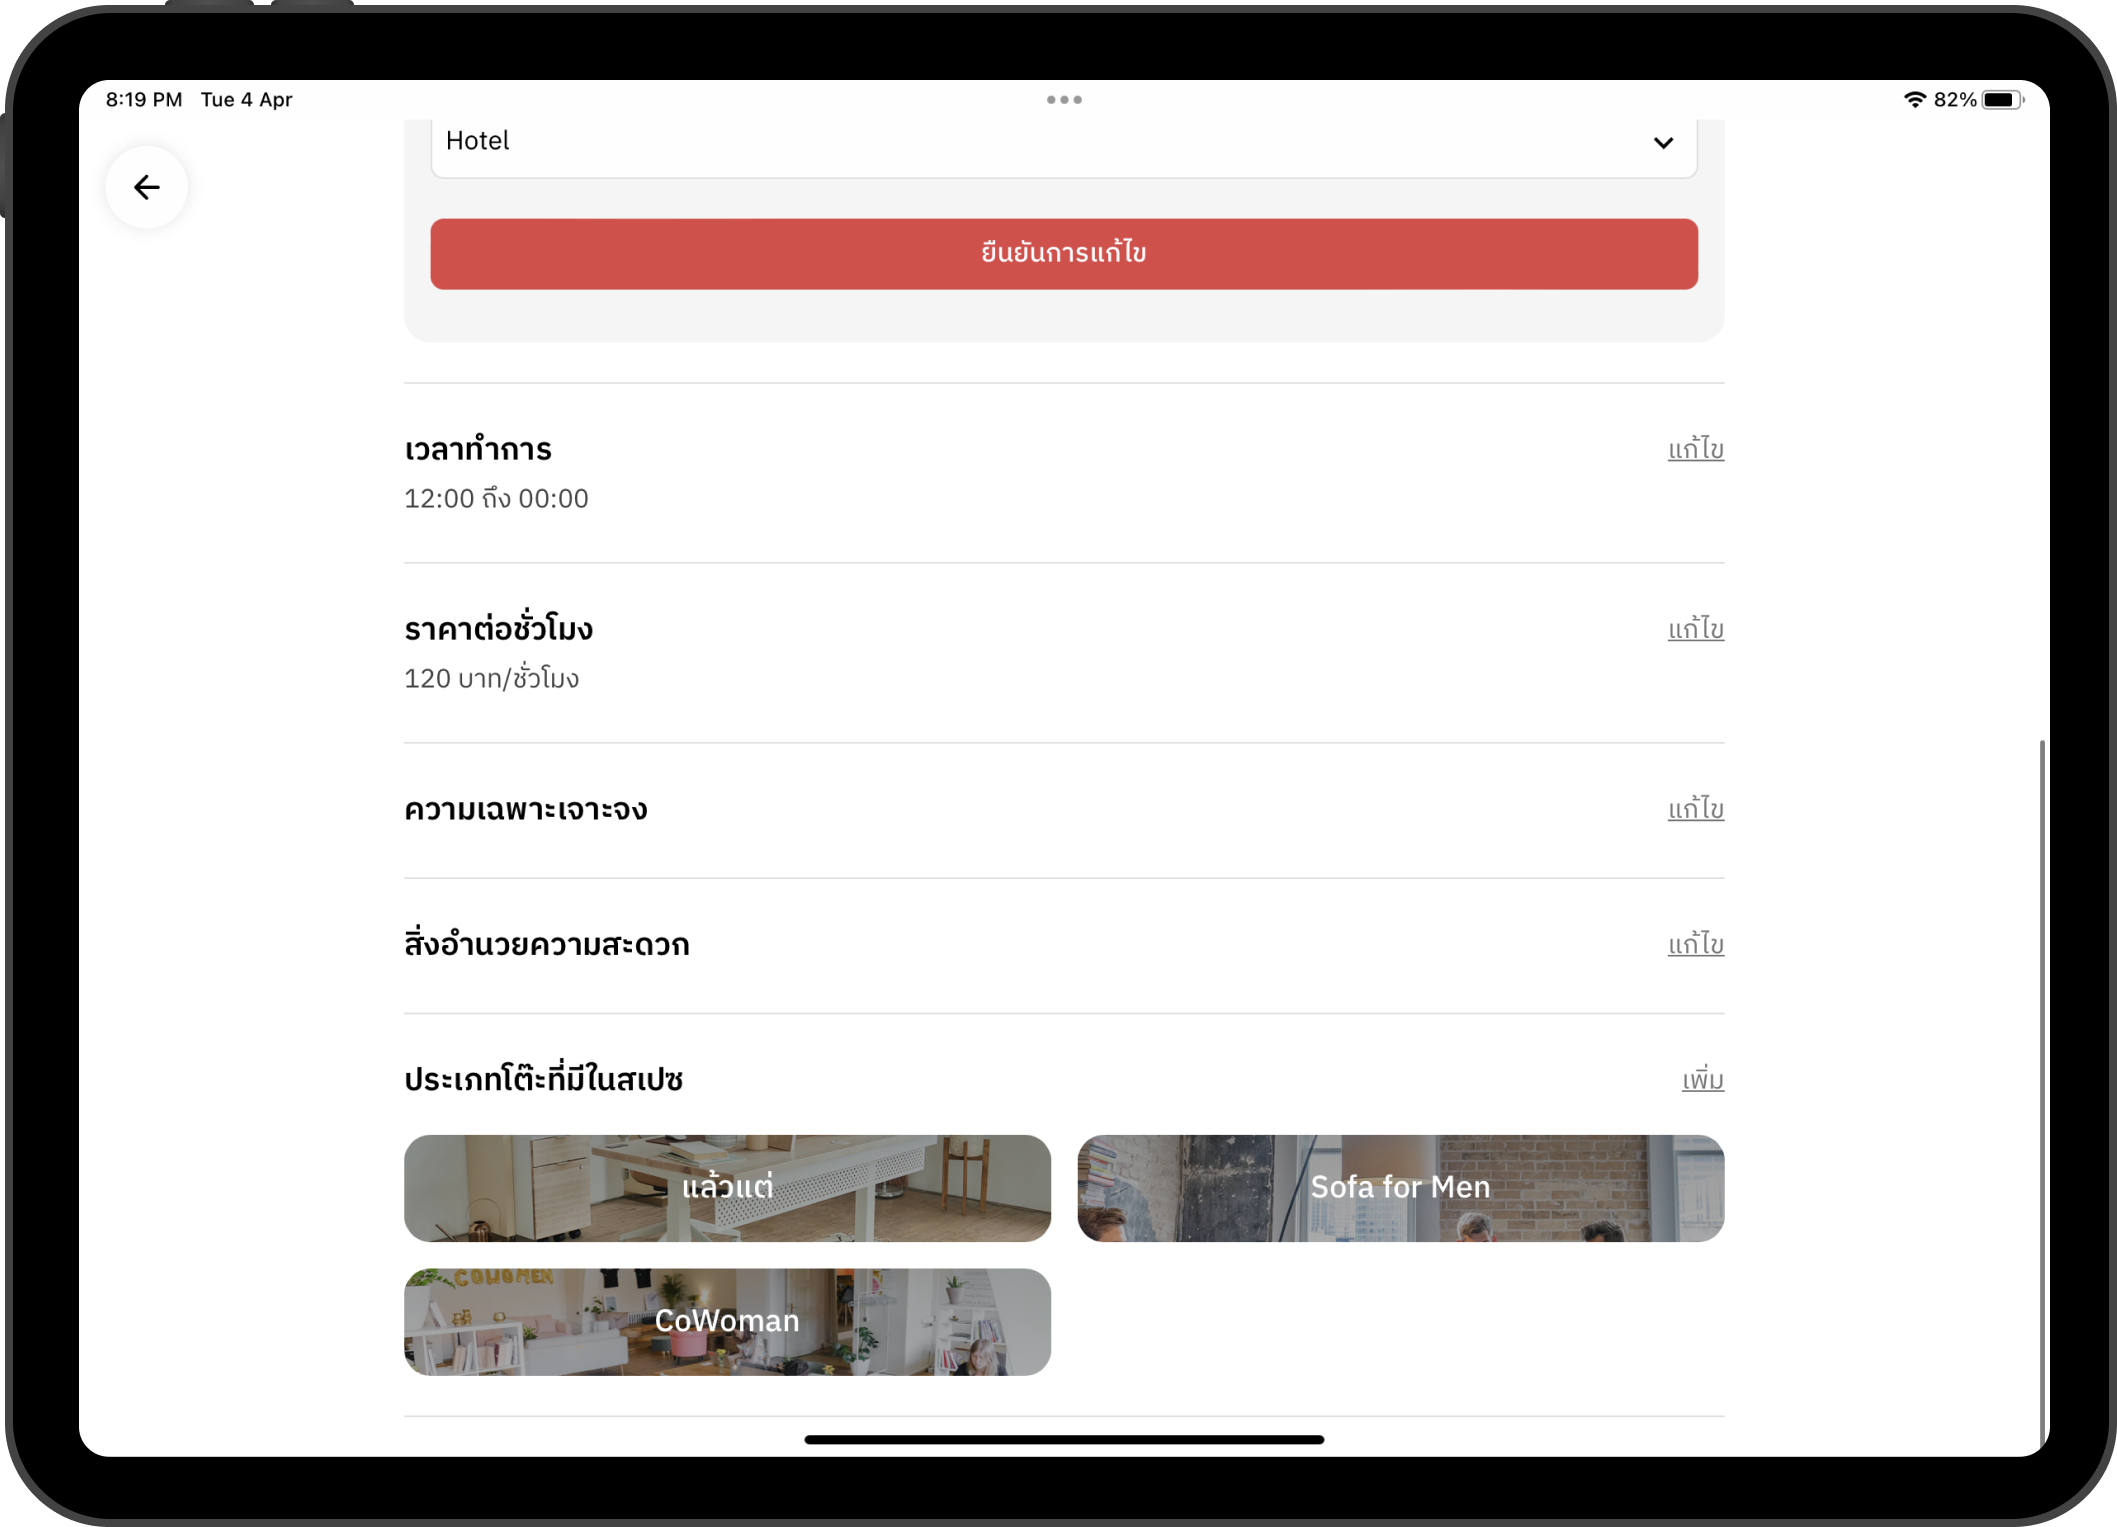
\includegraphics[width=5.5in]{./image/Flowider_space_edit_2.png}
    \end{center}
    \caption[Flowider space edit 2]{หน้าแก้ไขข้อมูลของสเปซ (ต่อ)}
    \label{fig:Flowider_space_edit_2}
\end{figure}
\begin{figure}[ht]
    \begin{center}
    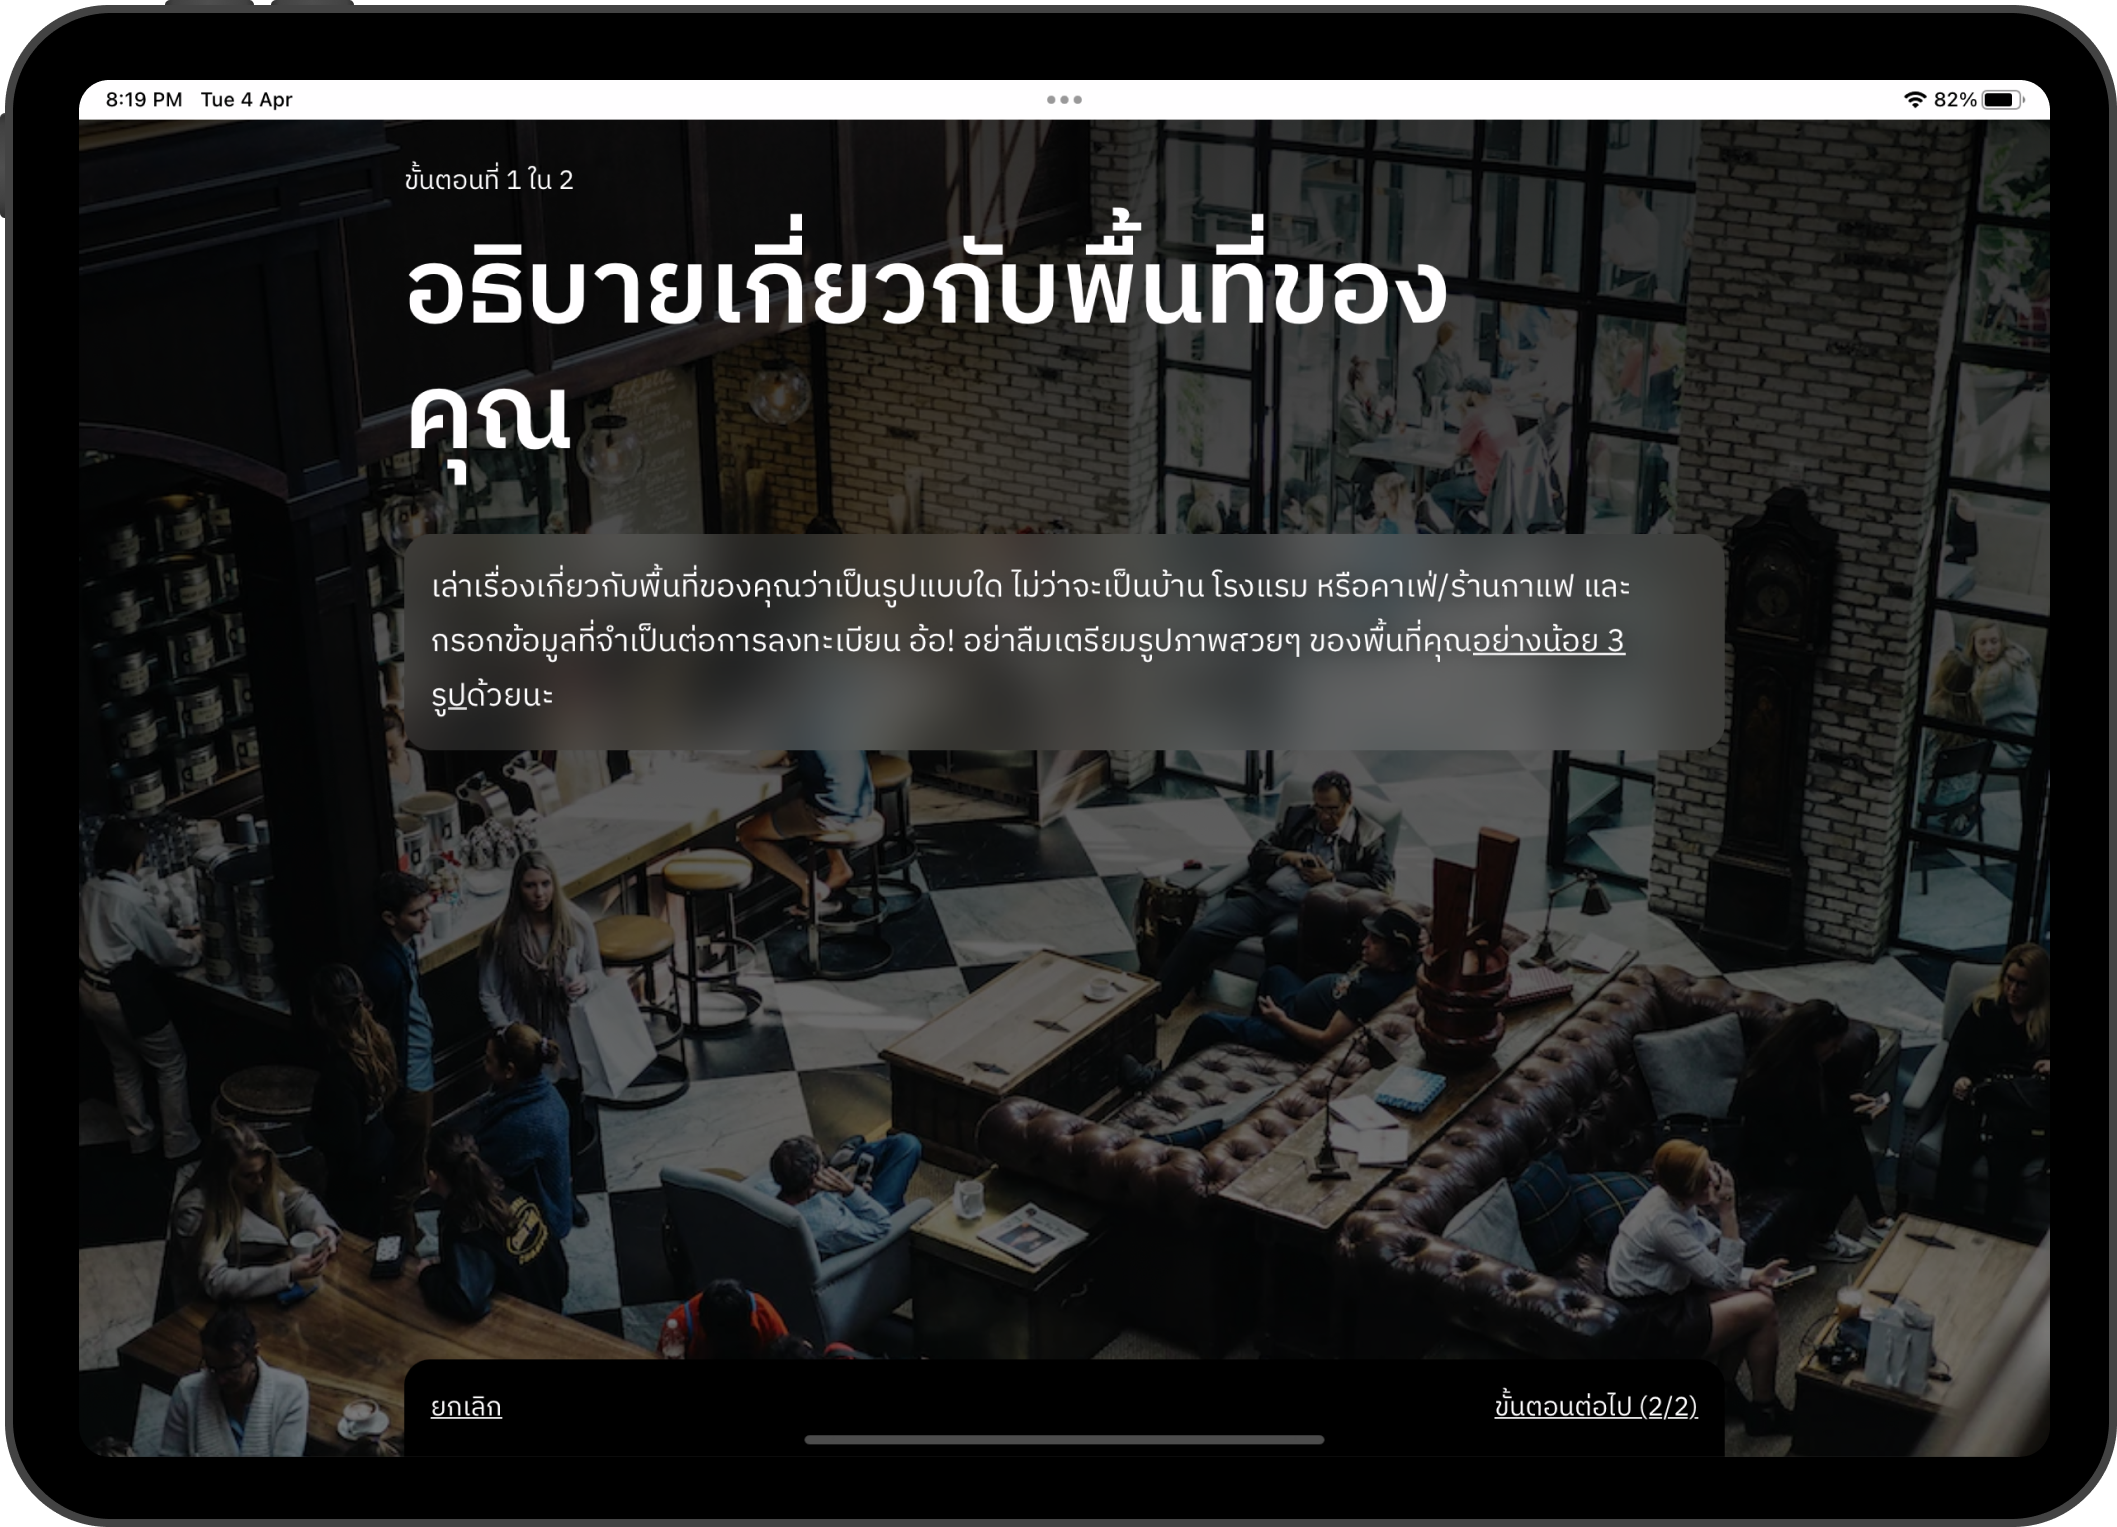
\includegraphics[width=5.5in]{./image/Flowider_onboarding_1.png}
    \end{center}
    \caption[Flowider onboarding 1]{หน้าเตรียมข้อมูลของสเปซก่อนทำการลงทะเบียน}
    \label{fig:Flowider_onboarding_1}
\end{figure}
\begin{figure}[ht]
    \begin{center}
    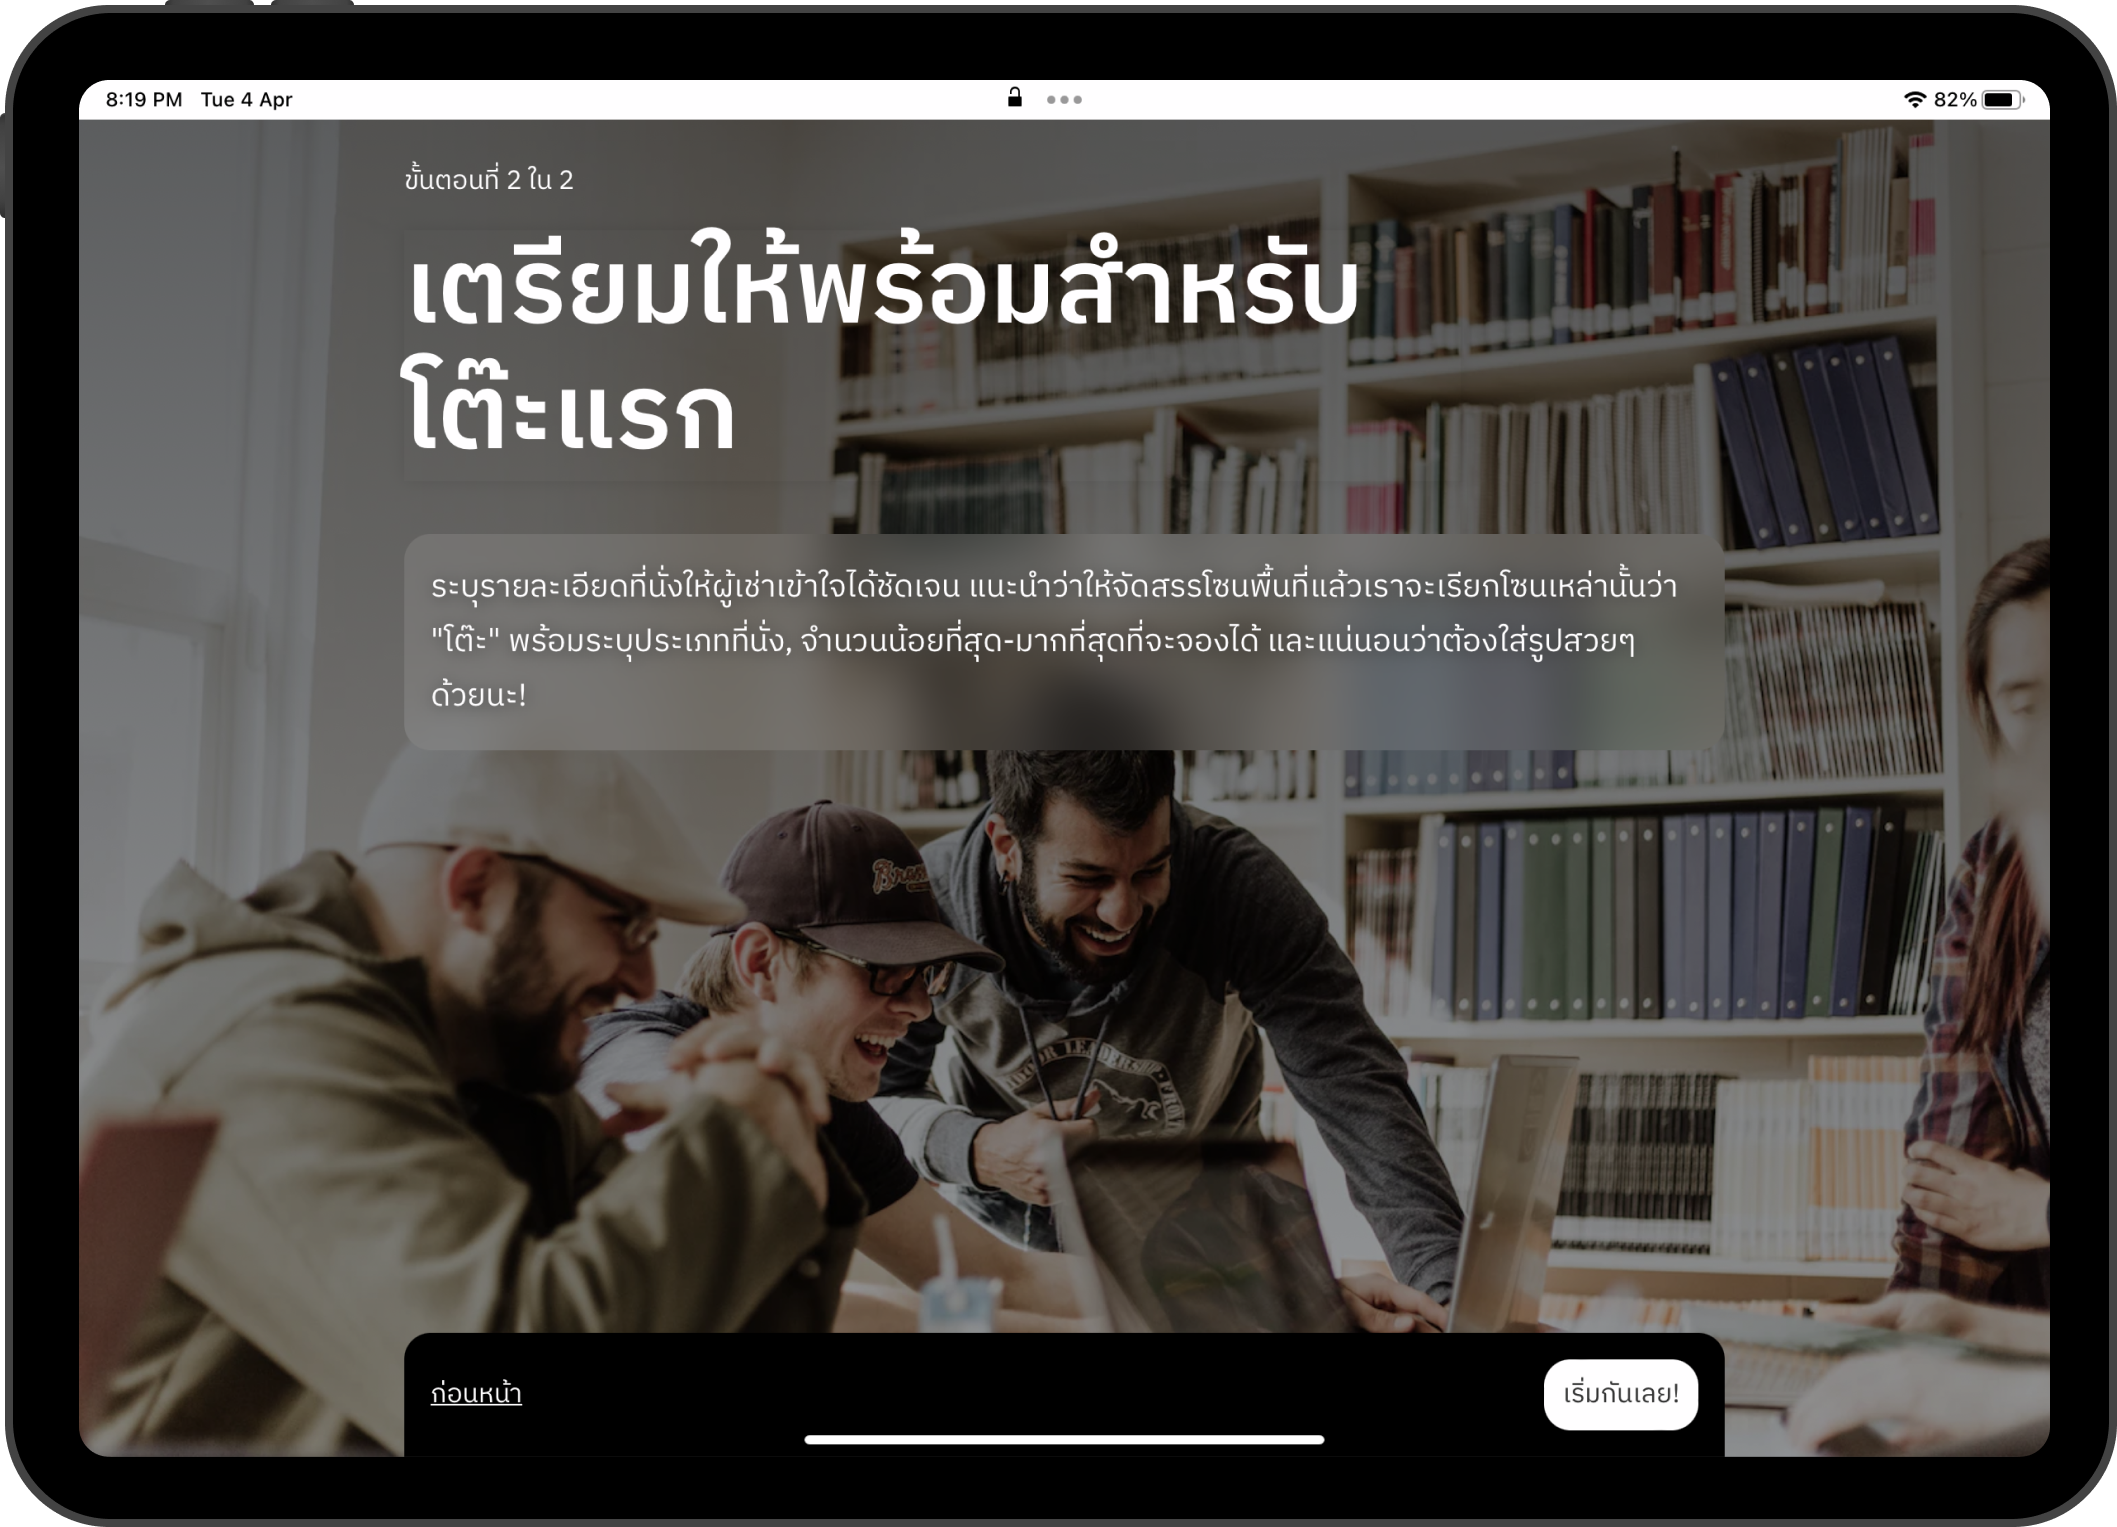
\includegraphics[width=5.5in]{./image/Flowider_onboarding_2.png}
    \end{center}
    \caption[Flowider onboarding 2]{หน้าเตรียมข้อมูลของโต๊ะก่อนทำการลงทะเบียน}
    \label{fig:Flowider_onboarding_2}
\end{figure}
\begin{figure}[ht]
    \begin{center}
    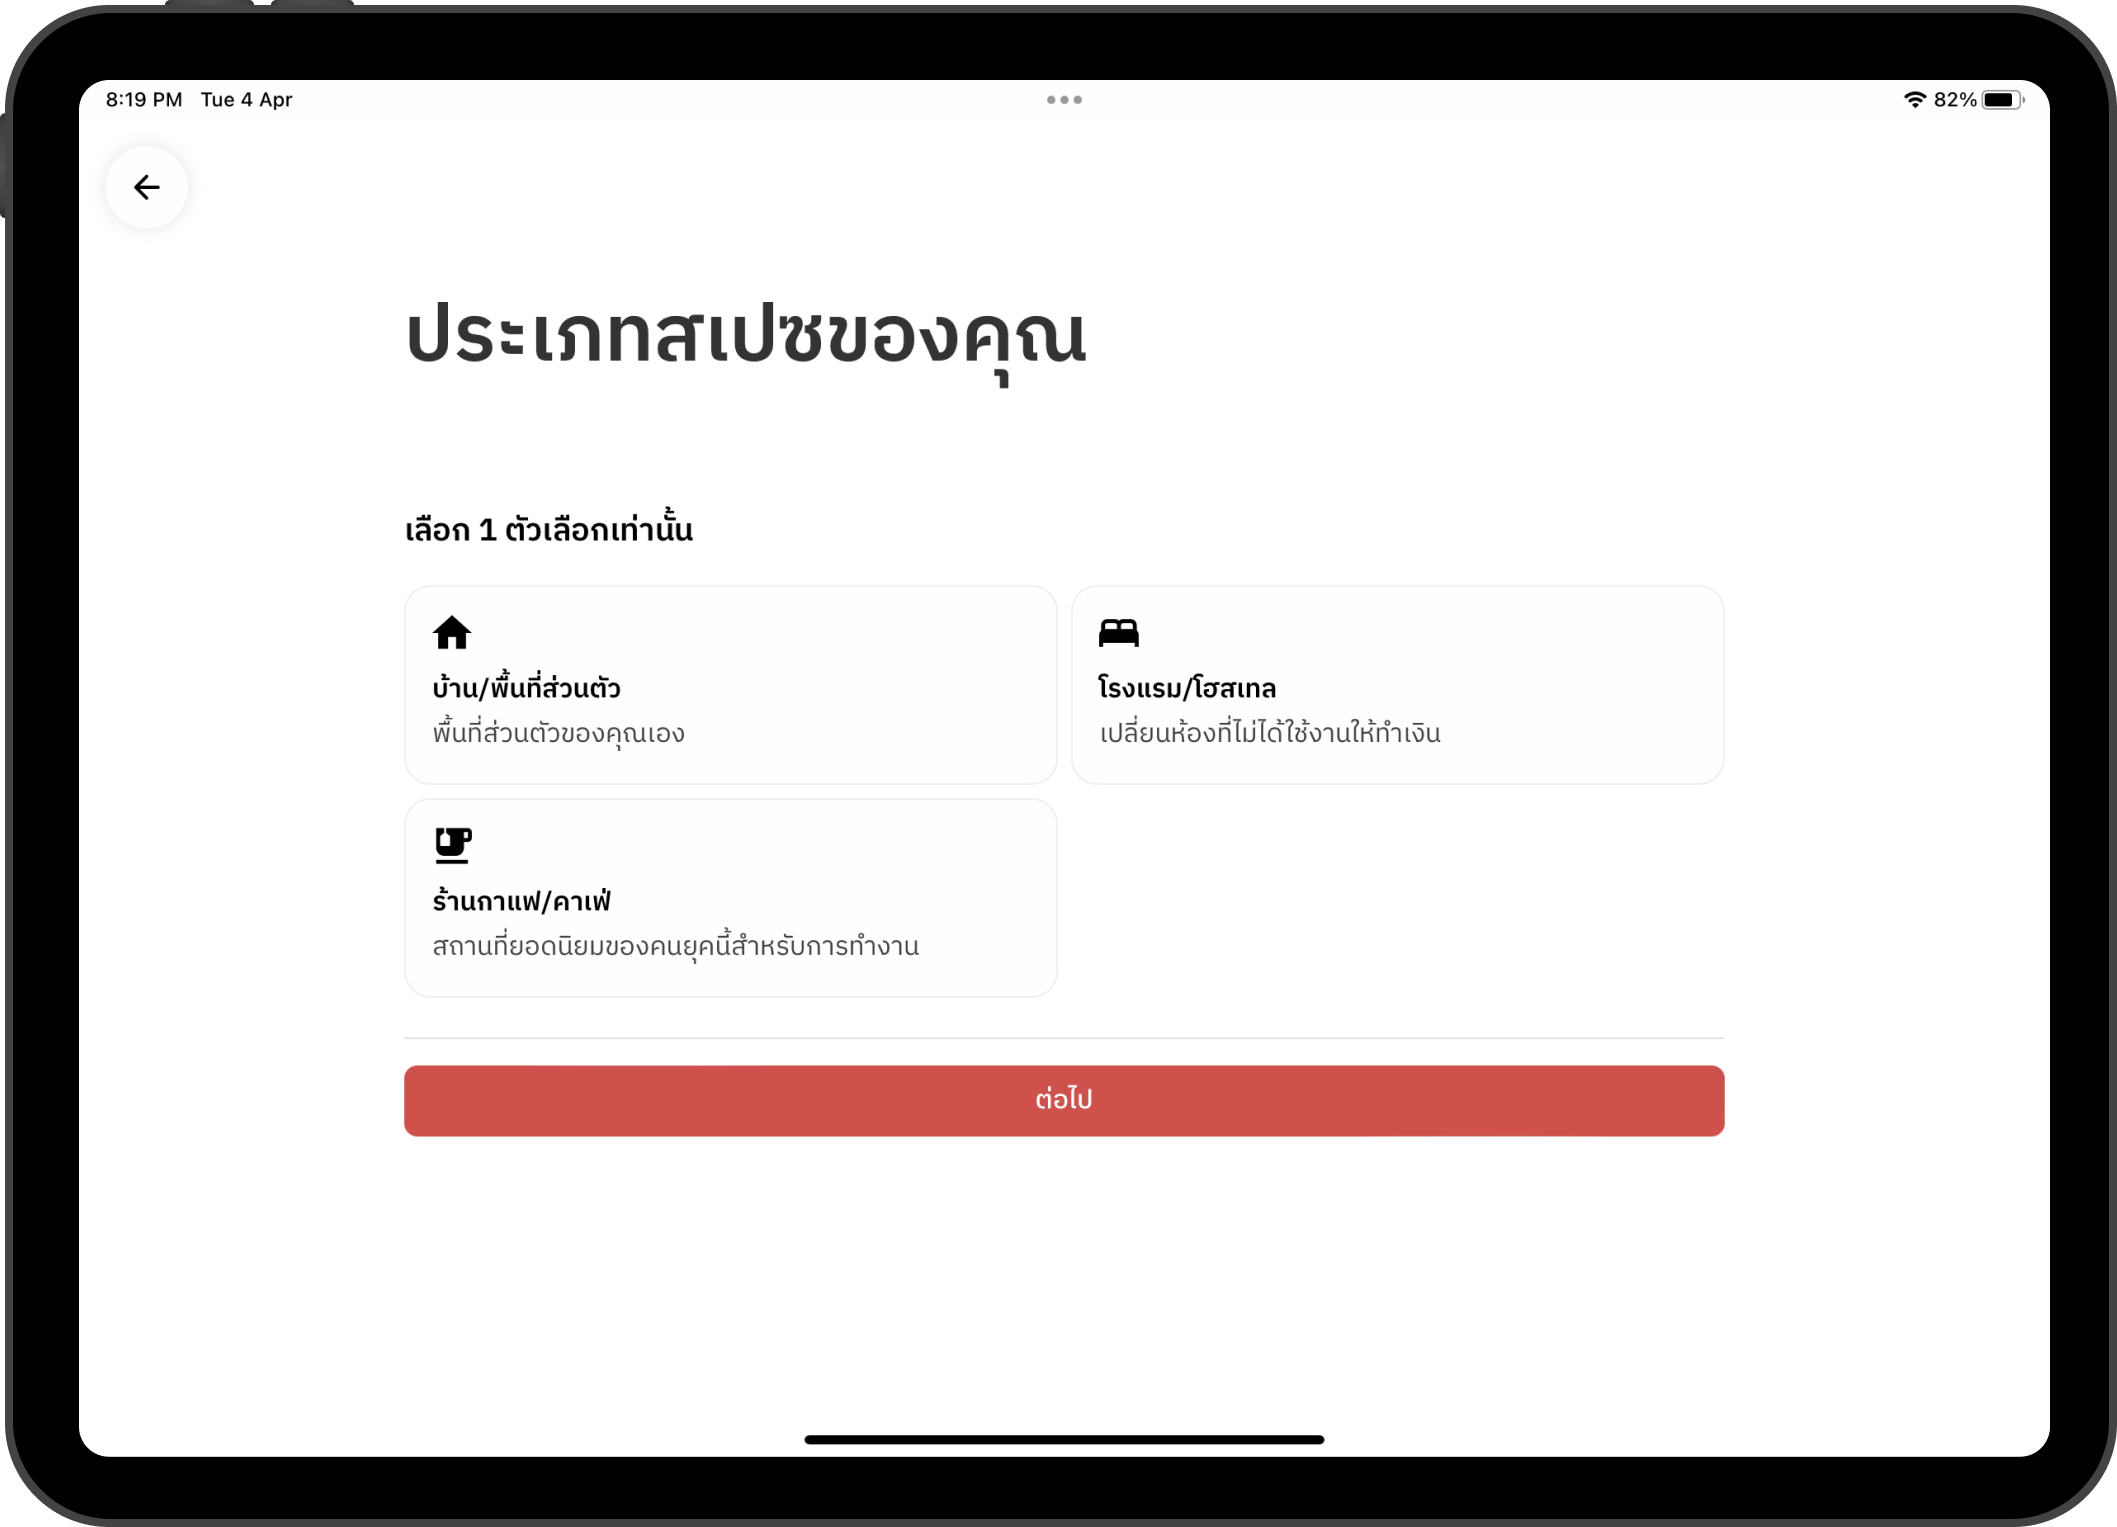
\includegraphics[width=5.5in]{./image/Flowider_place_category.png}
    \end{center}
    \caption[Flowider place category]{หน้าระบุประเภทของสเปซ}
    \label{fig:Flowider_place_category}
\end{figure}
\begin{figure}[ht]
    \begin{center}
    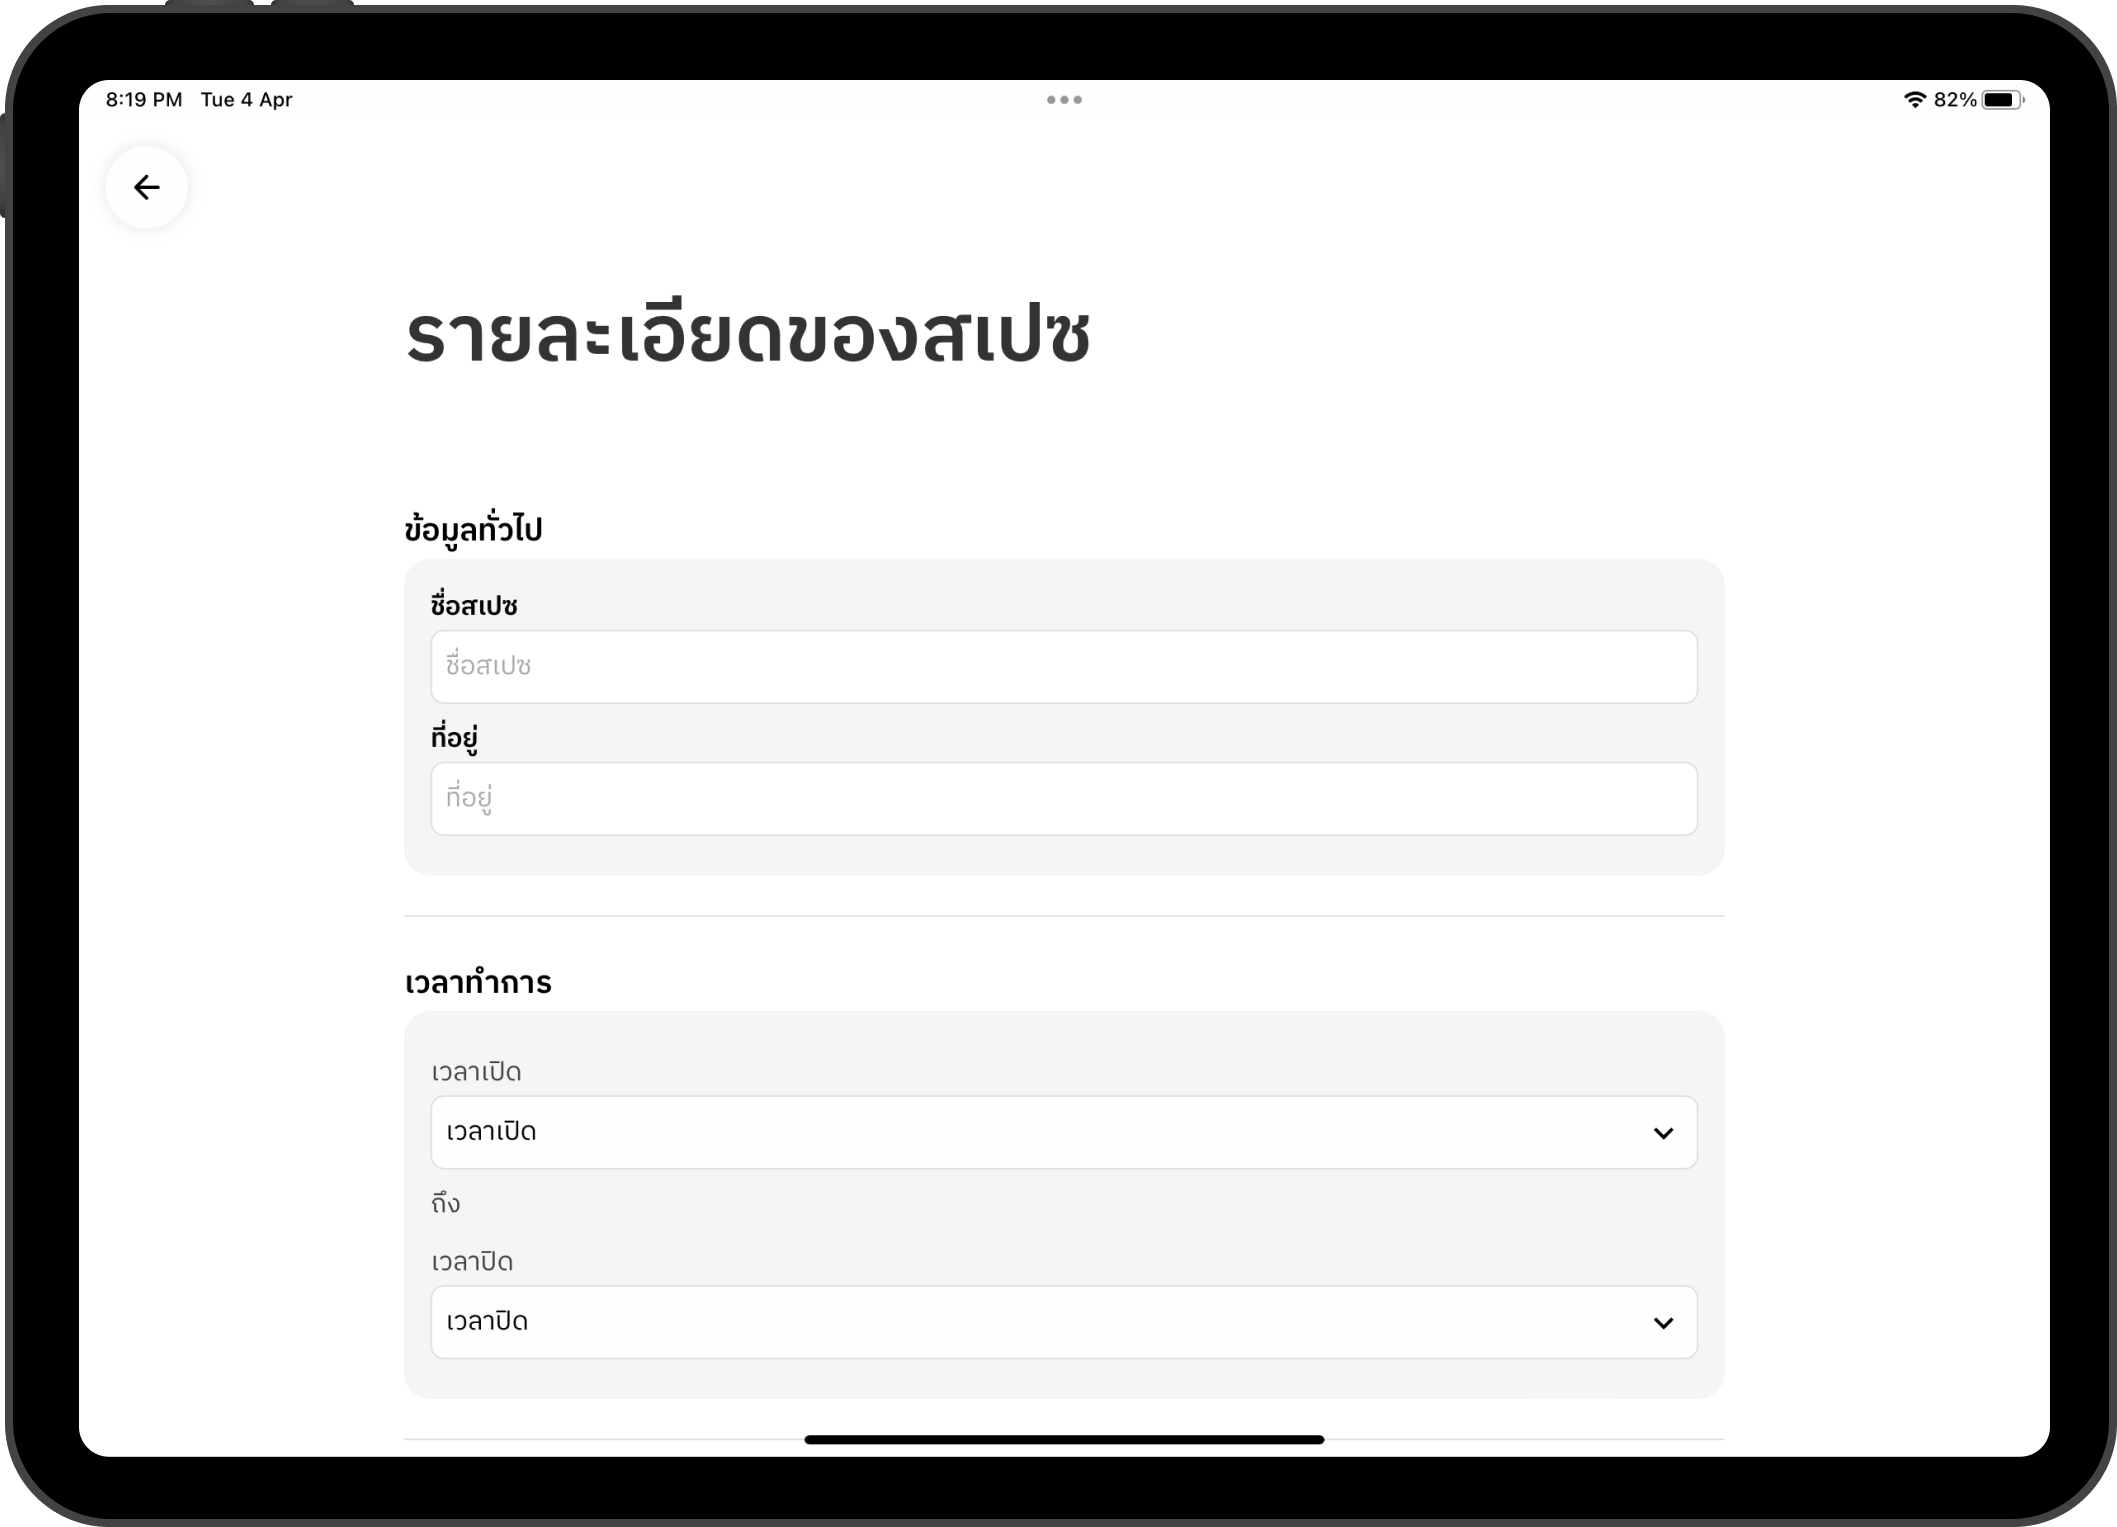
\includegraphics[width=5.5in]{./image/Flowider_place_info_1.png}
    \end{center}
    \caption[Flowider place info 1]{หน้าระบุรายละเอียดของสเปซ}
    \label{fig:Flowider_place_info_1}
\end{figure}
\begin{figure}[ht]
    \begin{center}
    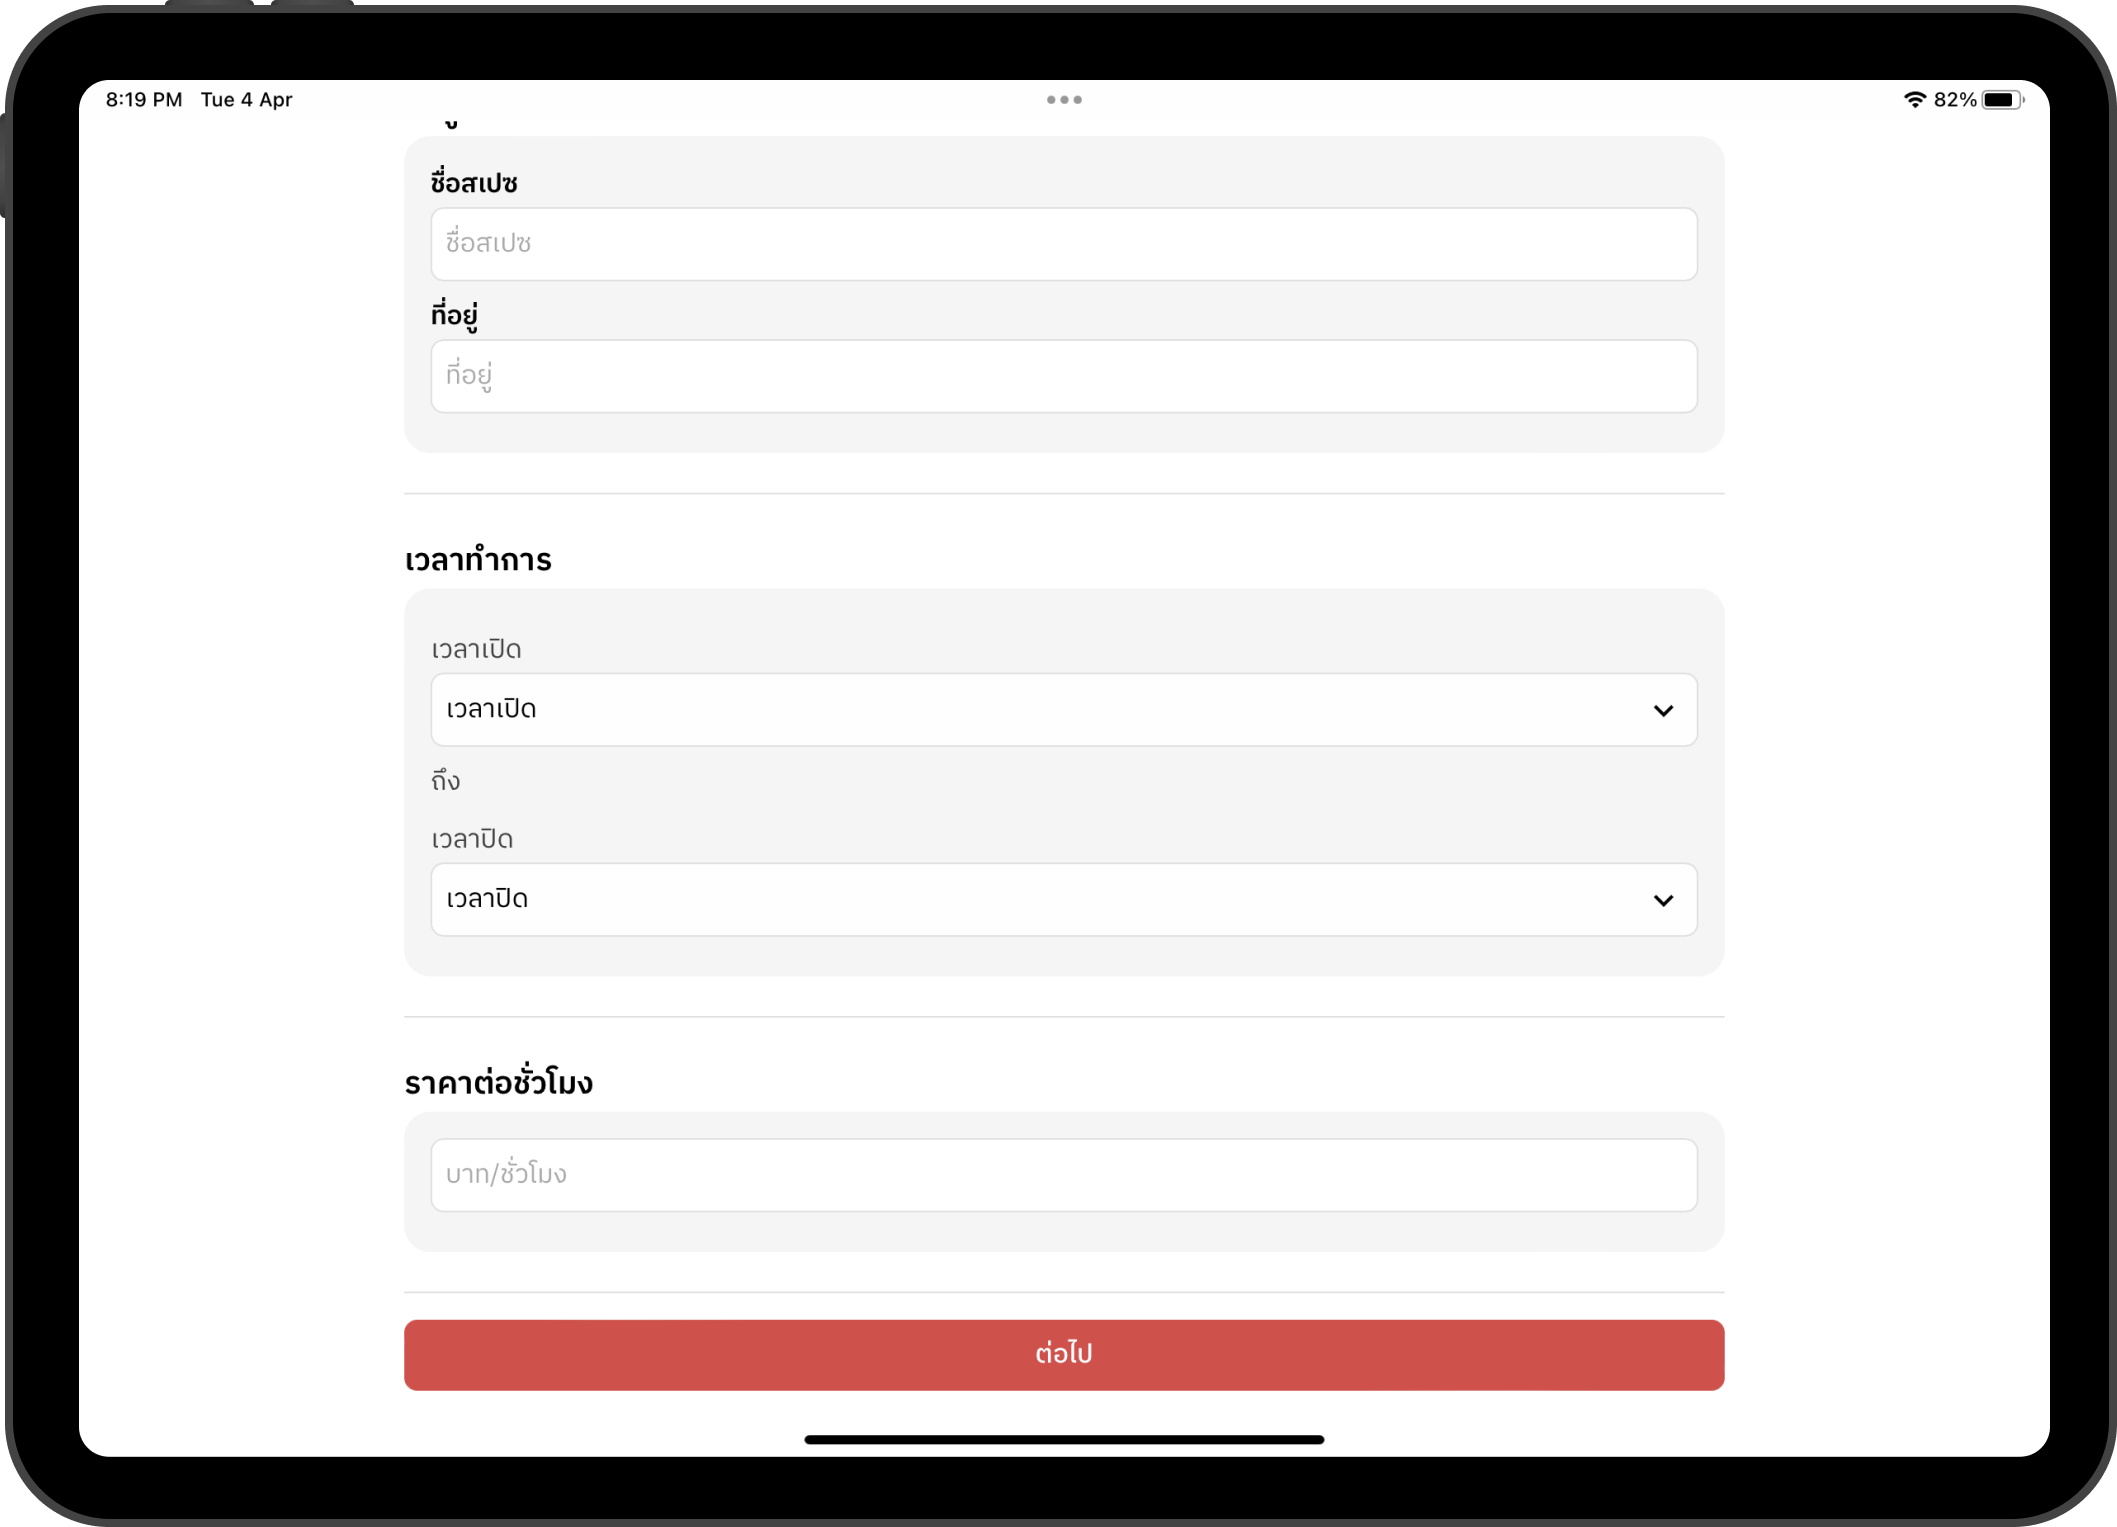
\includegraphics[width=5.5in]{./image/Flowider_place_info_2.png}
    \end{center}
    \caption[Flowider place info 2]{หน้าระบุรายละเอียดของสเปซ (ต่อ)}
    \label{fig:Flowider_place_info_2}
\end{figure}
\begin{figure}[ht]
    \begin{center}
    \includegraphics[width=5.5in]{./image/Flowider_place_Specification.png}
    \end{center}
    \caption[Flowider place Specification]{หน้าระบุความเฉาะเจาะจง}
    \label{fig:Flowider_place_Specification}
\end{figure}
\begin{figure}[ht]
    \begin{center}
    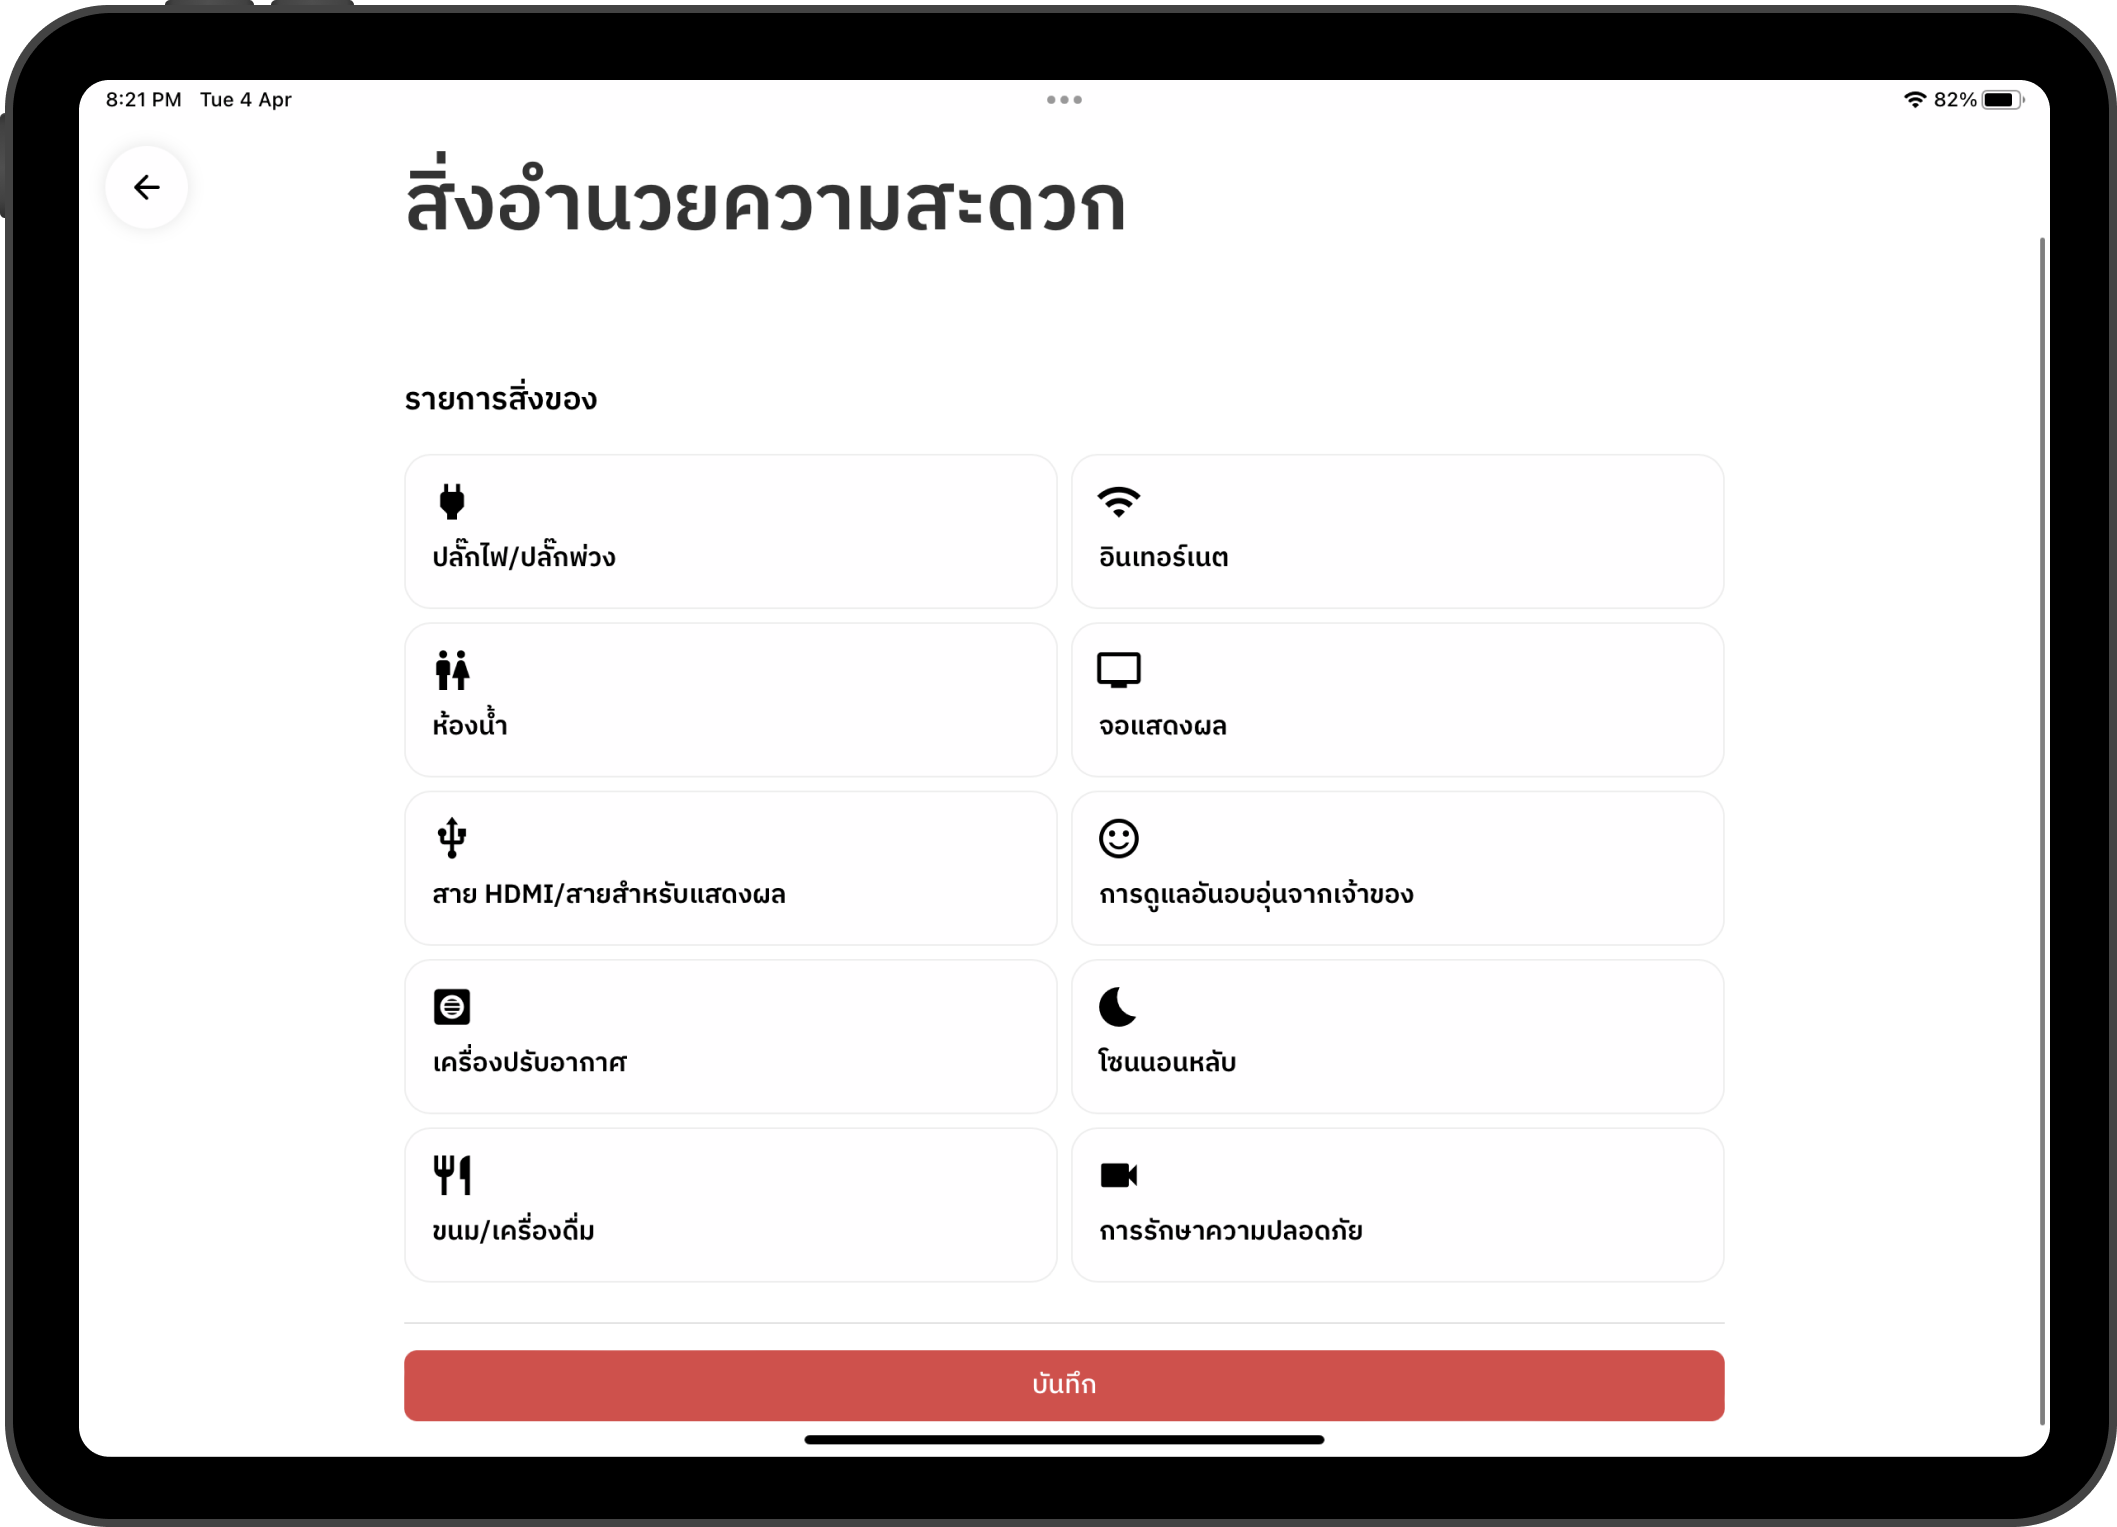
\includegraphics[width=5.5in]{./image/Flowider_place_amenity.png}
    \end{center}
    \caption[Flowider place amenity]{หน้าระบุสิ่งอำนวยความสะดวก}
    \label{fig:Flowider_place_amenity}
\end{figure}
\begin{figure}[ht]
    \begin{center}
    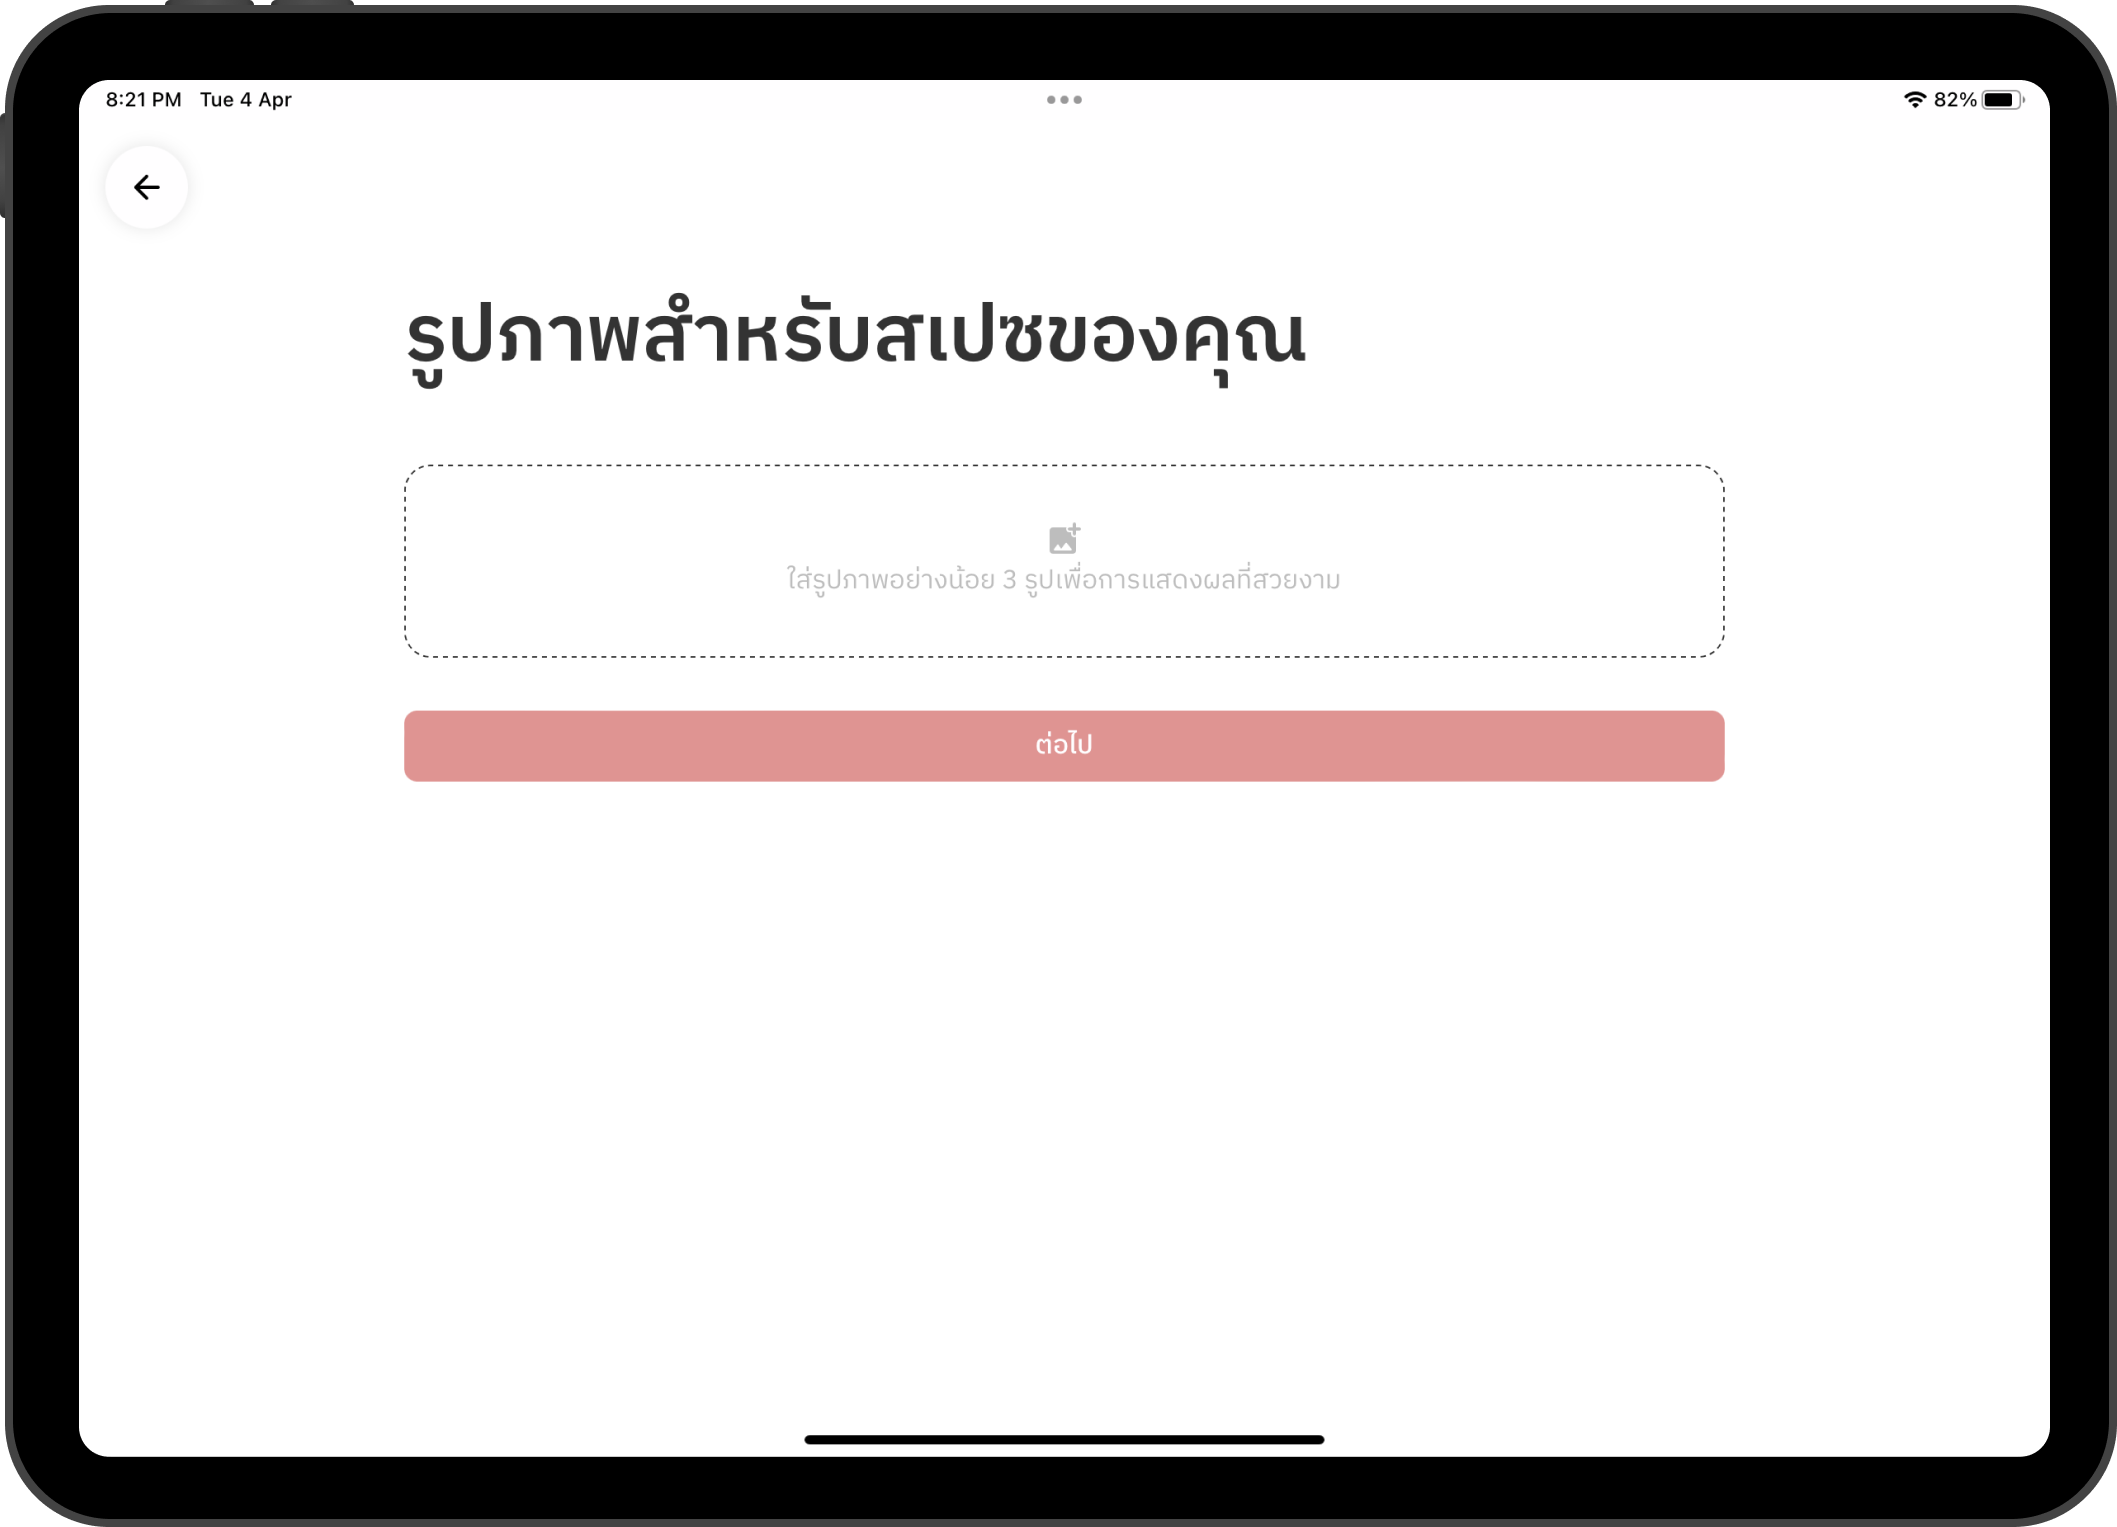
\includegraphics[width=5.5in]{./image/Flowider_place_img.png}
    \end{center}
    \caption[Flowider place image]{หน้าเพิ่มรูปภาพของสเปซ}
    \label{fig:Flowider_place_img}
\end{figure}
\begin{figure}[ht]
    \begin{center}
    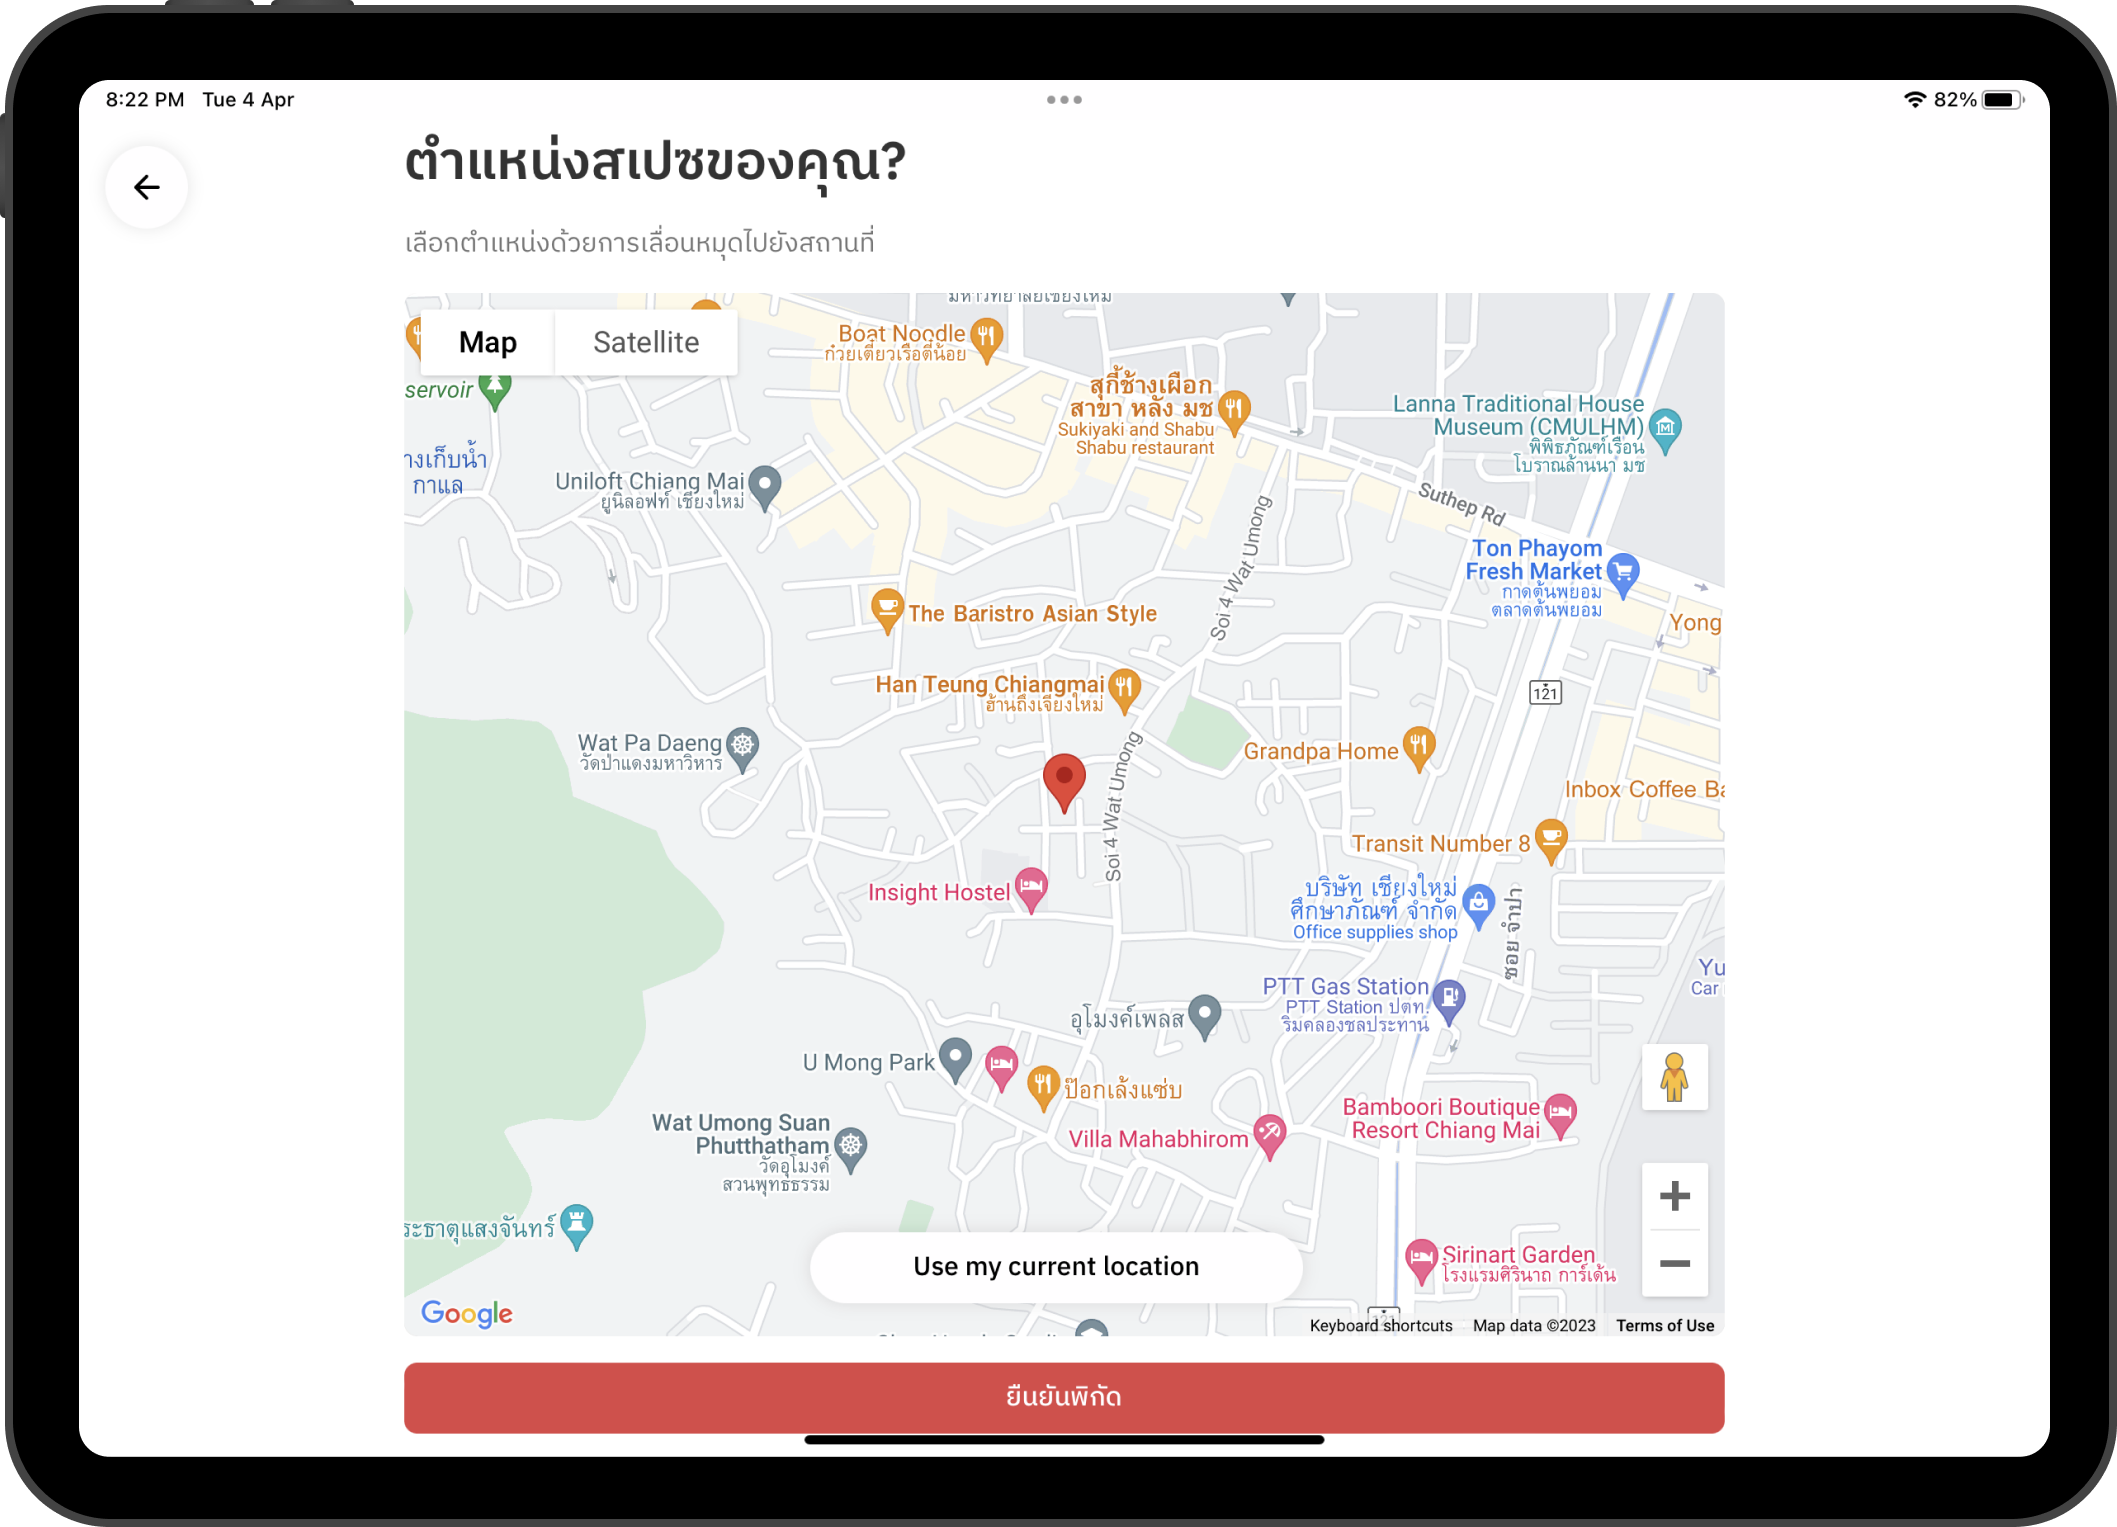
\includegraphics[width=5.5in]{./image/Flowider_place_location.png}
    \end{center}
    \caption[Flowider place location]{หน้าระบุตำแหน่งของสเปซ}
    \label{fig:Flowider_place_location}
\end{figure}
\begin{figure}[ht]
    \begin{center}
    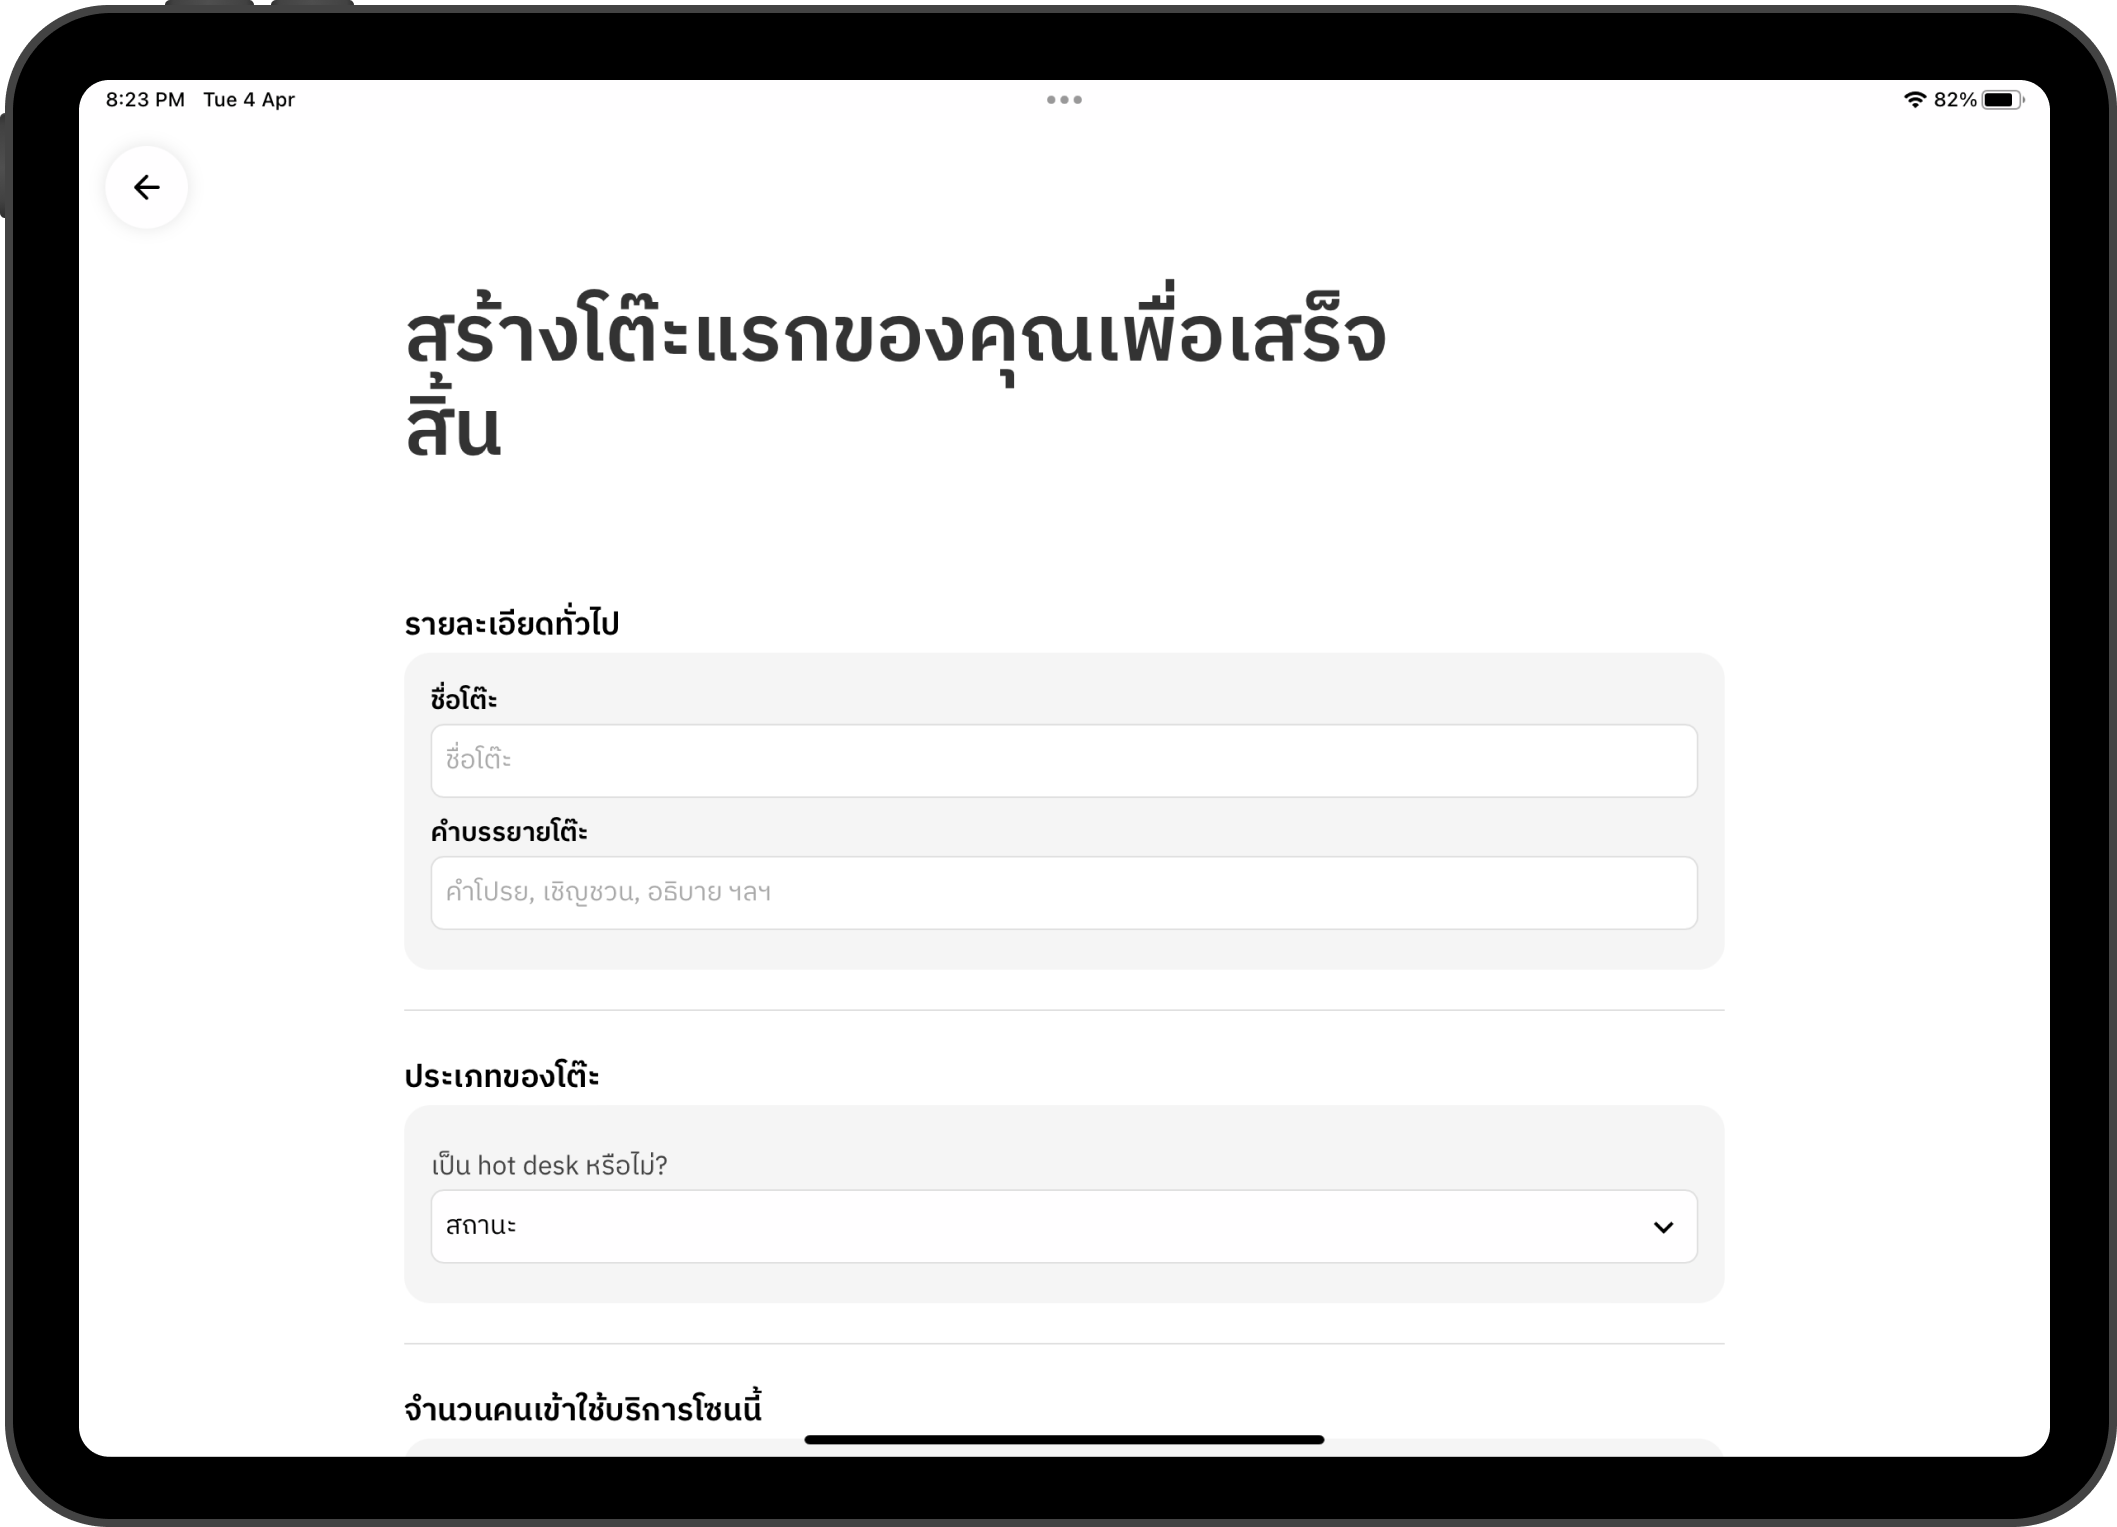
\includegraphics[width=5.5in]{./image/Flowider_desk_1.png}
    \end{center}
    \caption[Flowider desk 1]{หน้าระบุรายระเอียดของโต๊ะ}
    \label{fig:Flowider_desk_1}
\end{figure}
\begin{figure}[ht]
    \begin{center}
    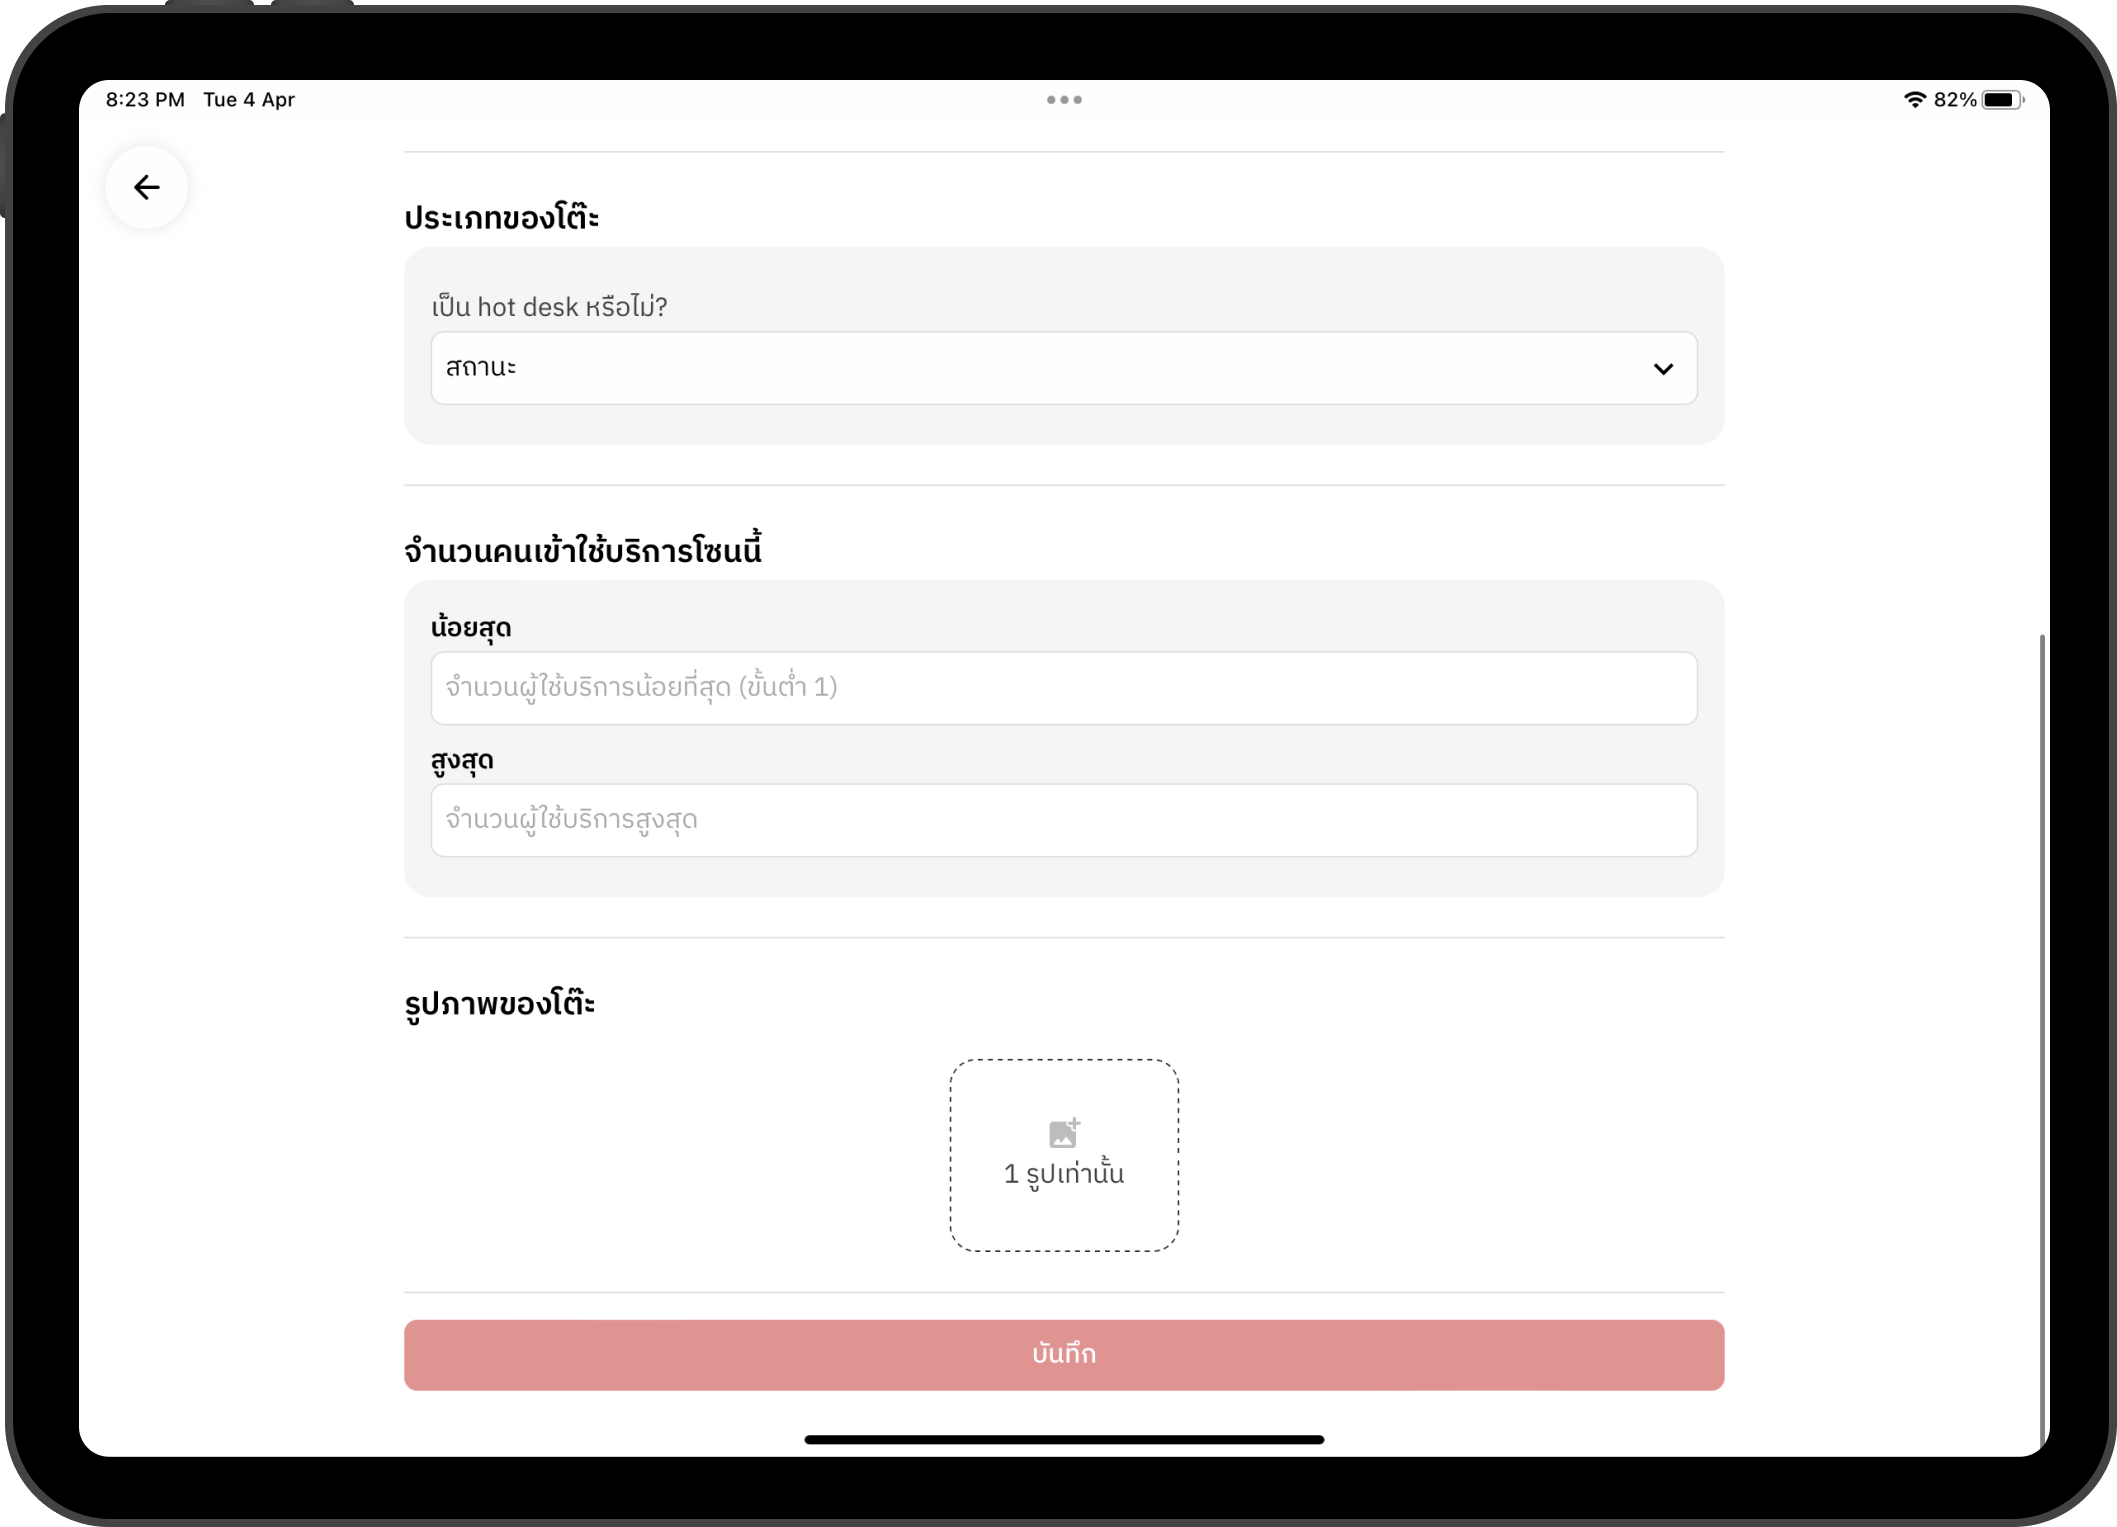
\includegraphics[width=5.5in]{./image/Flowider_desk_2.png}
    \end{center}
    \caption[Flowider desk 2]{หน้าระบุรายระเอียดของโต๊ะ (ต่อ)}
    \label{fig:Flowider_desk_2}
\end{figure}

\chapter{\ifproject%
\ifenglish Experimentation and Results\else การทดลองและผลลัพธ์\fi
\else%
\ifenglish System Evaluation\else การประเมินระบบ\fi
\fi}

\section{การประเมินผลการใช้งาน}
ในส่วนของการประเมินผลการใช้งานแอปพลิเคชันของโครงงานนี้ เราได้แบ่งออกเป็น 2 ประเภท ได้แก่ การทดสอบฝั่ง Flowy (ผู้เช่า) และการทดสอบฝั่ง Flowider (โฮสต์)

\subsection{การทดสอบฝั่ง Flowy}
ทั้งหมด 2 รูปแบบ
\subsubsection{Heuristic Usability Test}
ดังที่กล่าวไว้ว่าโครงงานนี้ให้ความสำคัญกับ User Experience หรือประสบการณ์ของผู้ใช้งานเป็นหลัก เราจึงใช้วิธีการทดสอบแบบ Heuristic Usability Test เพื่อทดสอบและวัดความเข้าใจของผู้ใช้งานตามหลักการ Human-Computer Interaction (HCI)

โดยขั้นตอนวิธีการทดสอบ Heuristic Usability Test มีดังนี้
\begin{enumerate}
    \item เลือกกลุ่มเป้าหมายที่ต้องการใช้งาน Flowy ทั้งหมด 5 คนเป็นผู้ทดสอบ
    \item ให้ผู้ทดสอบใช้งานแอปพลิเคชันตามขั้นตอนหรือขอบเขตการทดสอบแต่ละส่วน โดยไม่มีการอธิบายขั้นตอนการใช้งานล่วงหน้าหรือแม้แต่ระหว่างการใช้งานว่าส่วนใดคืออะไรหรือทำหน้าที่อย่างไร กล่าวคือให้ผู้ทดสอบเผชิญการใช้งานเองทั้งหมดตาม brief
    \item เมื่อสิ้นสุดในแต่ละขอบเขตตาม brief จะให้ผู้ใช้งานลงคะแนนแต่ละส่วนผ่าน Google Form ในแต่ละคำถามเพื่อนำมาสรุปผล
\end{enumerate}
\subsubsection{Problem-Solution Fit}
ดังที่กล่าวไว้ว่าโครงงานนี้ยังให้ความสำคัญกับความสามารถการแข่งขันในเชิงธุรกิจด้วย เราจำใช้วิธีการทดสอบกับกลุ่มลูกค้าเป้าหมาย (customer segment) เพื่อให้รู้แน่ชัดว่าเมื่อผลิตภัณฑ์ของเราออกสู่ตลาดแล้วจะมีลูกค้าเข้ามาใช้บริการของเราอย่างแน่นอน

อย่างไรก็ตามรูปแบบของการทดสอบ Problem-Solution Fit นั้นไม่มีรูปแบบเฉพาะเจาะจงตายตัว ผู้สนใจทดสอบในรูปแบบนี้สามารถออกแบบวิธีการทดสอบด้วยตนเองได้ตามแต่ถนัด

โดยขั้นตอนวิธีการทดสอบ Problem-Solution Fit ในรูปแบบของ Flowy มีดังนี้
\begin{enumerate}
    \item ทำการสุ่มเลือกผู้ทำแบบสอบถามและสนใจจะใช้งาน Flowy (early adopter) ผ่านช่องทาง social media ทั้งหมด 20 คน แล้วติดต่อกลับ
    \item ส่งตัวต้นแบบแอปพลิเคชันของเราให้ early adopter ทั้งหมด 20 คนได้ลองใช้งานและสัมผัสประสบการณ์จำลอง
    \item รอรับความคิดเห็น (feedback) หลังจากใช้งานเสร็จสิ้น
\end{enumerate}

\subsection{การทดสอบฝั่ง Flowider}
ทั้งหมด 1 รูปแบบ
\subsubsection{Phone Interview}
ในส่วนของการทดสอบฝั่ง Flowider ผู้พัฒนาไม่สามารถทดสอบรูปแบบอื่นได้ เนื่องจากปัญหาการพัฒนาแอปพลิเคชันที่ล่าช้า จึงทำให้มีเวลาไม่เพียงพอสำหรับการเจรจาทางธุรกิจกับกลุ่มของ Flowider ซึ่งทำให้ไม่สามารถนำกลุ่ม Flowider เข้าสู่แพลตฟอร์มของเราและทำการทดสอบการใช้งานแอปพลิเคชันได้

อย่างไรก็ตามเราได้ทำการติดต่อผู้ประกอบการหรือเจ้าของพื้นที่ที่มีศักยภาพที่จะเข้ามาอยู่บนแพลตฟอร์มของเราทั้งหมดรวม 10 รายด้วยกัน ซึ่งสามารถแบ่งประเภทได้ดังนี้
\begin{enumerate}
    \item คาเฟ่, ร้านกาแฟ ทั้งหมด 3 ราย
    \item โรงแรม, โฮสเทล ทั้งหมด 4 ราย
    \item สถานที่ส่วนบุคคล, บ้าน, โคเวิร์กกิ้งสเปซ ทั้งหมด 3 ราย
\end{enumerate}

\section{ผลการประเมินการใช้งาน}
\subsection{ผลการทดสอบฝั่ง Flowy}
\textbf{ผลการทดสอบ Heuristic Usability Test}
\begin{figure}[h]
    \begin{center}
    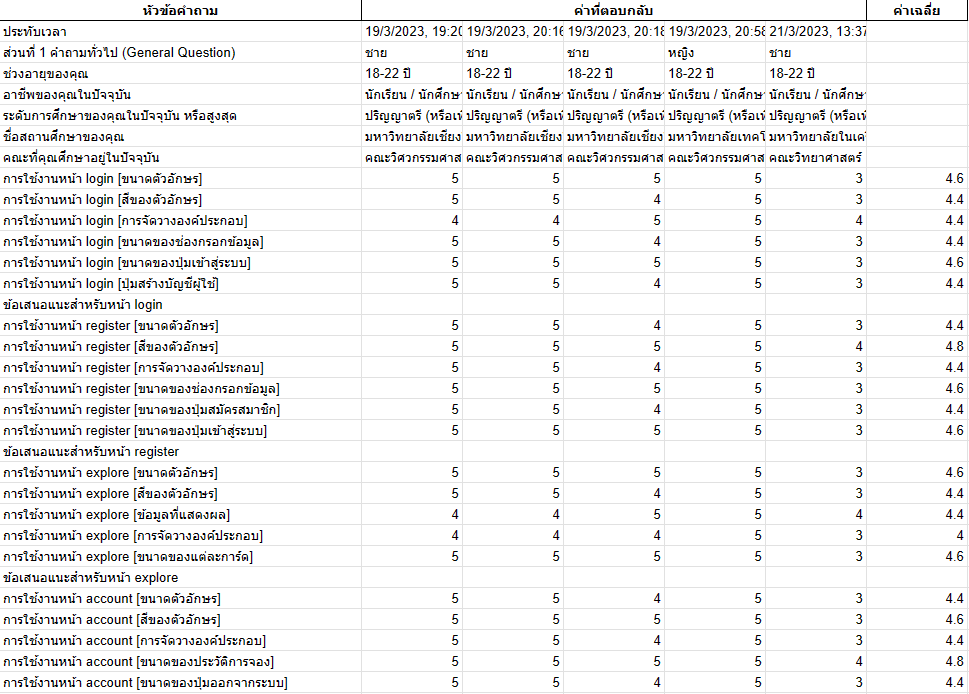
\includegraphics[width=\linewidth]{./image/heuristic_usability_test.png}
    \end{center}
    \caption[Heuristic Usability Test]{รูปภาพผลการทดสอบ Heuristic Usability Test บางส่วน}
    \label{fig:heuristic_usability_test}
\end{figure}

หลังจากได้ทำการทดสอบกับกลุ่มเป้าหมาย 5 คน ผลปรากฎว่า คะแนนเฉลี่ยที่ได้ในแต่ละหัวข้อการทดสอบนั้นอยู่ในช่วง 4 - 4.8 คะแนน ซึ่งสำหรับเกณฑ์ของผู้พัฒนานั้นถือว่าอยู่ในเกณฑ์ที่ดีมาก โดยคะแนนความเข้าใจเฉลี่ยรวมในทุก component ทั้งหมดคือ 4 คะแนนจาก 5 คะแนน และในส่วนของความพึงพอใจจากการใช้งานทั้งหมดคือ 9 คะแนนจาก 10 คะแนน จากช่องตารางสีเขียวดังรูป

\begin{figure}[h]
    \begin{center}
    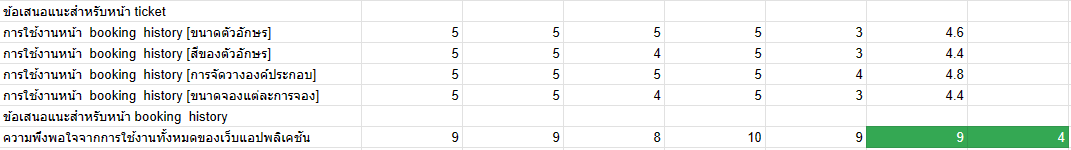
\includegraphics[width=\linewidth]{./image/heuristic_result.png}
    \end{center}
    \caption[Heuristic result]{รูปภาพผลคะแนนการทดสอบเฉลี่ยรวมในช่องตารางสีเขียว}
    \label{fig:heuristic_result}
\end{figure}

จึงสามารถสรุปได้ว่า ณ เวลาที่ได้ทำการทดสอบกับผู้ทดสอบ  User Flow ที่ผู้ใช้งานได้สัมผัสและได้มีประสบการ์ใช้งานจากแอปพลิเคชันของเรา สามารถสื่อสารให้ผู้ใช้งานเข้าใจใน functionality ของส่วนต่าง ๆ ได้เป็นอย่างดี

\subsubsection{ผลการทดสอบ Problem-Solution Fit Test}
จากการทดสอบ Problem-Solution Fit Test กับ early adopter ทั้งหมด 20 คน มีผู้ที่ลงความเห็นว่าจะใช้งาน Flowy แน่นอนหลังจากเปิดตัว public launch ถึง 17 คน ซึ่ง 3 คนที่เหลือที่เลือกจะไม่ใช้งานต่อได้ให้เหตุผลว่า ``อยากให้มีจำนวนของ Flowider มากกว่านี้เพื่อจะได้มีตัวเลือกที่หลากหลายในการเข้าใช้บริการ'' หรือบ้างก็ว่า ``ผลิตภัณฑ์ยังมีความยุ่งยากในการใช้งานมากเกินไปสำหรับตน''
\begin{figure}[h]
    \begin{center}
    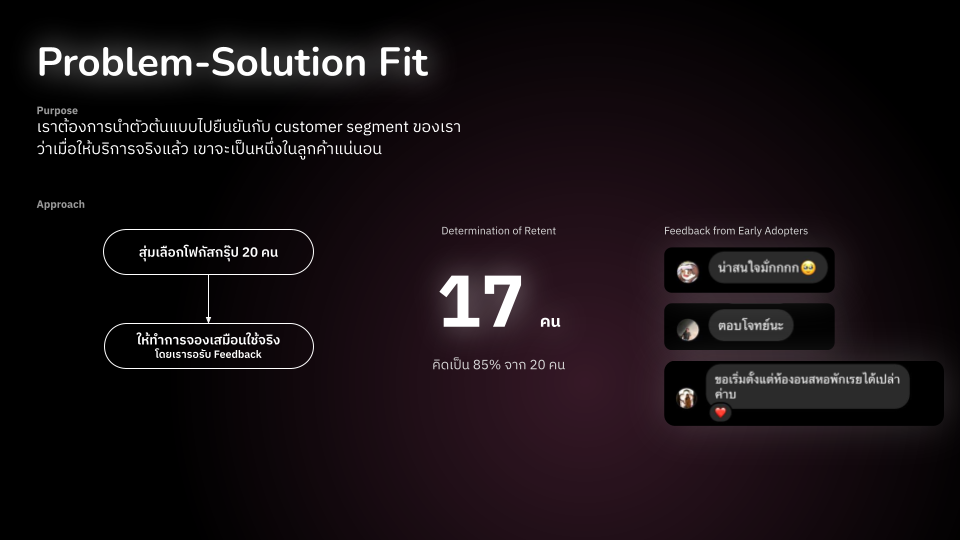
\includegraphics[width=\linewidth]{./image/Problem-Solution_Fit.png}
    \end{center}
    \caption[Problem-Solution Fit]{ผลการทดสอบ Problem-Solution Fit}
    \label{fig:Problem-Solution_Fit}
\end{figure}

\subsection{ผลการทดสอบฝั่ง Flowider}
จากการโทรศัพท์ติดต่อเจรจา มีผู้ประกอบการและเจ้าของพื้นที่สนใจที่จะเป็นส่วนหนึ่งกับแพลตฟอร์มเพียง 3 รายจาก 10 ราย โดยส่วนใหญ่ให้เหตุผลประกอบว่าไม่สะดวกหรือเป็นห่วงเรื่องความปลอดภัยของข้อมูลของผู้ใช้งาน

อย่างไรก็ตามผู้ประกอบการ 3 รายที่มีแนวโน้มจะเข้าร่วมกับแพลตฟอร์ทมของเรานั้นก็มีเงื่อนไขพ่วงในการเข้าร่วมด้วยเช่นกัน โดยต้องการให้ทีมผู้พัฒนาทำจดหมายขออนุญาตอย่างเป็นทางการผ่านภาควิชาวิศวกรรมคอมพิวเตอร์เพื่อขออนุญาตดำเนินการและหาผู้รับผิดชอบหากเกิดเหตุไม่พึงประสงค์ใด ๆ ขึ้น

ทั้งหมดนี้จากข้อจำกัดเรื่องของเวลาที่มีอยู่น้อย ทีมผู้พัฒนาจึงไม่ได้ดำเนินการต่อในช่วงก่อนการนำเสนอการสอบปลายภาค แต่จะดำเนินการต่อหลังจากการสอบปลายภาคเสร็จสิ้นต่อไป
\begin{figure}[h]
    \begin{center}
    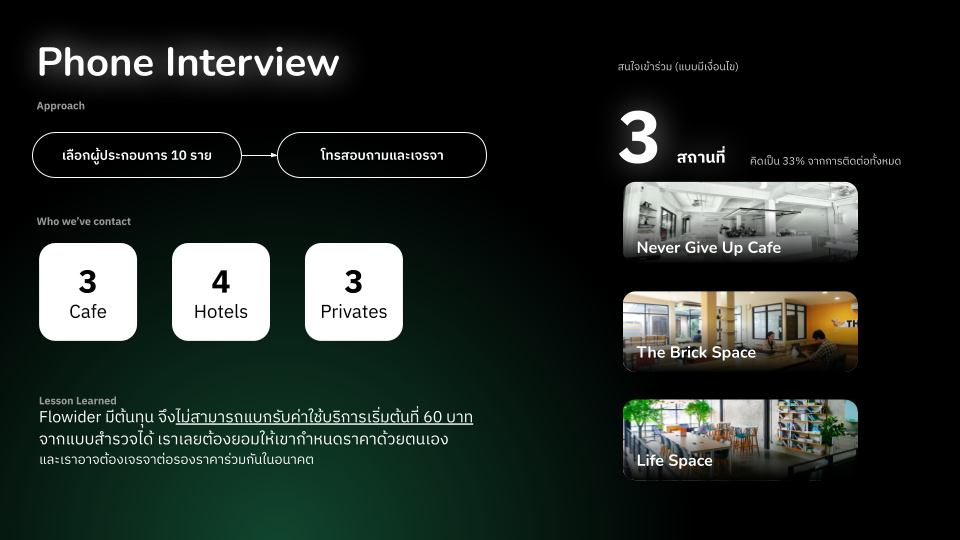
\includegraphics[width=\linewidth]{./image/Phone_interview.png}
    \end{center}
    \caption[Phone Interview]{Phone Interview}
    \label{fig:Phone_interview}
\end{figure}

\ifproject
\chapter{\ifenglish Conclusions and Discussions\else บทสรุปและข้อเสนอแนะ\fi}

\section{\ifenglish Conclusions\else สรุปผล\fi}

โครงงาน Flowy: Rent hourly for reading \& co-working จัดทำขึ้นเพื่อแก้ไขปัญหาพื้นที่หรือที่นั่งไม่เพียงพอในการทำกิจกรรมต่าง ๆ ตามความต้องการของผู้ใช้งาน โดยโครงงานนี้สามารถแบ่งการสรุปออกมาได้ 2 หมวดหมู่ได้แก่ ด้านเทคนิคและด้านธุรกิจ

\subsubsection{ด้านเทคนิค}
ผลสรุปของด้านเทคนิคนั้นถือว่าทีมผู้พัฒนานั้นสามารถทำออกมาได้สมบูรณ์แบบตามความต้องการ ทั้งในเรื่อง UI/UX ก็ดีหรือ functionality ของตัวแอปพลิเคชันทั้ง 2 ก็ดี แน่นอนว่ามีรายละเอียดบางจุดที่สามารถพัฒนาให้ดีขึ้นหรือแก้ไขเพิ่มเข้าไปภายหลังได้ แต่เนื่องด้วยข้อจำกัดของเวลาทางผู้พัฒนาจึงตั้งสินใจทำ feature ที่สำคัญเท่าที่จำเป็นก่อน แม้ว่าทีมผู้พัฒนาจะมีแนวความคิดการพัฒนาผลิตภัณฑ์ออกมาในรูปแบบของ Minimum Viable Product (MVP) อยู่แล้ว แต่ผลลัพธ์ที่ตั้งใจทำออกมาก็เกินจุดที่จะเรียกว่า MVP ไปอยู่พอสมควร

\subsubsection{ด้านธุรกิจ}
ผลสรุปของด้านธุรกิจนั้นถือว่าบรรลุเป้าหมายเพียง 70\% เท่านั้น โดย 30\% ที่เหลือที่ไม่สามารถบรรลุได้นั้นคือการให้โฮสต์ (Flowider) เข้ามาใช้บริการในฐานะ contributor ให้ได้มากที่สุดเพื่อที่จะได้ทำการ public launch ต่อไปตามแผนที่วางไว้ในตอนต้น แต่เนื่องด้วยระยะเวลาของการพัฒนาที่พยายามจะส่งมอบ feature ต่าง ๆ ที่จำเป็นให้ฝั่ง Flowider ให้ได้มากที่สุด จึงทำให้กินระยะเวลาของการทดสอบดังกล่าวไปโดยสรุปทั้งหมด ณ ปัจจุบันที่รายงานฉบับนี้ได้เขียนอยู่ แอปพลิเคชันทั้ง 2 นั้นสามารถใช้การทุก feature ที่จำเป็นและเป็นพื้นฐานได้อย่างครบถ้วนและสามารถที่จะแก้ไขหรือพัฒนาต่อไป โดยในอนาคตทางผู้พัฒนามีความตั้งใจที่จะพัฒนาต่อและทำให้ Flowy นี้สามารถเป็นธุรกิจที่เข้ามาตอบโจทย์ความต้องการของผู้ที่มองหาพื้นที่ในการทำงาน, อ่านหนังสือ หรือทำกิจกรรมอื่น ๆ ต่อไปตามแผนที่วางไว้ในตอนต้น

\section{\ifenglish Challenges\else ปัญหาที่พบและแนวทางการแก้ไข\fi}

\subsubsection{Flowider มีน้อย เนื่องด้วยเหตุผลทางธุรกิจ}
เนื่องด้วย Flowy เป็นแอปพลิเคชันแพลตฟอร์ม จึงหมายความว่าเราต้องทำงานกับ stakeholder มากกว่า 1 ฝ่าย ซึ่งในที่นี่ Flowy ต้องทำงานกับ 2 ฝ่ายหลักด้วยกันคือฝั่งของ Flowy (ผู้เช่า) และ Flowider (โฮสต์) โดยในส่วนของ Flowider นั้นเป็นข้อจำกัดของโครงงานนี้ เนื่องจากทีมผู้พัฒนาได้ทำการติดต่อผ่านการโทรศัพท์ไปติดต่อเจรจากับเจ้าของพื้นที่นั้น ๆ เพื่อเชิญชวนให้เขาเข้ามาเป็นส่วนหนึ่งกับเรา

แต่ผลการเจรจานั้นส่วนใหญ่แล้วจะไม่ประสบความสำเร็จเนื่องจากปัญหาเรื่องความเชื่อใจและความปลอดภัยของข้อมูลส่วนบุคคลที่จะเข้ามาสู่แพลตฟอร์มของเรา หรือในความเห็นผู้พัฒนาเองก็คิดว่าเนื่องด้วยเรายังมีสถานะเป็นนักศึกษาอยู่จึงทำให้ความเชื่อมั่นหรือความมั่นใจที่จะเข้าร่วมนั้นมีไม่พอที่จะทำให้ Flowider ตัดสินใจเข้าร่วม

โดยแนวทางวิธีการแก้ไขปัญหานี้คือ เราจำเป็นต้องหาผู้ที่มีเงื่อนไขในการเข้าร่วมน้อยกว่านี้ ซึ่งอาจเปลี่ยนจากการเชิญชวนกลุ่มสถานที่ที่มีอุปสงค์เยอะอยู่แล้ว เช่น ร้านกาแฟ, โคเวิร์กกิ้งสเปซ ฯลฯ เป็น กลุ่มสถานที่ส่วนบุคคล เช่น บ้านหรือคอนโดมิเนียมแทน เพื่อให้การปล่อยเช่าของเขาสร้างรายได้นั้นลดกำแพงเงื่อนไขลง จนเมื่อเรามี Flowider ประเภทนี้มากเพียงพอแล้ว เราจึงจะมีเสียงในการต่อรองหรือเชิญชวนกลุ่มสถานที่อื่นอย่างร้านกาแฟ, โคเวิร์กกิ้งสเปซ เข้ามาบนแพลตฟอร์มของ Flowy

และอีกแนวทางหนึ่งคือควรเผื่อเวลาไว้สำหรับการเข้าไปเจรจาตัวต่อตัวด้วย ซึ่งทางทีมผู้พัฒนาไม่ได้เผื่อเวลาในส่วนนี้เพียงพอ

\subsubsection{ระบบ Search \& Filter}
เดิมแล้ว Flowy ตั้งใจที่จะทำระบบ Search \& Filter อย่างที่แพลตฟอร์มอื่น ๆ ที่มีลักษณะใกล้เคียงกันมี ซึ่งเมื่อเราทำออกมาแล้วแต่ยังมีจำนวนของ Flowider บนแพลตฟอร์มไม่เพียงพอ เราพบว่าทำให้ประสบการณ์การใช้งานนั้นไม่ค่อยดีเพราะเมื่อทำการค้นหาแล้วบางครั้งก็ไม่พบสถานที่ที่ตรงกับความต้องการ เราจึงแก้ไขปัญหานี้เฉพาะหน้าด้วยการเพิ่มส่วนทักทายผู้ใช้งานไปก่อน จนเมื่อเรามี Flowider มากเพียงพอแล้วจึงจะเปิดใช้ feature นี้อีกครั้งหนึ่ง
\begin{figure}[h]
    \begin{center}
    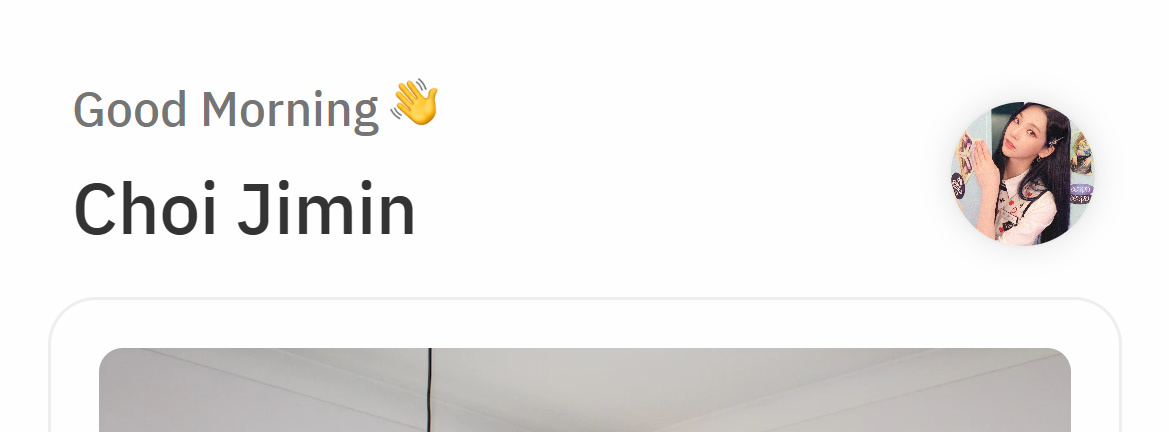
\includegraphics[width=4in]{./image/welcome_bar.png}
    \end{center}
    \caption[Welcome bar]{รูปภาพส่วนทักทายผู้ใช้งานดังกล่าว}
    \label{fig:welcome_bar}
\end{figure}

\section{\ifenglish%
Suggestions and further improvements
\else%
ข้อเสนอแนะและแนวทางการพัฒนาต่อ
\fi
}
ในส่วนของ Flowy และ Flowider ควรที่จะพัฒนา UI/UX ให้ดีขึ้นกว่านี้เพื่อการใช้งานที่มีประสิทธิภาพ หน้าตา interface ที่สวยงาม และมอบประสบการณ์การใช้งานที่ดีให้กับ user โดยอาศัยการเข้าไปทดสอบและพูดคุยถึงปัญหาและความต้องการของ user ให้สม่ำเสมอและนำหลักการออกแบบมาใช้

ซึ่งจากประเด็นดังกล่าว เรานำมาต่อยอดในเรื่องของการให้บริการของเราที่ปัจจุบันนั้นมีบริษัทหลายแห่งที่มีระบบ Point-of-Sell (POS) เช่น Grab, Lineman ฯลฯ ซึ่งหากเราจะเป็นหนึ่งในบริษัทเหล่านั้นที่ต้องการให้ Flowider ใช้งาน POS ของเราอีกหนึ่งเครื่อง อาจเป็นตัวเลือกที่ไม่ค่อยดีนักเพราะผู้ใช้งานต้องทำงานกับอุปการณ์มากชิ้น โดยอาจารย์พฤษภ์ บุญมาได้ให้คำแนะนำว่าเราควรที่จะไป integrate หรือเชื่อมต่อระบบกับผู้ให้บริการเหล่านั้นดังที่กล่าวสักหนึ่งเจ้า ให้เป็นความร่วมมือทางธุรกิจที่สามารถสร้างประโยชน์ได้ทุกฝ่าย ซึ่งเราก็ไม่จำเป็นต้องให้ Flowider ใช้ระบบ POS ของเราอีกแล้ว ลดต้นทุนการผลิตลง, พันธมิตรธุรกิจของเราก็ได้เพิ่มโอกาสทางธุรกิจใน sector อื่น ๆ และสุดท้ายผู้ใช้งานก็มีประสบการณ์ใช้งานที่ดี ไม่จำเป็นต้องทำงานกับอุปกรณ์หลายชิ้นอีกต่อไป

\fi

\bibliography{flowyReport}

\ifproject
\normalspacing
\appendix
\chapter{คู่มือการใช้งานระบบ Flowy}

\section{Login}
ขั้นตอนการเข้าสู่ระบบ ผู้ใช้งานต้องทำการกรอก username, password หลังจากนั้นกดปุ่ม \textbf{เข้าสู่ระบบ} หากผู้ใช้งานยังไม่มีบัญชีผู้ใช้งาน สามารถกด \textbf{สร้างบัญชีผู้ใช้} ได้

\section{Register}
ขั้นตอนการสร้างบัญชีผู้ใช้ ผู้ใช้งานต้องทำการกรอกข้อมูลดังต่อไปนี้
\begin{itemize}
    \item ชื่อ - นามสกุล
    \item อีเมล
    \item เบอร์โทรศัพท์
    \item รหัสผ่าน  
\end{itemize}
หากกรอกข้อมูลครบถ้วนกดปุ่มสมัครสมาชิก สำหรับผู้ใช้งานมีบัญชีอยู่แล้วสามารถกดปุ่ม \textbf{มีบัญชีอยู่แล้ว? เข้าสู่ระบบ} ได้เลย

\section{Account}
แสดงข้อมูลส่วนตัวของผู้ใช้งาน หากผู็ใช้งานต้องการทราบรายละเอียดการจองที่ผ่านมาสามารถกดได้ที่ \textbf{ประวัติการจอง} หากต้องการออกจากระบบผู้ใช้สามาถกดได้ที่ปุ่ม \textbf{ออกจากระบบ}

\section{Explore}
จะมีการแสดงผลในอยู่สองส่วนคือ สเปซที่ให้บริการ และโปรไฟล์
\begin{itemize}
    \item สเปซที่ให้บริการ ผู้ใช้บริการสามารถเลือกสเปซที่คุณต้องการได้จากการอ่านรายละเอียดที่แสดงผล โดยมีข้อมูลที่แสดงผลลดังต่อไปนี้
    \begin{itemize}
        \item ชื่อสเปซ
        \item เวลาเปิด - ปิดสเปซ
        \item ที่อยู่ของสเปซ
        \item ราคาค่าใช้งานเปซต่อชั่วโมง
        \item ความเฉพาะเจาะจง        
    \end{itemize}
    \item โปรไฟล์ ผู้ใช้บริการสามารถเข้ามาดูข้อมูลส่วนตัว และประวัติการจองสเปซได้จากส่วนนี้ 
\end{itemize}

\section{Place information}
จะแสดงข้อมูลรายละเอียดทั้งหมดของสเปซนั้น ๆ โดยจะแสดงข้อมูลดังต่อไปนี้
\begin{itemize}
    \item ชื่อสเปซ
    \item เวลาเปิด - ปิดสเปซ
    \item ที่อยู่ของสเปซ
    \item ราคาค่าใช้งานเปซต่อชั่วโมง
    \item สิ่งอำนวยความสะดวก
    \item ความเฉพาะเจาะจง
\end{itemize}
เมื่อผู้ใช้อ่านรายละเอียดแล้วต้องการจองสเปซ สามารถกดปุ่ม \textbf{จอง} ด้านล่างของหน้าจอเพื่อเข้าสู้ขั้นตอนของการจอง หากไม่ต้องกานจองสเปซนั้นแล้ว
ผู้ใช้งานสามารถกดปุ่ม \textbf{ย้อนกลับ} ได้ที่บนมุมขวาของหน้าจอ

\section{Booking  customer amount}
ผู้ใช้ต้องทำการระบบุจำนวนผู้เข้าใช้บริการสเปวนนั้น เมื่อผู้ใช้งานทำการเลือกจำนวนผู้ใช้งานเรียนร้อยแล้ว ผู้ใช้งานต้องกดปุ่ม \textbf{ถัดไป} เพื่อเข้าสู้หน้าเลือกรูปแบบโต๊ะ/ที่นั่ง
หากไม่ต้องการกลับสู่หน้าที่แล้วผู้ใช้งานสามารถกดปุ่ม \textbf{ย้อนกลับ} ได้ที่บนมุมขวาของหน้าจอ

\section{Booking desk}
ผู้ใช้ต้องทำการเลือกโต๊ะ/ที่นั่งที่แสดงผลได้ตามความต้องการ หลังจากนั้นกดปุ่ม \textbf{เลือก} ระบบจะพาไปสู่หน้าเลือกเวลาเข้าใช้บริการ
หากไม่ต้องการกลับสู่หน้าที่แล้วผู้ใช้งานสามารถกด \textbf{ย้อนกลับ} ได้ที่บนมุมขวาของหน้าจอ

\section{Booking time slot}
ผู้ใช้งานต้องทำการระบุเวลาที่ต้องการใช้งานโดยสามารถกดเลือกเวลาที่ว่าง เมื่อผู้ใช้กดเลือกเวลาที่ต้องการใช้งานสีที่แสดผลจะถูกเปลี่ยนเป็นสีแดง หากช่วงเวลาที่ไม่ว่างสล๊อตที่แสดงผลจะแสดงผลในสีเทาและไม่สามารถกดได้ \\
เมื่อผู้ใช้งานเลือกเวลาที่ต้องเข้างานเรียบร้อย กดปุ่มจองเลยตอนนี้ระบบจะพาไปสู่หน้าชำระค่าบริการ หากไม่ต้องการกลับสู่หน้าที่แล้วผู้ใช้งานสามารถกดปุ่มย้อนกลับได้ที่บนมุมขวาของหน้าจอ

\section{Payment}
สำหรับการจ่ายเงินจะมีส่วนแสดงผลอยู่สองส่วน คือ รายละเอียดค่าใช้บริการ และการชำระค่าบริการ
\begin{itemize}
    \item รายละเอียดค่าใช้บริการจะแสดงราคาที่ผู้ใช้บริการต้องททำการชำระโดยจะมีรายละเอียดดังนี้
    \begin{itemize}
        \item ค่าใช้บริการต่อชั่วโมง
        \item จำนวนผู้ใช้บริการสเปซ
        \item จำนวนชั่วโมงในการใช้บริการสเปซ        
    \end{itemize}
    \item การชำระค่าบริการ จะมีอยู่สองวิธี
    \begin{itemize}
        \item บัตรเครดิต/เดบิต
        \item พร้อมเพย์ QR        
    \end{itemize}
\end{itemize}
เมื่อชำระค่าบริการเรียบร้อยละบบจะพาไปสู่หน้าตั๋ว

\section{Ticket}
จะแสดงข้อมูลรายละเอียดการจองทั้งหมดโดยจะมีรายละเอียดที่แสดงผลดังนี้
\begin{itemize}
    \item ชื่อสเปซ และที่อยู่ของสเปซ
    \item วันที่จอง
    \item จำนวนชั่วโมงที่จอง
    \item QR code สำหรับการยืนยันข้อมูล
\end{itemize}
เมื่อผู้ใช้งานต้องการเดินทางไปที่สเปซสามารถกดปุ่ม \textbf{นำทางด้วย google maps} หรือถ้าผู้ใช้งานต้องการกลับสู่หน้าหลัก สามารถกดปุ่ม \textbf{กลับสู่หน้าหลัก} ได้

\chapter{คู่มือการใช้งานระบบ Flowider}

\section{Login}
ขั้นตอนการเข้าสู่ระบบ ผู้ใช้งานต้องทำการกรอก username, password หลังจากนั้นกดปุ่ม \textbf{เข้าสู่ระบบ} หากผู้ใช้งานยังไม่มีบัญชีผู้ใช้งาน สามารถกด \textbf{สร้างบัญชีผู้ใช้} ได้

\section{Register}
ขั้นตอนการสร้างบัญชีผู้ใช้ ผู้ใช้งานต้องทำการกรอกข้อมูลดังต่อไปนี้
\begin{itemize}
    \item ชื่อ - นามสกุล
    \item อีเมล
    \item เบอร์โทรศัพท์
    \item ชื่อธนาคาร
    \item หมายเลขบัญชีธนาคาร    
    \item รหัสผ่าน  
\end{itemize}
หากกรอกข้อมูลครบถ้วนกดปุ่มสมัครสมาชิก สำหรับผู้ใช้งานมีบัญชีอยู่แล้วสามารถกดปุ่ม \textbf{มีบัญชีอยู่แล้ว? เข้าสู่ระบบ} ได้เลย

\section{Dashboard}
หลังจากทำการเข้าสู้ระบบสำเร็จ จะหน้าแสดงลิตส์ของสเปซที่ผู้ให้บริการที่ได้ทำการลงทะเบียนไว้กับทาง flowy เมื่อกดเข้าสู่สเปซนั้น ๆ จะพบกับข้อมูลลการบุ๊กกิ้งของผู้ใช้บริการที่ได้ทำการจองเข้ามาในแต่ละวัน \\
หากผู้ให้บริการต้องการเพิ่มสเปซสามารถทำได้ด้วยการกดปุ่มจัดการที่แผงควบคุมทางด้านล่างตรงกลาง (รูปบ้าน) และถ้าผู้ใช้บริการต้องการดูข้อมูลส่วนตัวสามารถดูได้จากการกดปุ่มรูปตั้งค่า (รูปฟันเฟือง)

\section{Schedule}
หน้าแสดงบุ๊กกิ้งของสเปซนั้น ๆ ในแต่ละวัน หากต้องการย้อนกลับสู้หน้า dashboard สามารถทำได้โดยการกดปุ่ม \textbf{ย้อนกลับ} ที่บนมุมขวาของหน้าจอ

\section{Management}
หน้าจัดการสเปซ เป็นหน้าที่ผู้ให้บริการสามารถทำการเพิ่มสเปซ หรือทำการแก้ไขข้อมูลของสเปซได้ โดยการเพิ่มสเปซผู้ให้บริการสามารถทำได้โดยการกดปุ่ม \textbf{สร้างสเปซใหม่ +} และถ้าผู้ให้บริการต้องการแก้ไขข้อมูลของแต่ละสเปซที่ได้ทำการลงทะเบียนไว้ สามารถทำได้โดยการกดปุ่ม \textbf{แก้ไข} ที่มุมขวาล่างของแต่ละสเปซ \\
หากผู้ให้บริการต้องการลิตส์ของสเปซที่ได้ทำการลงทะเบียนสามารถกดที่แผงควบคุมทางด้านล่างด้านซ้าย (รูปปฏิทิน) และถ้าผู้ใช้บริการต้องการดูข้อมูลส่วนตัวสามารถดูได้จากการกดปุ่มรูปตั้งค่า (รูปฟันเฟือง)

\section{Add place}
เมื่อกดปุ่ม \textbf{สร้างสเปซใหม่ +} ระบบจะพาไปสู้หน้าเตรียมข้อมูลเพื่อใช้ในการลงทะเบียน มีขั้นตอนอยู่สองส่วนหลัก คือ ส่วนของการอธิบายเกี่ยวกับพื้นที่ของคุณ และส่วนของการเตรียมความพร้อมสำหรับโต๊ะแรก โดยมีข้อมูลที่ต้องเตรียมดังนี้
\begin{itemize}
    \item ข้อมูลเกี่ยวกับสเปซของคุณ
    \item ข้อมูลที่นั่งในสเปซของคุณ
\end{itemize}
หลังจากเตรียมข้อมูลเสร็จแล้วกดปุ่มกำเนินการต่อเพื่อทำการลงทะเบียนโดยทำการข้อมูลที่ได้บอกในขั้นตอนการเตรียมข้อมูลในข้างต้น เริ่มจาก ประเภทสเปซของคุณ, รายละเอียดของสเปซ, ความเฉพาะเจาะจง, สิ่งอำนวยความสะดวก, รูปภาพสำหรับสเปซของคุณ, ตำแหน่งสเปซของคุณ? และประเภทโต๊ะที่มีในสเปซ หลังจากกรอกข้อมูลครบถ้วนผู้ให้บริการสามารถกดปุ่มสร้างสเปซเพื่อทำการสร้างสเปซ

\section{Edit place}
หน้าจัดการของมูลของสปซที่คุณลงทะเบียนไว้ โดยมีข้อมูลที่สามารถแก้ไขได้ดังนี้
\begin{itemize}
    \item รูปภาพของสเปซ
    \item ข้อมูลทั่วไป
    \begin{itemize}
        \item ชื่อสเปซ
        \item ที่อยู่
        \item ประเภทสเปซ        
    \end{itemize}
    \item เวลาทำการ
    \begin{itemize}
        \item เวลาเปิด
        \item เวลาปิด        
    \end{itemize}
    \item ราคาต่อชั่วโมง (บาท)
    \item ความเฉพาะเจาะจง
    \begin{itemize}
        \item สูบบุหรี่ได้
        \item ใช้เสียงดังได้
        \item เงียบพิเศษ
        \item บรรยากาศดี
    \end{itemize}
    \item สิ่งอำนวยความสะดวก
    \begin{itemize}
        \item ปลั๊กไฟ/ปลั๊กพ่วง
        \item อินเทอร์เนต
        \item ห้องน้ำ
        \item จอแสดงผล
        \item สาย HDMI/สายสำหรับแสดงผล
        \item การดูแลอันอบอุ่นจากเจ้าของ
        \item เครื่องปรับอากาศ
        \item ขนม/เครื่องดื่ม
        \item การรักษาความปลอดภัย
    \end{itemize}
    \item ประเภทของโต๊ะที่มีในสเปซ
    \begin{itemize}
        \item ชื่อของโต๊ะ
        \item คำบรรยายโต๊ะ
        \item ประเภทของโต๊ะ
        \item จำนวนคนเข้าใชเบริการในโซนนี้
        \item รูปภาพของโต๊ะ        
    \end{itemize}
\end{itemize}
โดยการแก้ไขข้อมูลผู้ให้บริการสามารถกดที่คำว่า \textbf{แก้ไข} ที่มุมบนขวาของแต่ละส่วนเพื่อทำการแก้ไขข้อมูล เมื่อทำการการแก้ไขข้อมูลเสร็จสิ้นต้องทำการกดปุ่ม \textbf{บันทึก} เพื่อยืนยันการแก้ไข หากไม่ต้องการแก้ไชช้อมูลในส่วนนั้น ๆ ผู้ให้บริการสามารถกดที่ปุ่ม \textbf{ย้อนกลับ} ได้ที่มุมขวาบนของแต่ละส่วน \\
เมื่อต้องการกลับสู้หน้าจัดการสเปซผู้ใช้งานสามารถกดปุ่ม \textbf{ย้อนกลับ} ได้ที่มุมบนขวา

\section{Setting}
หน้าแสดงรายละเอียดของผู้ให้บริการ โดยจะมข้อมูลที่แสดงผลดังต่อไปนี้
\begin{itemize}
    \item ชื่อผู้ให้บริการ (ชื่อจริง - นามสกุล)
    \item วันที่สมัครใช้บริการ
    \item อีเมล
    \item เลขที่บัญชี
    \item ชื่อธนาคาร
\end{itemize}
การแก้ไขข้อมูลสามารถทำได้โดยยการกดปุ่ม \textbf{แก้ไข} ที่บนมุมขวาเพื่อทำการแก้ไขข้อมูล เมื่อทำการแก้ไขข้อมูลเรียบร้อยสามารถกดปุ่ม \textbf{ยืนยันการแก้ไขข้อมูล} เพื่อบันทึก \\
การออกจากระบบผู้ให้บริการสามารถทำได้โดยการกดปุ่ม \textbf{ออกจากระบบ} \\
หากผู้ให้บริการต้องการลิตส์ของสเปซที่ได้ทำการลงทะเบียนสามารถกดที่แผงควบคุมทางด้านล่างด้านซ้าย   (รูปปฏิทิน) และถ้าผู้ใช้บริการต้องการเพิ่มสเปซสามารถทำได้ด้วยการกดปุ่มจัดการที่แผงควบคุมทางด้านล่างตรงกลาง (รูปบ้าน)


% Text for a section in the first appendix goes here.

% test ทดสอบฟอนต์ serif ภาษาไทย

% \textsf{test ทดสอบฟอนต์ sans serif ภาษาไทย}

% \verb+test ทดสอบฟอนต์ teletype ภาษาไทย+

% \texttt{test ทดสอบฟอนต์ teletype ภาษาไทย}

% \textbf{ตัวหนา serif ภาษาไทย \textsf{sans serif ภาษาไทย} \texttt{teletype ภาษาไทย}}

% \textit{ตัวเอียง serif ภาษาไทย \textsf{sans serif ภาษาไทย} \texttt{teletype ภาษาไทย}}

% \textbf{\textit{ตัวหนาเอียง serif ภาษาไทย \textsf{sans serif ภาษาไทย} \texttt{teletype ภาษาไทย}}}

% \url{https://www.example.com/test_ทดสอบ_url}

% \chapter{\ifenglish Manual\else คู่มือการใช้งานระบบ\fi}

% Manual goes here.


%% Display glossary (optional) -- need glossary option.
\ifglossary\glossarypage\fi

%% Display index (optional) -- need idx option.
\ifindex\indexpage\fi

\begin{biosketch}
\begin{center}
  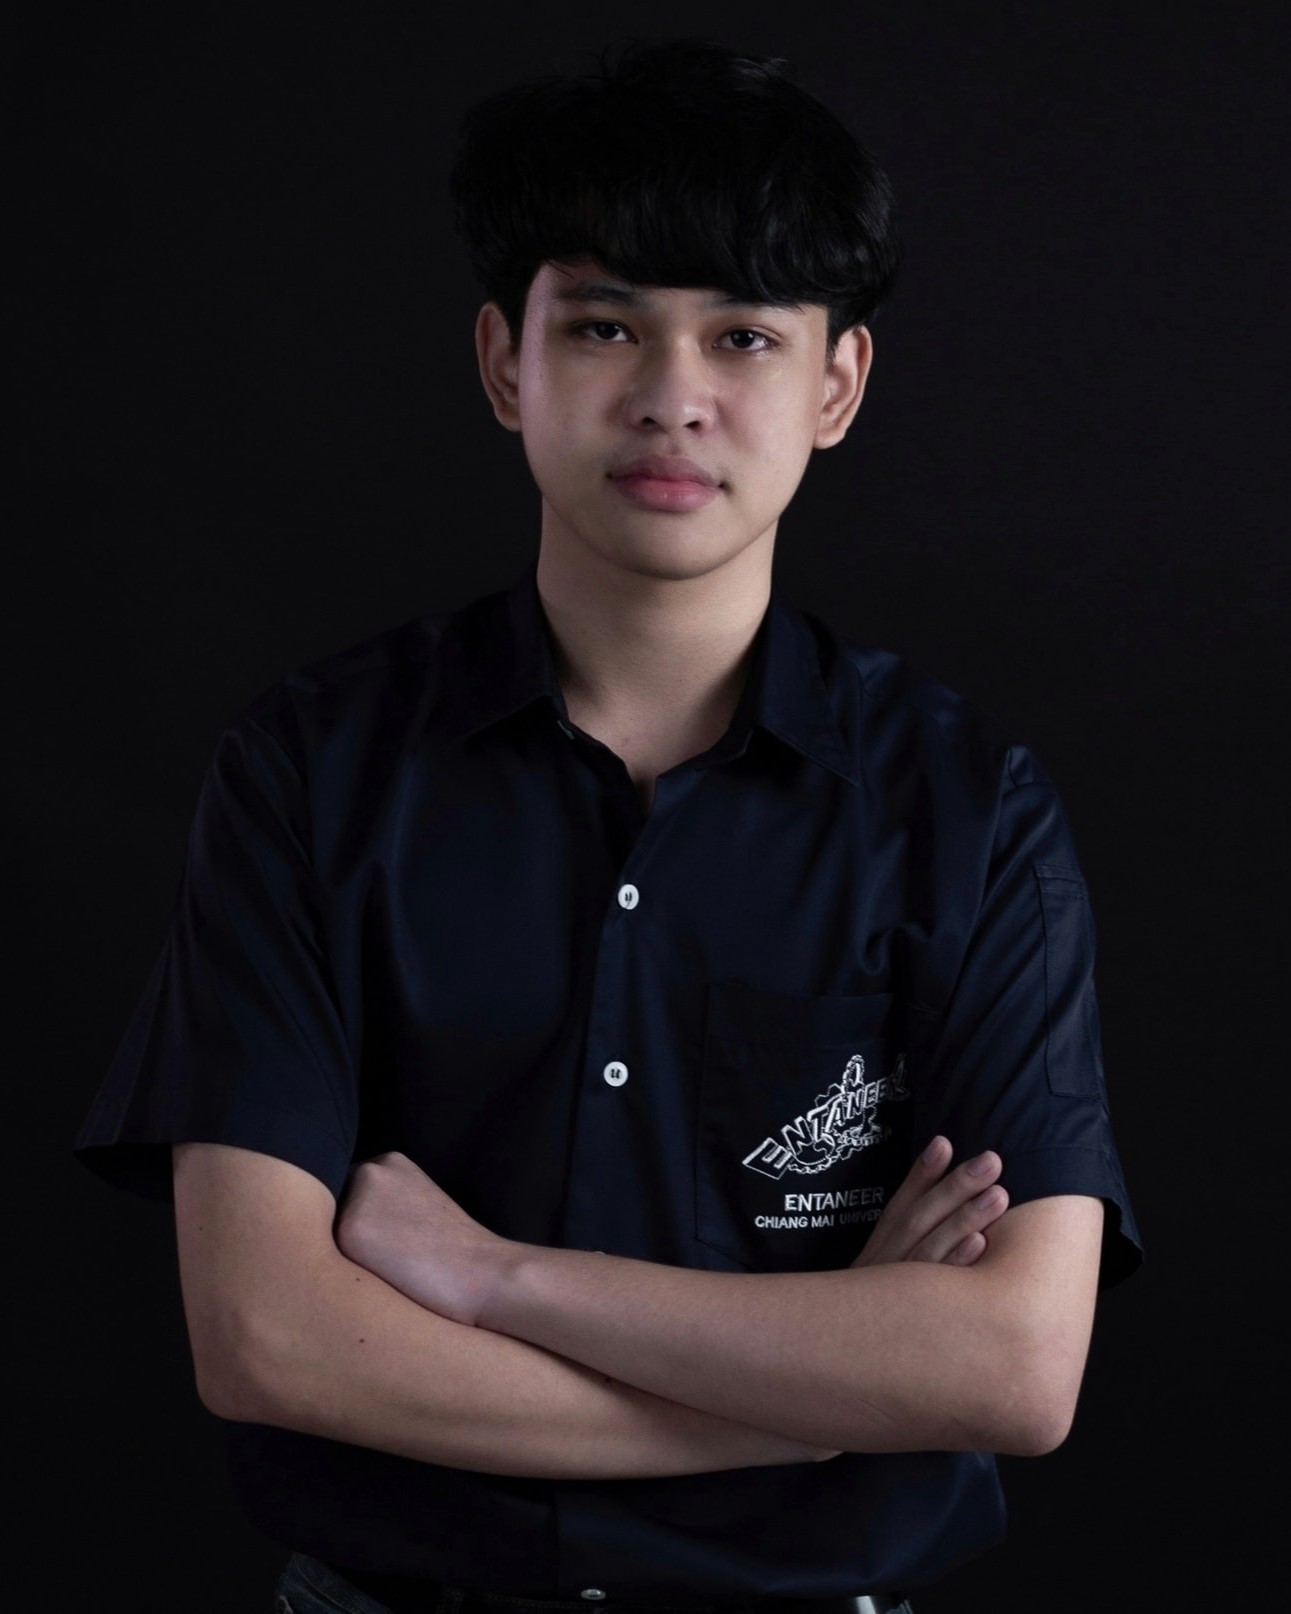
\includegraphics[width=1.5in]{./image/profile_bank.jpg}
\end{center}
นายชนาธิป สงจันทึก นักศึกษาชั้นปี ที่ 4 คณะวิศวกรรมศาสตร์ สาขาวิศวกรรมคอมพิวเตอร์ มหาวิทยาลัยเชียงใหม่
\begin{center}
  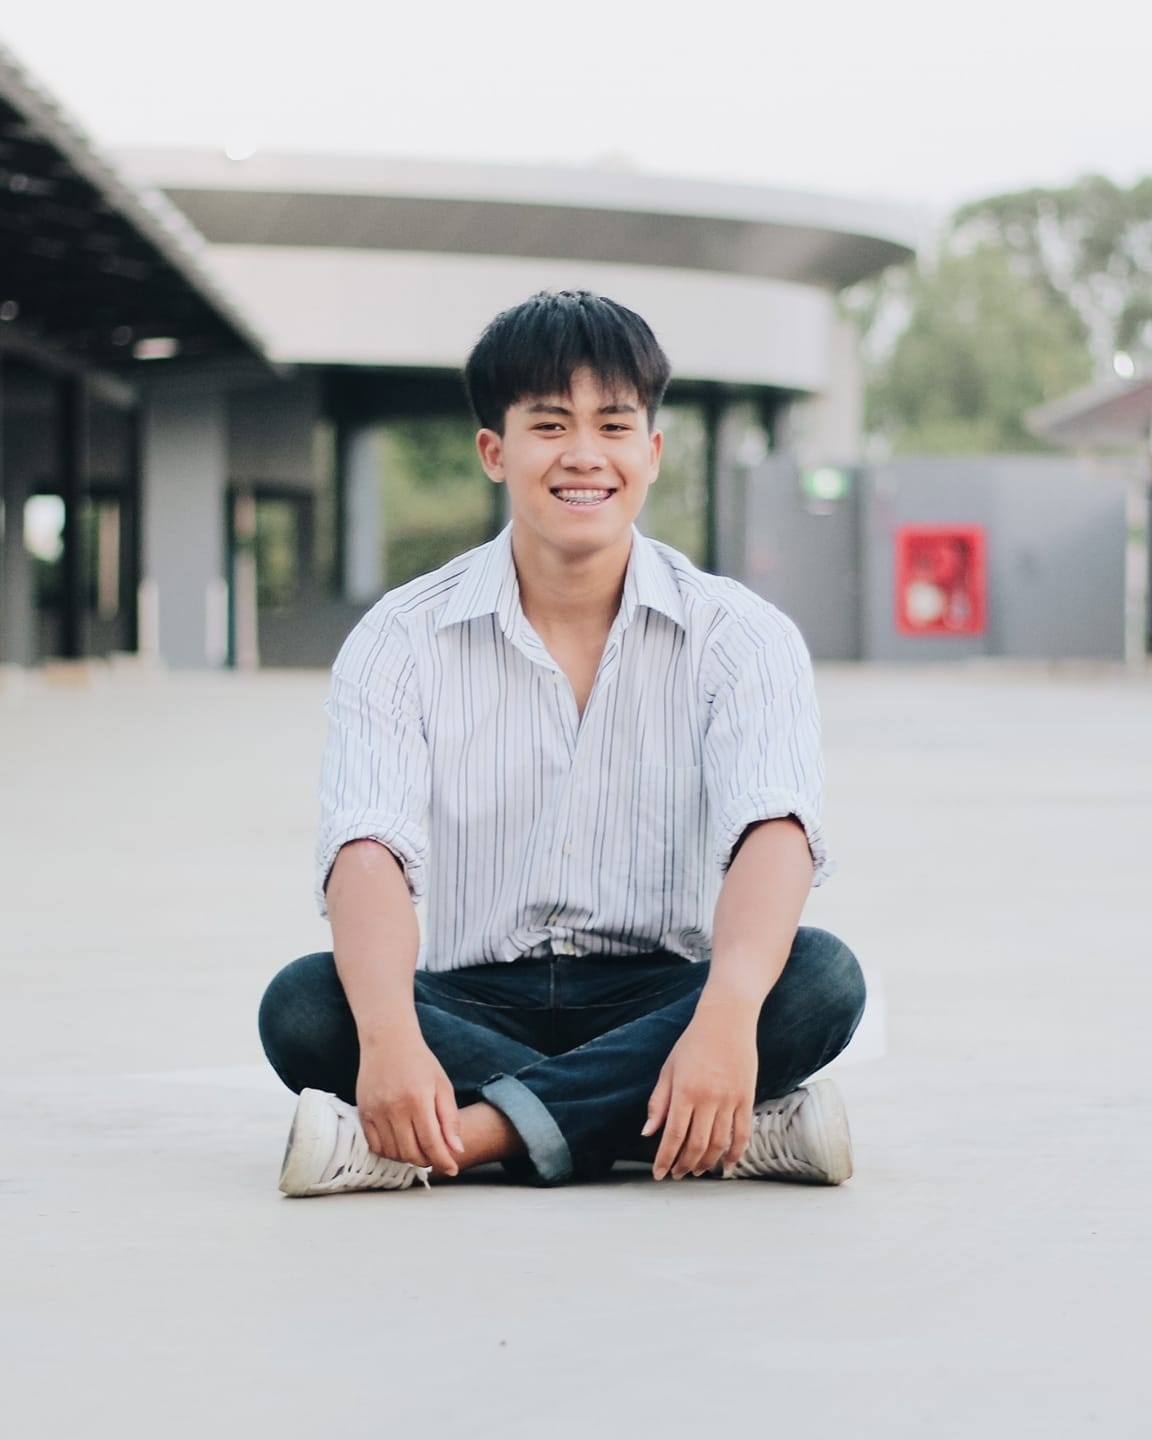
\includegraphics[width=1.5in]{./image/profile_kao.jpg}
\end{center}
นายอภิเทพ ปิยพิพัฒนมงคล นักศึกษาชั้นปี ที่ 4 คณะวิศวกรรมศาสตร์ สาขาวิศวกรรมคอมพิวเตอร์ มหาวิทยาลัยเชียงใหม่
\end{biosketch}
\fi % \ifproject
\end{document}
